%%%%%%%%%%%%%%%%%%%%%%%%%%%%%%%%%%%%%%%%%%%%%%%%%%%%%%%%%%%%%%%
%% OXFORD THESIS TEMPLATE

% Use this template to produce a standard thesis that meets the Oxford University requirements for DPhil submission
%
% Originally by Keith A. Gillow (gillow@maths.ox.ac.uk), 1997
% Modified by Sam Evans (sam@samuelevansresearch.org), 2007
% Modified by John McManigle (mcmanigle@gmail.com), 2015

% I've (John) tried to comment this file extensively, so read through it to see how to use the various options.  Remember
% that in LaTeX, any line starting with a % is NOT executed.  Several places below, you have a choice of which line to use
% out of multiple options (eg draft vs final, for PDF vs for binding, etc.)  When you pick one, add a % to the beginning of
% the lines you don't want.


%%%%% CHOOSE PAGE LAYOUT
% The most common choices should be below.  You can also do other things, like replacing "a4paper" with "letterpaper", etc.

% This one will format for two-sided binding (ie left and right pages have mirror margins; blank pages inserted where needed):
% FINAL Switch to binding format
% FINAL Consider if I want to remove the hidelinks option
%\documentclass[hidelinks,a4paper,twoside]{ociamthesis}
% This one will format for one-sided binding (ie left margin > right margin; no extra blank pages):
%\documentclass[hidelinks, a4paper]{ociamthesis}
% This one will format for PDF output (ie equal margins, no extra blank pages):
\documentclass[hidelinks, a4paper,nobind]{ociamthesis} 



%%%%% SELECT YOUR DRAFT OPTIONS
% Three options going on here; use in any combination.  But remember to turn the first two off before
% generating a PDF to send to the printer!

% This adds a "DRAFT" footer to every normal page.  (The first page of each chapter is not a "normal" page.)
% FINAL remove Draft Remark
\fancyfoot[C]{\emph{DRAFT Printed on \today}}  

% This highlights (in blue) corrections marked with (for words) \mccorrect{blah} or (for whole
% paragraphs) \begin{mccorrection} . . . \end{mccorrection}.  This can be useful for sending a PDF of
% your corrected thesis to your examiners for review.  Turn it off, and the blue disappears.
%\correctionstrue


%%%%% BIBLIOGRAPHY SETUP
% Note that your bibliography will require some tweaking depending on your department, preferred format, etc.
% The options included below are just very basic "sciencey" and "humanitiesey" options to get started.
% If you've not used LaTeX before, I recommend reading a little about biblatex/biber and getting started with it.
% If you're already a LaTeX pro and are used to natbib or something, modify as necessary.
% Either way, you'll have to choose and configure an appropriate bibliography format...

% The science-type option: numerical in-text citation with references in order of appearance.
\usepackage[style=numeric-comp, sorting=none, backend=biber, doi=false, isbn=false]{biblatex}
\newcommand*{\bibtitle}{References}

% The humanities-type option: author-year in-text citation with an alphabetical works cited.
%\usepackage[style=authoryear, sorting=nyt, backend=biber, maxcitenames=2, useprefix, doi=false, isbn=false]{biblatex}
%\newcommand*{\bibtitle}{Works Cited}

% This makes the bibliography left-aligned (not 'justified') and slightly smaller font.
\renewcommand*{\bibfont}{\raggedright\small}

% Change this to the name of your .bib file (usually exported from a citation manager like Zotero or EndNote).
\addbibresource{references.bib}


% Uncomment this if you want equation numbers per section (2.3.12), instead of per chapter (2.18):
%\numberwithin{equation}{subsection}



%%%%% THESIS / TITLE PAGE INFORMATION
% Everybody needs to complete the following:
\title{Deep Learning for \\Counterfactual Inference}
\author{Michael Weisz}
\college{Green Templeton College}

% Master's candidates who require the alternate title page (with candidate number and word count)
% must also un-comment and complete the following three lines:
% META Check what the title page should look like (candidate number?)
%\masterssubmissiontrue
%\candidateno{933516}
%\wordcount{28,815}

% Uncomment the following line if your degree also includes exams (eg most masters):
\renewcommand{\submittedtext}{A dissertation submitted in partial completion of the degree}
% Your full degree name.  (But remember that DPhils aren't "in" anything.  They're just DPhils.)
\degree{MSc in Computer Science}
% Term and year of submission, or date if your board requires (eg most masters)
%\degreedate{August 29, 2017}
\degreedate{Trinity 2017}


%%%%% YOUR OWN PERSONAL MACROS
% This is a good place to dump your own LaTeX macros as they come up.

% To make text superscripts shortcuts
	\renewcommand{\th}{\textsuperscript{th}} % ex: I won 4\th place
	\newcommand{\nd}{\textsuperscript{nd}}
	\renewcommand{\st}{\textsuperscript{st}}
	\newcommand{\rd}{\textsuperscript{rd}}


% Make Headings align left
\makeatletter
\renewcommand{\@makechapterhead}[1]{\chapterheadstartvskip%
	{\size@chapter{\sectfont
			{\chapnumfont
				\ifnum \c@secnumdepth >\m@ne%
				\if@mainmatter\noindent\thechapter%
				\fi\fi
				\par\nobreak}%
			{\interlinepenalty\@M\noindent #1\par}}
		\nobreak\chapterheadendvskip}}
\makeatother


%%%%%%%% My packages
%\usepackage[nolist,nohyperlinks]{acronym}
\usepackage{nameref}
\usepackage{float}
\usepackage{wrapfig}
\usepackage{amsmath}
\usepackage{booktabs}
\usepackage{algorithm}
\usepackage[noend]{algpseudocode}
\usepackage{subcaption}
\usepackage[parfill]{parskip}

%%%%%%%


%%%%%%%% Acronyms
%\acrodef{DCN}[DCN]{\emph{DCN}}

%%%%%%%%

%%%%% THE ACTUAL DOCUMENT STARTS HERE
\begin{document}



%%%%% CHOOSE YOUR LINE SPACING HERE
% This is the official option.  Use it for your submission copy and library copy:
%\setlength{\textbaselineskip}{22pt plus2pt}
% This is closer spacing (about 1.5-spaced) that you might prefer for your personal copies:
\setlength{\textbaselineskip}{18pt plus2pt minus1pt}

% You can set the spacing here for the roman-numbered pages (acknowledgements, table of contents, etc.)
\setlength{\frontmatterbaselineskip}{17pt plus1pt minus1pt}

% Leave this line alone; it gets things started for the real document.
\setlength{\baselineskip}{\textbaselineskip}


%%%%% CHOOSE YOUR SECTION NUMBERING DEPTH HERE
% You have two choices.  First, how far down are sections numbered?  (Below that, they're named but
% don't get numbers.)  Second, what level of section appears in the table of contents?  These don't have
% to match: you can have numbered sections that don't show up in the ToC, or unnumbered sections that
% do.  Throughout, 0 = chapter; 1 = section; 2 = subsection; 3 = subsubsection, 4 = paragraph...

% The level that gets a number:
\setcounter{secnumdepth}{2}
% The level that shows up in the ToC:
\setcounter{tocdepth}{2}


%%%%% ABSTRACT SEPARATE
% This is used to create the separate, one-page abstract that you are required to hand into the Exam
% Schools.  You can comment it out to generate a PDF for printing or whatnot.
% META Check if I need the separate abstract page (uncomment below)
%\begin{abstractseparate}
%	Your abstract text goes here.  Check your departmental regulations, but generally this should be less than 300 words.  See the beginning of Chapter~\ref{ch:2-litreview} for more.

Lorem ipsum dolor sit amet, consectetur adipiscing elit. Pellentesque sit amet nibh volutpat, scelerisque nibh a, vehicula neque. Integer placerat nulla massa, et vestibulum velit dignissim id. Ut eget nisi elementum, consectetur nibh in, condimentum velit. Quisque sodales dui ut tempus mattis. Duis malesuada arcu at ligula egestas egestas. Phasellus interdum odio at sapien fringilla scelerisque. Mauris sagittis eleifend sapien, sit amet laoreet felis mollis quis. Pellentesque dui ante, finibus eget blandit sit amet, tincidunt eu neque. Vivamus rutrum dapibus ligula, ut imperdiet lectus tincidunt ac. Pellentesque ac lorem sed diam egestas lobortis.

Suspendisse leo purus, efficitur mattis urna a, maximus molestie nisl. Aenean porta semper tortor a vestibulum. Suspendisse viverra facilisis lorem, non pretium erat lacinia a. Vestibulum tempus, quam vitae placerat porta, magna risus euismod purus, in viverra lorem dui at metus. Sed ac sollicitudin nunc. In maximus ipsum nunc, placerat maximus tortor gravida varius. Suspendisse pretium, lorem at porttitor rhoncus, nulla urna condimentum tortor, sed suscipit nisi metus ac risus.

Aenean sit amet enim quis lorem tristique commodo vitae ut lorem. Duis vel tincidunt lacus. Sed massa velit, lacinia sed posuere vitae, malesuada vel ante. Praesent a rhoncus leo. Etiam sed rutrum enim. Pellentesque lobortis elementum augue, at suscipit justo malesuada at. Lorem ipsum dolor sit amet, consectetur adipiscing elit. Praesent rhoncus convallis ex. Etiam commodo nunc ex, non consequat diam consectetur ut. Pellentesque vitae est nec enim interdum dapibus. Donec dapibus purus ipsum, eget tincidunt ex gravida eget. Donec luctus nisi eu fringilla mollis. Donec eget lobortis diam.

Suspendisse finibus placerat dolor. Etiam ornare elementum ex ut vehicula. Donec accumsan mattis erat. Quisque cursus fringilla diam, eget placerat neque bibendum eu. Ut faucibus dui vitae dolor porta, at elementum ipsum semper. Sed ultrices dui non arcu pellentesque placerat. Etiam posuere malesuada turpis, nec malesuada tellus malesuada. % Create an abstract.tex file in the 'text' folder for your abstract.
%\end{abstractseparate}


% Pages are roman numbered from here, though page numbers are invisible until ToC.  This is in
% keeping with most typesetting conventions.
\begin{romanpages}

% Title page is created here
\maketitle

%%%%% DEDICATION -- If you'd like one, un-comment the following.
% NICE TO HAVE: Think about having a dedication
%\begin{dedication}
%This thesis is dedicated to\\
%someone\\
%for some special reason\\
%\end{dedication}

%%%%% ACKNOWLEDGEMENTS -- Nothing to do here except comment out if you don't want it.
\begin{acknowledgements}
 	%Here be dragons...


This dissertation concludes the findings of my master project \emph{Deep Learning for Counterfactual Inference} at the University of Oxford. I am taking this opportunity to express my sincere gratitude to all the people who helped me along the way and ultimately made this possible.

Firstly, I would like to thank my supervisor Prof. Dr. Mihaela van der Schaar for her guidance and for showing me an exciting problem to work on. In addition, I was fortunate to be working with her PhD student Ahmed Alaa who provided valuable feedback and fresh ideas whenever I was struggling. 

Furthermore, I would like to acknowledge my secondary supervisor Prof. Dr. Edith Elkind, my departmental supervisor Dr. Milos Nikolic, and  my academic advisor Dr. Garrett Morris of Green Templeton College for their guidance throughout this year. 

A master's program can be challenging on many levels. Therefore, I am grateful for the community and encouragements I received from the inhabitants of 39 St. Margaret's Road and my friends from the department and Green Templeton College who made this year such an unforgettable experience. 

Most of all, I would like to thank my father Jenö, my mother Ingrid, my sister Elisabeth, and my girlfriend Albana for their unfailing support  --- day-and-night even in the most stressful situations. 

I would not have been able to do it without you. 

\begin{flushright}
Michael 
\end{flushright}

%This is where you thank your advisor, colleagues, and family and friends.

% Supervisor: Mihaela + Ahmed
% My friends 
% Rosi und Papa
% Lisi
% Albana
	

\end{acknowledgements}

%%%%% ABSTRACT -- Nothing to do here except comment out if you don't want it.
\begin{abstract}
	Your abstract text goes here.  Check your departmental regulations, but generally this should be less than 300 words.  See the beginning of Chapter~\ref{ch:2-litreview} for more.

Lorem ipsum dolor sit amet, consectetur adipiscing elit. Pellentesque sit amet nibh volutpat, scelerisque nibh a, vehicula neque. Integer placerat nulla massa, et vestibulum velit dignissim id. Ut eget nisi elementum, consectetur nibh in, condimentum velit. Quisque sodales dui ut tempus mattis. Duis malesuada arcu at ligula egestas egestas. Phasellus interdum odio at sapien fringilla scelerisque. Mauris sagittis eleifend sapien, sit amet laoreet felis mollis quis. Pellentesque dui ante, finibus eget blandit sit amet, tincidunt eu neque. Vivamus rutrum dapibus ligula, ut imperdiet lectus tincidunt ac. Pellentesque ac lorem sed diam egestas lobortis.

Suspendisse leo purus, efficitur mattis urna a, maximus molestie nisl. Aenean porta semper tortor a vestibulum. Suspendisse viverra facilisis lorem, non pretium erat lacinia a. Vestibulum tempus, quam vitae placerat porta, magna risus euismod purus, in viverra lorem dui at metus. Sed ac sollicitudin nunc. In maximus ipsum nunc, placerat maximus tortor gravida varius. Suspendisse pretium, lorem at porttitor rhoncus, nulla urna condimentum tortor, sed suscipit nisi metus ac risus.

Aenean sit amet enim quis lorem tristique commodo vitae ut lorem. Duis vel tincidunt lacus. Sed massa velit, lacinia sed posuere vitae, malesuada vel ante. Praesent a rhoncus leo. Etiam sed rutrum enim. Pellentesque lobortis elementum augue, at suscipit justo malesuada at. Lorem ipsum dolor sit amet, consectetur adipiscing elit. Praesent rhoncus convallis ex. Etiam commodo nunc ex, non consequat diam consectetur ut. Pellentesque vitae est nec enim interdum dapibus. Donec dapibus purus ipsum, eget tincidunt ex gravida eget. Donec luctus nisi eu fringilla mollis. Donec eget lobortis diam.

Suspendisse finibus placerat dolor. Etiam ornare elementum ex ut vehicula. Donec accumsan mattis erat. Quisque cursus fringilla diam, eget placerat neque bibendum eu. Ut faucibus dui vitae dolor porta, at elementum ipsum semper. Sed ultrices dui non arcu pellentesque placerat. Etiam posuere malesuada turpis, nec malesuada tellus malesuada.
\end{abstract}

%%%%% MINI TABLES
% This lays the groundwork for per-chapter, mini tables of contents.  Comment the following line
% (and remove \minitoc from the chapter files) if you don't want this.  Un-comment either of the
% next two lines if you want a per-chapter list of figures or tables.
% NICE TO HAVE: Do I want a mini toc in each chapter? 
%\dominitoc % include a mini table of contents
%\dominilof  % include a mini list of figures
%\dominilot  % include a mini list of tables

% This aligns the bottom of the text of each page.  It generally makes things look better.
\flushbottom

% This is where the whole-document ToC appears:
\tableofcontents

%\listoffigures
%	\mtcaddchapter
% \mtcaddchapter is needed when adding a non-chapter (but chapter-like) entity to avoid confusing minitoc

% Uncomment to generate a list of tables:
%\listoftables
%	\mtcaddchapter

%%%%% LIST OF ABBREVIATIONS
% This example includes a list of abbreviations.  Look at text/abbreviations.tex to see how that file is
% formatted.  The template can handle any kind of list though, so this might be a good place for a
% glossary, etc.
%% First parameter can be changed eg to "Glossary" or something.
% Second parameter is the max length of bold terms.
\begin{mclistof}{List of Abbreviations}{3.2cm}

\item[1-D, 2-D] One- or two-dimensional, referring in this thesis to spatial dimensions in an image.

\item[Otter] One of the finest of water mammals.

\item[Hedgehog] Quite a nice prickly friend.

\end{mclistof} 


% The Roman pages, like the Roman Empire, must come to its inevitable close.
\end{romanpages}


%%%%% CHAPTERS
% Add or remove any chapters you'd like here, by file name (excluding '.tex'):
\flushbottom
\part{Introduction}
%\begin{savequote}[8cm]
%\textlatin{Jedem Anfang wohnt ein Zauber innne.}
%
%In the core of every beginning lives magic.
%  \qauthor{--- Hermann Hesse's \textit{Stufen}}
%\end{savequote}

\chapter{\label{ch:1-intro}Introduction} 

%\minitoc

\section{Motivation}


\section{Scope and Contribution}

\section{Thesis Structure}


%\begin{savequote}[8cm]
%\textlatin{Jedem Anfang wohnt ein Zauber innne.}
%
%In the core of every beginning lives magic.
%  \qauthor{--- Hermann Hesse's \textit{Stufen}}
%\end{savequote}

\chapter{\label{ch:2-background}Theoretical Background} 

%\minitoc
\section{Introduction}  
This chapter introduces the relevant background for our project and its related work. 
We start by providing an introduction to the field of machine learning, its terminology, and core concepts such as model definitions, objective functions, training methods, and regularisation. The second part of the chapter deals with the specifics of \emph{deep learning} which is a  subfield of machine learning that utilises a certain class of models called \emph{deep neural networks}. We outline different types of neural networks and their respective topologies before discussing concepts like multi-task learning and dropout. The final part of the chapter is dedicated to the problem of counterfactual inference. We motivate the importance of the task and its application areas, and provide a formalisation. Furthermore, we outline the challenges of the problem and different existing approaches that have been applied to it so far. 

%We conclude by relating counterfactual inference to deep learning and describing its open research questions which is the very foundation of this thesis. 

\section{Machine Learning}

\subsection{Motivation}
When conceptualising computer programs, we often think of them as series of discrete, unambiguous, sequential instructions that are executed in a deterministic way and have to be explicitly programmed by a human programmer. 

Many problems --- in particular those for which a well-defined algorithm or effective step-by-step solution strategy exists --- can be successfully expressed and ultimately solved this way. 

Nonetheless, there are domains where this algorithmic approach seems infeasible. A typical example is autonomous driving for which there are almost infinitely many possible situations to consider making it impossible to encode the desired behaviour of an autonomous vehicle as a finite sequence of instructions. 

One potential way to approach these kinds of problems is by using a concept called \emph{machine learning} which is a subfield of computer science that deals with the question of how to teach computer programs to learn to perform a task without being explicitly programmed how to do it. 
% PLAG? Check if this it too close to the quote at wikipedia 

More formally, a common definition of machine learning suggests that an algorithm "is said to learn from experience E with respect to some class of tasks T and performance measure P if its performance at tasks in T, as measured by P, improves with experience E." \cite{ml-definition}
% PLAG?

Transferred to our example of autonomous driving, we could define the task $T$ in terms of "moving the car from an origin A to a destination B" while our performance measure $P$ might include aspects such as the travel time the number of damaged objects or harmed humans. The experience $E$ would represent so called \emph{training data} that is acquired by previously covered distances (either autonomously or by recording the actions of a human driver). 

% TODO Show diagram (model, algorithm, learning, data)

\subsection{Types of Learning}
Machine Learning is typically categorised into three main categories which are briefly outlined in the following. 

\subsubsection{Supervised Learning} 
In a supervised learning setting, the task is to infer a function from a number of samples from a training dataset that is said to be \emph{labelled}. In other words, for each sample in the training data, we have access to the actual function value we want to predict while training the model. 

For instance, we might be interested in predicting housing prices where we are given a dataset consisting of information regarding different properties (e.g. the number of rooms and the area in $m^2$), commonly referred  to as \emph{features} or \emph{covariates}, and the actual price for which the house has been sold, called \emph{outcome}, \emph{target}, or \emph{label}. 

Once the \emph{model has been trained} --- i.e. we have found the parameters of an appropriate function that best describes the historic dataset --- we can use the same model to predict the housing prices for unseen data points. 

Such a task of predicting a continuous variable is often referred to as a \emph{regression problem} whereas the prediction of a discrete output is called a \emph{classification problem}. 

\subsubsection{Unsupervised Learning} 
In contrast to supervised learning, the training set of an unsupervised learning problem does not contain the target labels. Typical tasks in this setting include inferring structural patterns from the data and \emph{clustering }it accordingly. 

It is important to note that for supervised learning, there is normally no concept of an underlying \emph{ground-truth} that we are trying to predict. In other words, the performance (or quality) of the outcome typically cannot be measured or defined in absolute terms but depends on the domain-specific use-case of the clustering. 

Another important task in unsupervised learning is \emph{dimensionality reduction} for which a high-dimensional dataset is reduced to a target lower dimension while simultaneously trying to minimise the information loss. 

\subsubsection{Reinforcement Learning}
In reinforcement learning, a software agent has to learn a sequence of appropriate actions in a dynamic environment in which the consequences of an action might not be immediately accessible but accumulate to a long-term reward that ought to be maximised. \cite{reinforcement-learning}

A most prominent example was mentioned earlier with the task of autonomous driving in which a vehicle is governed by a piece of software that has to find an adequate series of actions (i.e. steering and regulating speed) in order to reach a target destination in a complex and dynamically changing environment. 

\subsection{Machine Learning Models}
% GRAPH Re-create graph!
\begin{figure}[h]
	\caption{Schematic Approach of Machine Learning. A selected model $M$ is trained on a dataset $D$ using a learning algorithm $A$.} \label{fig:machine-learning-approach}
	\centering
	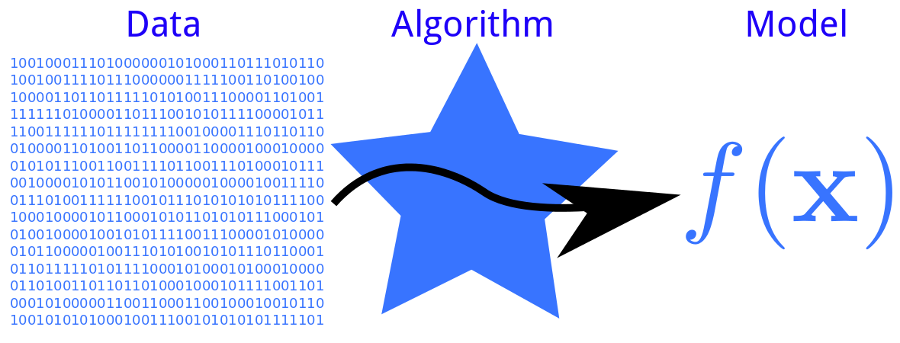
\includegraphics[width=0.5\textwidth]{figures/chapter-2/machine-learning-approach.png}
\end{figure} 

Machine learning is based on the concept of selecting an appropriate model and fitting it to a given (training) data set using a training algorithm illustrated in figure \ref{fig:machine-learning-approach}. 

For instance, we might want to use a \emph{linear model} $f$ for our task of predicting housing prices
\begin{equation}
f_{\mathbf{w}, b}(\mathbf{x}) = \mathbf{w}\cdot \mathbf{x} + b,
\end{equation}
where $\mathbf{x}$ corresponds to the input vector containing the features of the house, and $\mathbf{w}, b$ represent the parameters of our linear model commonly referred to as \emph{weights} and \emph{bias}. We can then make use \emph{linear regression} to fit our linear model to our labelled dataset of existing houses and their prices. 

The selection of an appropriate model is of great importance and determines factors such as the trade-off between the expressiveness or \emph{variance} of the model (i.e. its ability to capture complex relationships) and its potential to generalise to unseen data points. Additionally,  computational considerations such as time and space complexity of the model and its training process have to be taken into account. 

Consequently, the selection of an appropriate model typically depends on the task, the training datasets, and its characteristics. Typical alternatives to the linear model include \emph{support vector machines}, \emph{decision trees}, and \emph{neural networks}. 
% TODO What are other typical models. How do they compare against each other? 
% Should I sketch them out here? 

This dissertation focuses on using \emph{deep learning} for the problem of counterfactual inference. Therefore, a dedicated part of this chapter deals exclusively with deep neural networks and describes their characteristics in more detail. 


\subsection{Variance, Bias, and Regularisation} \label{sec:regularisation}
% GRAPH Re-create graph!
\begin{figure}[]
	\centering
	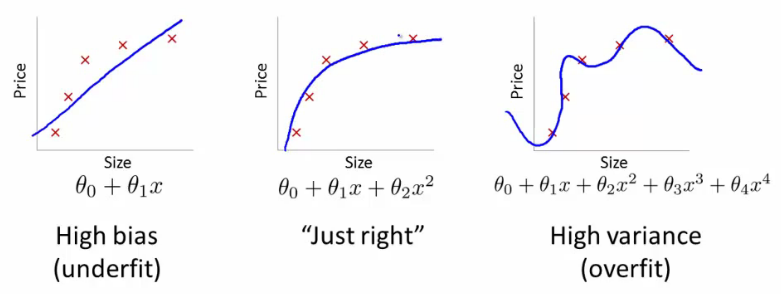
\includegraphics[width=0.8\textwidth]{figures/chapter-2/overfitting-underfitting.png}
	\caption{Visualisation of Bias variance Tradeoff. The model on the left is ... whereas the middle one ... and the right one is ...}	\label{fig:overfitting-underfitting}
\end{figure}
When training our model we have to find the right balance between fitting it most accurately to the training data while making sure that it still generalises well to unseen data points. This consideration is commonly referred to as \emph{trade-off between bias and variance},  illustrated in figure \ref{fig:overfitting-underfitting}. 

The model on the left tries to fit a straight line to a dataset which expresses polynomial properties resulting in a poor approximation often referred to as \emph{underfitting}. We might say the model has a high \emph{bias} and is therefore too simple to accurately describe the relationship in the data. 

In contrast, the model on the right uses high-order polynomial features and is able to perfectly fit the data resulting in a training error of zero. This, however, is typically not desired as we would merely "memorise" the training data and perform poorly on any unseen future data points. In other words, we are \emph{overfitting} the training dataset because of a \emph{high variance}.  

Consequently, the objective is to train a model that neither overfits nor underfits the training data and generalises well to unseen datapoints ( illustrated by the model in the middle). 

The most common approach to achieve this is by selecting a model which is likely to have a sufficient variance to capture the complexity of the data (thus avoiding underfitting) and then making use of a concept called \emph{regularisation} to avoid overfitting. 

Regularisation can be achieved by introducing a \emph{regularisation term} in the objective function that imposes a penalty for learning models that are too complex. Consider the terms 
\begin{align} 
R_{l1}(\mathbf{w}) = \sum_{i=1}^{d}  \lvert \mathbf{w}_i \lvert  && \text{and} &&R_{l2}(\mathbf{w}) = \sum_{i=1}^{d}  \mathbf{w}_i^2,
\end{align} 

where $d$ refers to the dimension of the weights parameter $\mathbf{w}$, that both penalise the sum of the weights (in terms of the absolute value or as a quadratic function, respectively). This way, we ensure that the model learns the parameters in a way that only attaches high weights to highly predictive features since their gain has to outweigh the penalty imposed by the regularisation term. 
 
We will cover the concept of regularisation in more detail in section \ref{sec:dropout} for neural networks as they represent the class of models that this thesis is focus on. 


%When using a complex model with a high variance, we might naively fit our model to the training data perfectly, resulting in a training error of zero. This, however, would merely "memorise" the training data and might perform poorly on unseen future data points. This phenomenon where we overfit the training data is often referred to as \emph{high variance}. 
%In contrast, if the model is too simple, we night not be able to accurately capture the relationship in our data leading to equally poor results. In this case, we are under-fitting the data and our model has a so called \emph{high bias}.
%
%


% TODO Should I include learning curves as well? 
%% TODO! Re-create graph!
%\begin{figure}[]
%	\label{fig:machine-learning-approach}
%	\caption{Visualisation of Learning Curves. The left model is ... whereas the right model is ...}
%	\centering
%	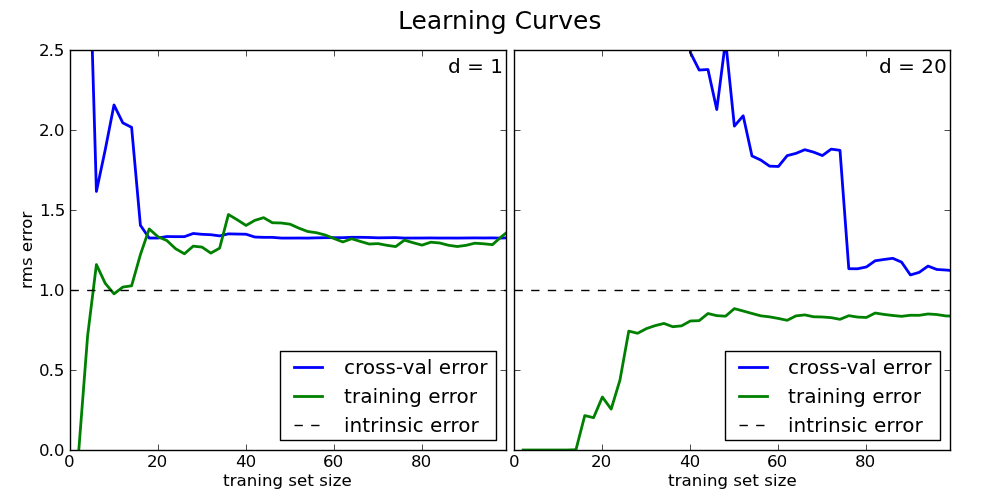
\includegraphics[width=0.8\textwidth]{figures/chapter-2/learning-curves.png}
%\end{figure}




\section{Deep Learning}
\subsection{Introduction}
Deep learning refers to a field of machine learning that is based on the use of so called \emph{deep neural networks}. 

The approach is loosely inspired by how the human brain works,  modelling biological neurons and their interconnections in terms of artificial neurons that express similar properties.


\paragraph{Biological Foundations}
The details about our understanding of the mechanics and biochemical processes of the human brain are well beyond the scope of this thesis. On a conceptual level, however, each neuron receives inputs signals on its dendrites which are connected to the axons of neighbouring neurons. The input signals are accumulated and processed within the cell body causing the cell to output a signal on its own axon (in turn representing a potential input for other cells). By means of these interconnections, the neurons form a highly complex structure that can be conceptualised in terms of a biological neural network. It is estimated that the human brain contains about 100 billion neurons  allowing it to process complex signals and reason about abstract concepts \cite{number-of-neurons}. 
% TODO What about learning? 

In a bionic fashion, an \emph{artificial neural network} (henceforth called \emph{neural network}), adopts this architecture in a simplified way by defining a network of \emph{artificial neurons} (discussed in details in section \ref{sec:mlp}) that are connected according to a certain topology. The analogy between the human and the artificial neurons is illustrated in figure \ref{fig:artificial-neuron}: The artificial neuron receives input signals, processes the signals according to an internal activation function, and outputs a computed signal on its own. 

Analogous to its biological counterpart the a neural network is able to capture complex non-linear relationships to approximate arbitrarily complex functions. 



% GRAPH Recreate graph
\begin{figure}[h]
	\caption{A biological neuron vs. an artificial neuron}\label{fig:biological-vs-artificial-neuron}
	\centering
	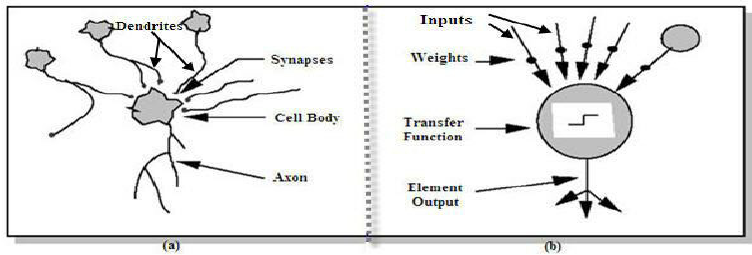
\includegraphics[width=0.8\textwidth]{figures/chapter-2/biological-vs-artificial-neurons.png}
\end{figure}


\paragraph{History of Neural Networks}The theoretical foundations of neural networks date back to the 1940s \cite{nn-history}, before becoming popular in the 1970s after the \emph{backpropagation algorithm} (see section \ref{sec:training}) had been successfully applied to neural networks  \cite{backprop1}. Following an initial enthusiasm, however, neural networks fell out of favour in the following decades due to the realisation that the models typically expressed a degree of computational complexity that could not be accommodated by the existing hardware.

This changed again in the early 2010s when a neural networks significantly outperformed existing methods in a variety of fields such as computer vision \cite{imagenet} and natural language processing \cite{nlp}. % CITE imagenet

Ever since, deep neural networks have been responsible for some of the most recent successes in machine learning, including self-driving cars and defeating human champions in the game of Go \cite{alphago}.
The renaissance of neural networks and its recent successes have typically been attributed to two key factors: Firstly, the advancements in computational capabilities on modern GPUs and other highly-optimised processing units such as \emph{FPGAs} and \emph{ASICS}.
Secondly, the widespread availability of large datasets that can be used for training the models such as web-scale text corpora for natural language processing or large databases of images that can be used in computer vision. 

\paragraph{Status Quo} Today, deep neural networks represent the state-of-the-art for many problems. They are widely considered one of the most promising areas of machine learning and artificial intelligence in general and have received a high level of attention in society, media, and politics. Nevertheless, the usage of deep neural networks poses a multitude of computational, architectural, and domain-specific questions that are the subject of ongoing research. 

\subsection{The Multilayer Perceptron} \label{sec:mlp}
In order to understand how neural networks work, we first investigate one of its most basic forms: the \emph{multilayer perceptron} or MLP. 

% GRAPH Redo graph
\begin{figure}[H]
% GRAPH-LABEL Add proper description
\centering
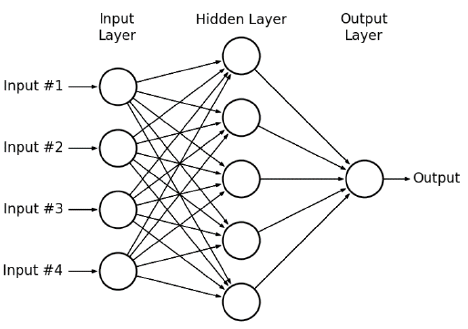
\includegraphics[width=0.7\textwidth]{figures/chapter-2/multilayer-perceptron.png}
\caption{Prototypical multilayer perceptron with a single hidden layer.}\label{fig:multilayer-perceptron}
\end{figure}
Figure \ref{fig:multilayer-perceptron} depicts the schematics of a MLP. As the name suggests, it consists of multiple layers each containing a fixed number of artificial neurons (henceforth called neurons) that are interconnected exclusively by neurons of neighbouring layers. The first, so called \emph{input layer}, is followed by one or more \emph{hidden layers} leading to a final so called \emph{output layer}. 

\begin{figure}[h]
	\centering
	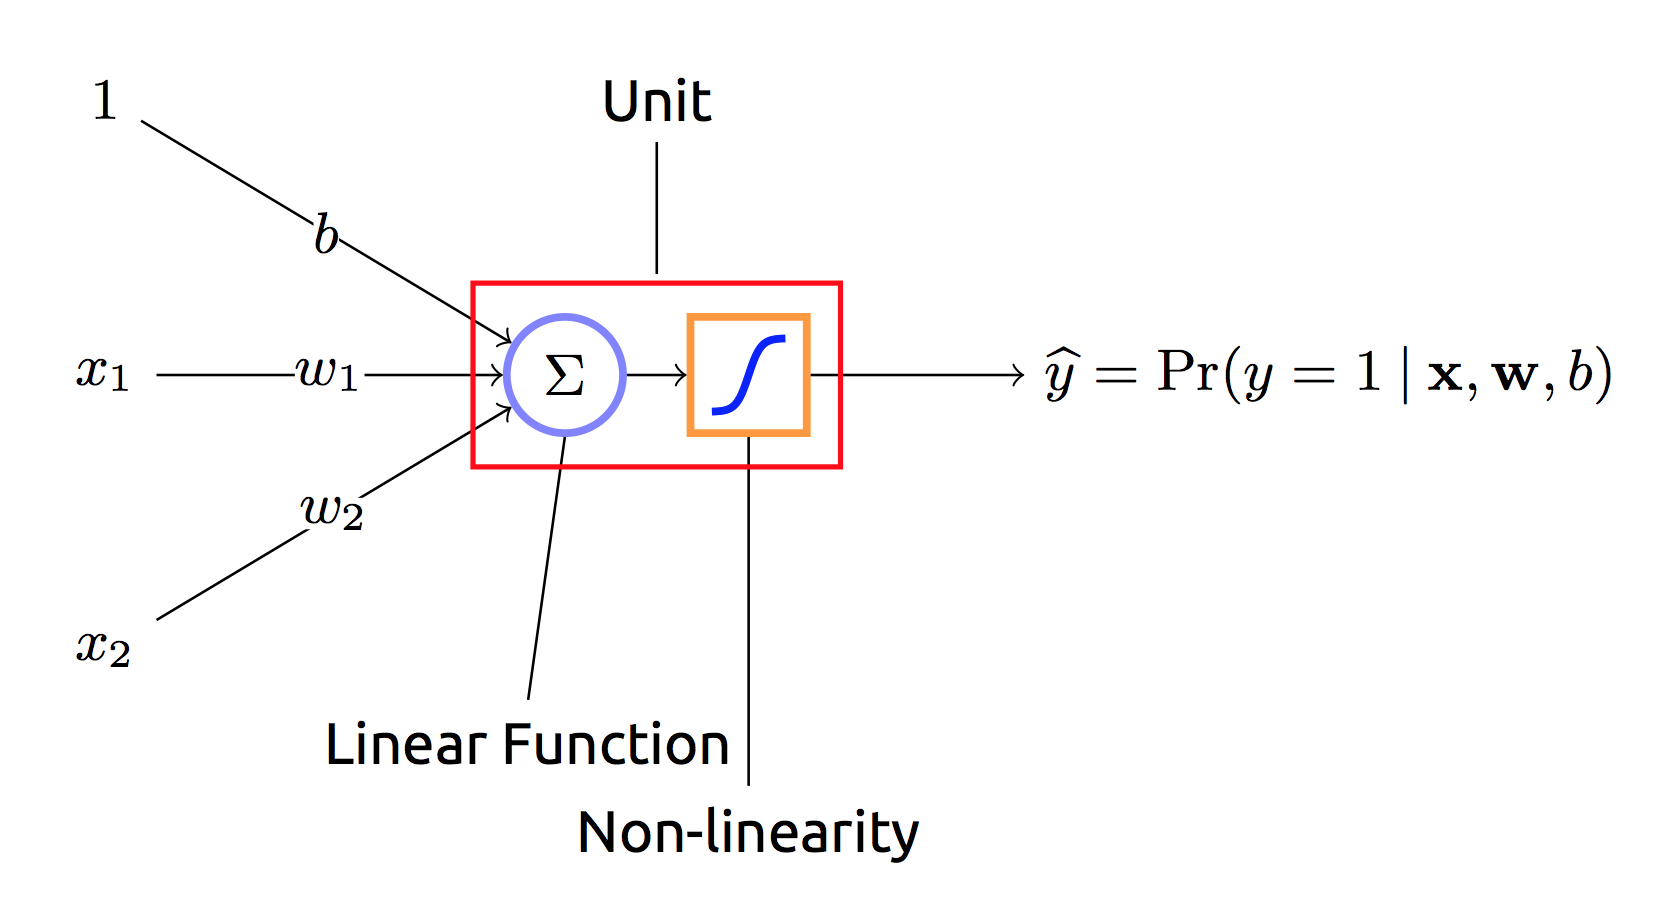
\includegraphics[width=0.6\textwidth]{figures/chapter-2/artificial-neuron.png}
	\caption{Basic building block: Artificial Neuron used for classification.}\label{fig:artificial-neuron}   
\end{figure}

In a MLP, the basic building block is the artificial neuron or \emph{unit} which is illustrated in figure \ref{fig:artificial-neuron}. 

Its output $y$ is computed as 
\begin{equation}
	% MATHS Check, looks weird with b in front
	y = \phi(b + \sum_{i=1}^{n} w_i x_i)
\end{equation}
where $x_1, \ldots, x_n \in \mathbb{R}$ corresponds to the inputs of the neuron, $w_1, \dots, w_n\in \mathbb{R}$ to the weights and $b \in \mathbb{R}$ to a bias ($w$ and  $b$ are the parameters of the model that ought to be learnt) and $\phi: \mathbb{R} \rightarrow \mathbb{R}$ to a non-linear function referred to as \emph{activation function}. Typical choices for $\phi$ include 
\begin{align*} 
\phi(x) = \sigma(x) = \frac{1}{1 + e^{-x}} && \text{or} && \phi(x) = tanh(x) = \frac{1  - e^{-2x}}{1  + e^{-2x}}
\end{align*} 
where $\sigma(x)$ refers to the \emph{sigmoid function}, $tanh(x)$ to the \emph{hyperbolic tangent}, and $ReLU$ to \emph{rectified linear unit}. While each of these activation functions has different properties as illustrated in figure \ref{fig:activation-functions}, a typical characteristic is that they map the input value to the closed interval $[0, 1]$. 

% GRAPH Add plots for sigmoid, tnah, and relu
\begin{figure}[h]
	\caption{Typical Activation functions}\label{fig:activation-functions}   
	\centering
	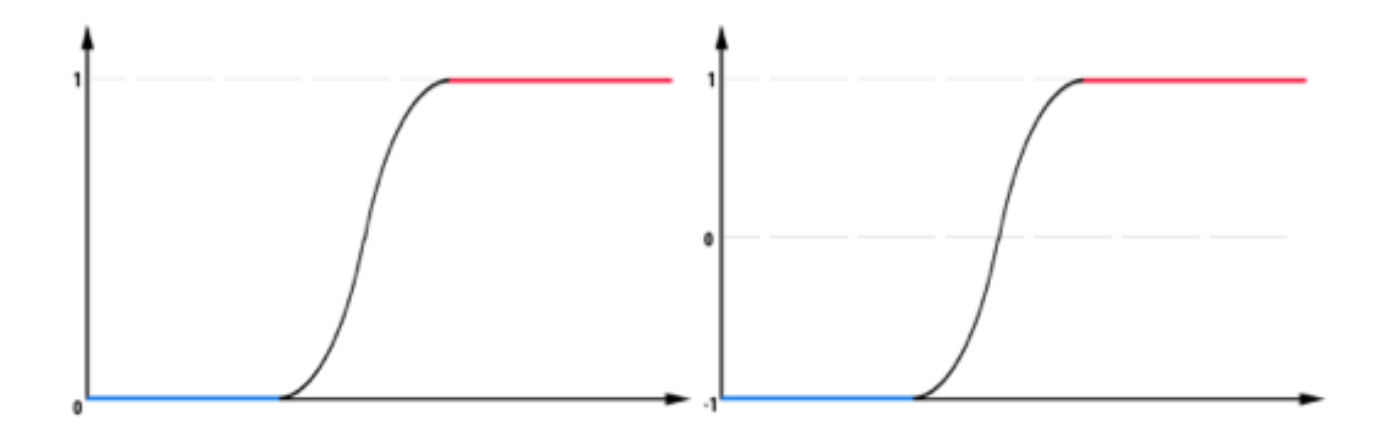
\includegraphics[width=0.6\textwidth]{figures/chapter-2/activation-functions.png}
\end{figure}


% TODO What else do I need to write about MLPs?  Equations for the outcome? 
%Given this definition of a single unit, the final value $y$ of the outcome layer can be formalised as the concatenation of the different activation functions forward-propagated from the input layer to the output layer. For the MLP depicted in figure \ref{fig:multilayer-perceptron}, this means.
%
%\begin{align}
%x = 
%\end{align}

Despite the relative simplicity of this model, it can be shown that a MLP with a single hidden layer and an activation function as defined above is able to represent any arbitrarily complex non-linear function \cite{mlp-power}.

\subsection{Types of Neural Networks} \label{sec:nn-types}
There are different types of neural networks defined by a number of characteristics such as their topology and the direction of information flow. 

\paragraph{Feed-Forward Neural Networks} Closely related to the MLP described in the previous section, feed-forward neural networks (FFNNs) represent a class of networks that is characterised by a set of hidden layers that have a similar shape and are often fully connected (i.e. every node in the hidden layer $L_i$ is connected to every node in layers $L_{i-1}$ and $L_{i+1}$). As the name suggest, the information flow is uni-directional from the input layer through the hidden layers to the output layer. These networks represent the most general type, making no assumptions about the input data and can be used for regression and classification tasks alike (the difference often lies exclusively in the lack of a non-linear activation function in the output layer of classification tasks).

\paragraph{Convolutional Neural Networks} While FFNNs make no assumptions about the input data whatsoever, it is often useful to exploit domain-specific knowledge about the specific input data. For instance, in computer vision the input of a network is typically an image encoded as pixmap with the intensity values of each pixel. In this case, it seems naive and inefficient to assume independence of the inputs ignoring aspects like the principle of locality of neighbouring pixels which are more likely to have a similar colour or intensity than two randomly-selected pixels. 
\begin{figure}[h]
	\centering
	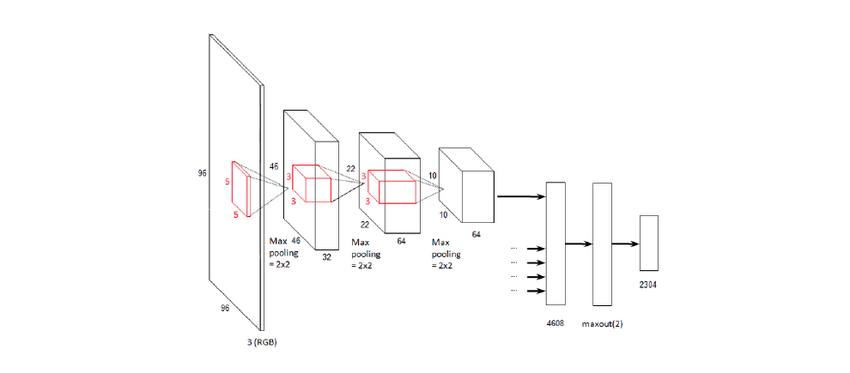
\includegraphics[width=1\textwidth]{figures/chapter-2/convnet.png}
	\caption{Convolutional Neural Network}\label{fig:convnet}   
\end{figure}
A convolutional neural network or \emph{convnet} (illustrated in figure \ref{fig:convnet})is a special kind of feed-forward neural network whose architecture is designed to exploit the principle of locality in the data. This is normally achieved by alternating \emph{convolutional layers} and \emph{pooling layers}. The convolutional layers run a filter or \emph{kernel} across the their input layer which performs an image convolution and can be thought of a way to detect features (such as edges) in the image. The pooling layers usually perform an aggregation (such as taking the maximum of multiple values) over the previous layer to reduce its dimensionality on focus on the salient features.  

While convnets are particularly useful in computer vision and represent the state-of-the-art, for instance, in image classification, they can also be applied in other fields in which the data expresses some principle of locality such as natural language processing. 

\paragraph{Recurrent Neural Networks} In contrast to FFNNs and convnets for which the information flow is strictly uni-directional, recurrent neural networks (RNNs) are characterised by the existence of feedback loops that allows the outputs of a unit in layer $L_i$ to be process as input by any other layer $L_j$, even if $i \geq j$.

This allows the network to learn and store an internal state which can be conceptualised as memory. Such a memory enables the network to effectively deal with sequences of data such as time-series values, natural language, or even acoustic signals like music. 

\begin{wrapfigure}{r}{0.5\textwidth}
	\centering
	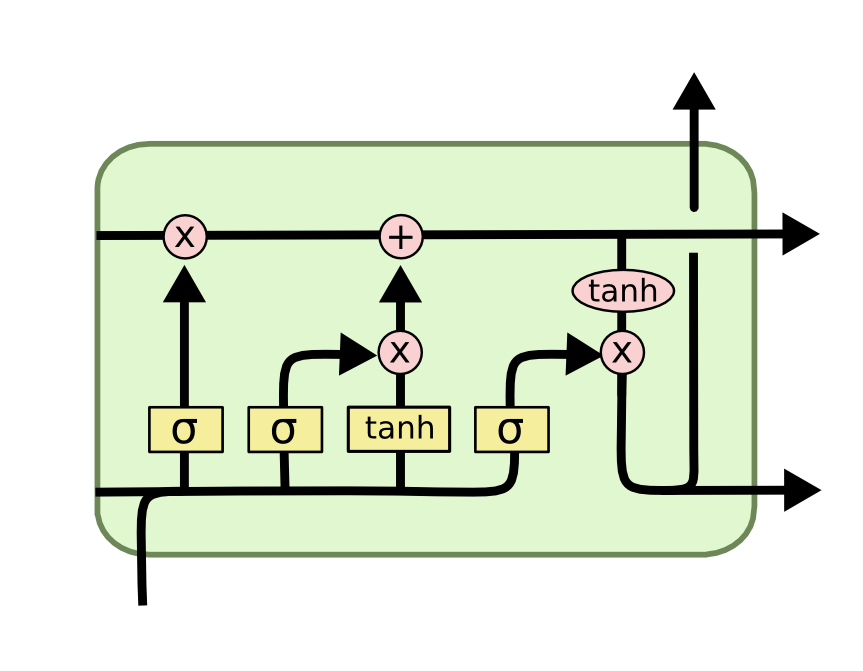
\includegraphics[width=0.5\textwidth]{figures/chapter-2/lstm.png}
	\caption{LSTM}\label{fig:lstm}   
\end{wrapfigure}

In spite of the benefits the recurrent architecture of the network provides, it also introduces a number of computational challenges such as the so called \emph{vanishing gradient problem} which stems from the additional distance the gradient is backpropagated (see next section % TODO Reconsider training section. Should it come before? 
) through the computation graph of the network. In order to circumvent this problem, a number architectures has been proposed for individual cells within the RNN, most notably \emph{long short-term memory} (LSTM) cells and \emph{gated recurrent units} (GRUs). Since RNNs are not of primary interest for the models we investigate for counterfactual inference, the detailed mechanics for these cells are outside the scope of this dissertation.  On a conceptual level, however, LSTM cells address the vanishing gradient problem by utilising a number of \emph{gates} (as illustrated in figure \ref{fig:lstm}) that allow the cell control how the gradient is propagated through the cells, effectively allowing it to decide when to store and when to reset (i.e. forget) its internal state.

Today for many problems in machine learning, RNNs represent the state-of-the-art when dealing with sequential data such as natural language and time-series. 

\subsection{Training}\label{sec:training}
Training a neural network refers to the process of fitting the parameters of the model (i.e. the weights and biases for each cell) to the training data with respect to a given objective function. 

\paragraph{Objective Function}
\begin{wrapfigure}{r}{0.4\textwidth}
	\centering
	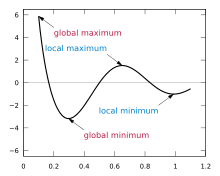
\includegraphics[width=0.4\textwidth]{figures/chapter-2/local-minima.png}
	\caption{Local Minima}\label{fig:local-minima}   
\end{wrapfigure}

The objective function (also called \emph{loss function} or \emph{error function}) defines a performance metric for the model. It is the goal of the training procedure to infer appropriate parameters for the model that maximise its performance (i.e. minimise its loss). 

Figure \ref{fig:local-minima} illustrates this concept by depicting the graph of an objective function $f$ that takes a one-dimensional input (real numbered scalar). As we can see, the function possesses multiple extreme values -- in particular one local minimum at $x = ?$% TODO add proper position
and a global minimum at $x = ?$. % TODO add proper position.  % IMPORTANT!!! GRAPH Add the appropriate positions


In cases where an algebraically obtained closed-form solution for the minimum is not feasible or too computationally expensive, the minimum is often obtained by optimisation algorithms (see below). Since these algorithms often operate in a \emph{greedy} manner, i.e. by a applying series of local operations that has no knowledge about the global surface of the function, we are facing the potential problem of only finding a local optimum but missing out the global one. As a consequence, it is desirable to use convex objective functions that, by definition, only have one (global) optimum. 

The actual loss function is dependent on the problem task and can be derived by a maximum likelihood estimation (MLE). For regression tasks, a common choice is the mean squared error between the prediction $\hat{Y}$ and the actual output value $Y$ defined as 


\begin{align} 
L_{MSE}(w,b) = \frac{1}{n} \sum_{i=1}^{n}(\hat{Y}_i - Y_i)^2.
\end{align} 
For (binary) classification problems we typically use the cross-entropy
\begin{equation}
	L_{CE}(w,b) = - \frac{1}{n} \sum_{i=1}^{n} (Y_i \log \hat{Y}_i + (1 - Y_i) \log 
	(1- \hat{Y}_i)
\end{equation}
as loss function. 

\paragraph{Gradient Descent} We typically make use of an optimisation algorithm that tries to minimise the output of our loss function by capturing to what extend our predictions differ from the target values. A widely used example is \emph{gradient descent} which is an iterative optimisation algorithm that can be used to find a minimum value of a function. Gradient descent repeatedly computes the gradient of the loss function at the current position and subtracts a proportion of the gradient from it until the gradient converges towards zero (which is the case at a minimum) or a stopping condition is satisfied. Intuitively, the subtraction of the gradient can be conceptualised by taking iterative steps in the direction of the steepest descent until a minimum value is reached. 
Formally, we are looking for $x = \text{argmin} f(x)$ by iteratively computing

\begin{equation}	
	\label{eq:gradient-descent-update}
	x_{n+1} = x_n - \alpha \cdot \nabla f(x_n),
\end{equation}
where $x_i$ refers to our position at iteration $i$ and $\alpha \in \mathbb{R}^+$ is a parameter called the \emph{learning rate} that defines the step size of our descent. Choosing an appropriate learning rate expresses a trade-off between reducing the number of required iterations (high learning rate) and a making sure the function converges and does not "overshoot" the actual minimum $x^*$ causing the algorithm to potentially oscillate around the desired optimum. Consequently, it is often desirable to use an \emph{adaptive learning rate} instead, i.e. making $\alpha: \mathbb{N} \rightarrow \mathbb{R}^+$ a function dependent on the current iteration $i$. 

There two main types of gradient descent: \emph{batch gradient descent} computes the gradient for entire dataset before applying an update rule as defined in equation \ref{eq:gradient-descent-update} which is most exact but computationally expensive as the algorithm has to iterate through all $n$ data points in the dataset before applying a single update. In contrast, \emph{stochastic gradient descent} computes the gradient of a random (hence the name) sample and applies an update according to this sample alone which is less computationally expensive. The choice between batch gradient descend and stochastic gradient descend therefore represents a trade-off between accuracy and computational costs. In addition to this dichotomy, there exists a hybrid variation called \emph{minibatch gradient descent} which computes the gradient on a batch which is a subset of the entire dataset. 

\paragraph{Backpropagation} For gradient-based optimisation algorithms it is mandatory to compute the partial derivatives of the objective function $L$ with respect to any weight $w$ or bias $b$ in the neural network that needs to be learnt. In a deep neural network with multiple hidden layers this can be a complex task as the change of a weight influences the outcome (and therefore the loss function) only indirectly by propagating its change through subsequent layers. 

The \emph{backpropagation algorithm} \cite{backprop1} introduces an efficient method to compute the partial derivatives. It conceptualised the network as a concatenation of functions and is based on the simple idea of repeatedly applying the \emph{chain rule} known from calculus to compute the partial derivatives with respect to each parameter (weights and biases) of interest. 

%\begin{wrapfigure}{r}{0.6\textwidth}
%	\centering
%	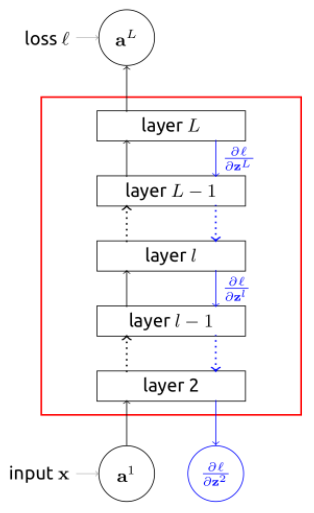
\includegraphics[width=0.6\textwidth]{figures/chapter-2/backpropagation.png}
%		\caption{Backpropagation}\label{fig:backpropagation}   
%\end{wrapfigure}
\begin{figure}[h]
	\centering
	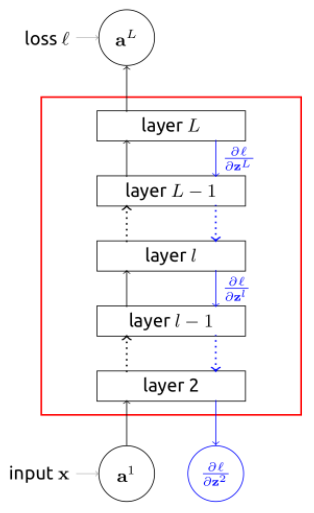
\includegraphics[height=0.5\textwidth]{figures/chapter-2/backpropagation.png}
	\caption{Backpropagation}\label{fig:backpropagation}   
\end{figure}


The training is then executed in two alternating phases that are illustrated in figure \ref{fig:backpropagation}: In the \emph{forward pass} the inputs are propagated through the network from the input layer through the hidden layers until a predicted outcome $\hat{Y}$ is available in the output layer. Using the predicted outcome $\hat{Y}_i$, the actual outcome $Y_i$, and the loss function $L$ we are able to compute a loss \emph{l}.
In the second phase -- the \emph{backward pass} the partial derivatives are computed for the weights and biases of each unit all the way back until the first layer after the input layer. 

Once the partial derivatives are computed, we can update each parameter according to our optimisation algorithm, for instance by applying the update rule defined in equation \ref{eq:gradient-descent-update}. 
The backpropagation algorithm therefore represents an effective technique to compute the gradient of the loss function with respect to the different parameters and is considered an essential part of the training of neural networks. 


\subsection{Dropout} \label{sec:dropout}
As described in section \ref{sec:regularisation}, regularisation is an important concept in machine learning in order to avoid overfitting the training data. While in theory, a traditional approach like \emph{l1} (lasso) and \emph{l2} (weight-decay) regularisation are conceivable, a number of regularisation techniques have been proposed that are specific to the mechanics of neural networks. 

One of the most-used approaches is called \emph{dropout} and was proposed by \citedate{dropout} in 2014. The basic idea is that during training every neuron is kept active only with a certain probability $p$. Conversely, with a probability of $1-p$ it is masked out and represents an output of zero. Intuitively, this prevents the network from becoming too dependent on a particular neuron as it is forced to learn an alternative representation when the neuron is disabled. As a consequence, the network learns a representation that generalises better giving dropout a regularising influence on the network. Similar to the regularisation hyper-parameter $\lambda$ described earlier, the dropout probability $p$ represents a hyper-parameter that has to be chosen appropriately.
\begin{figure}[h]
	\centering
	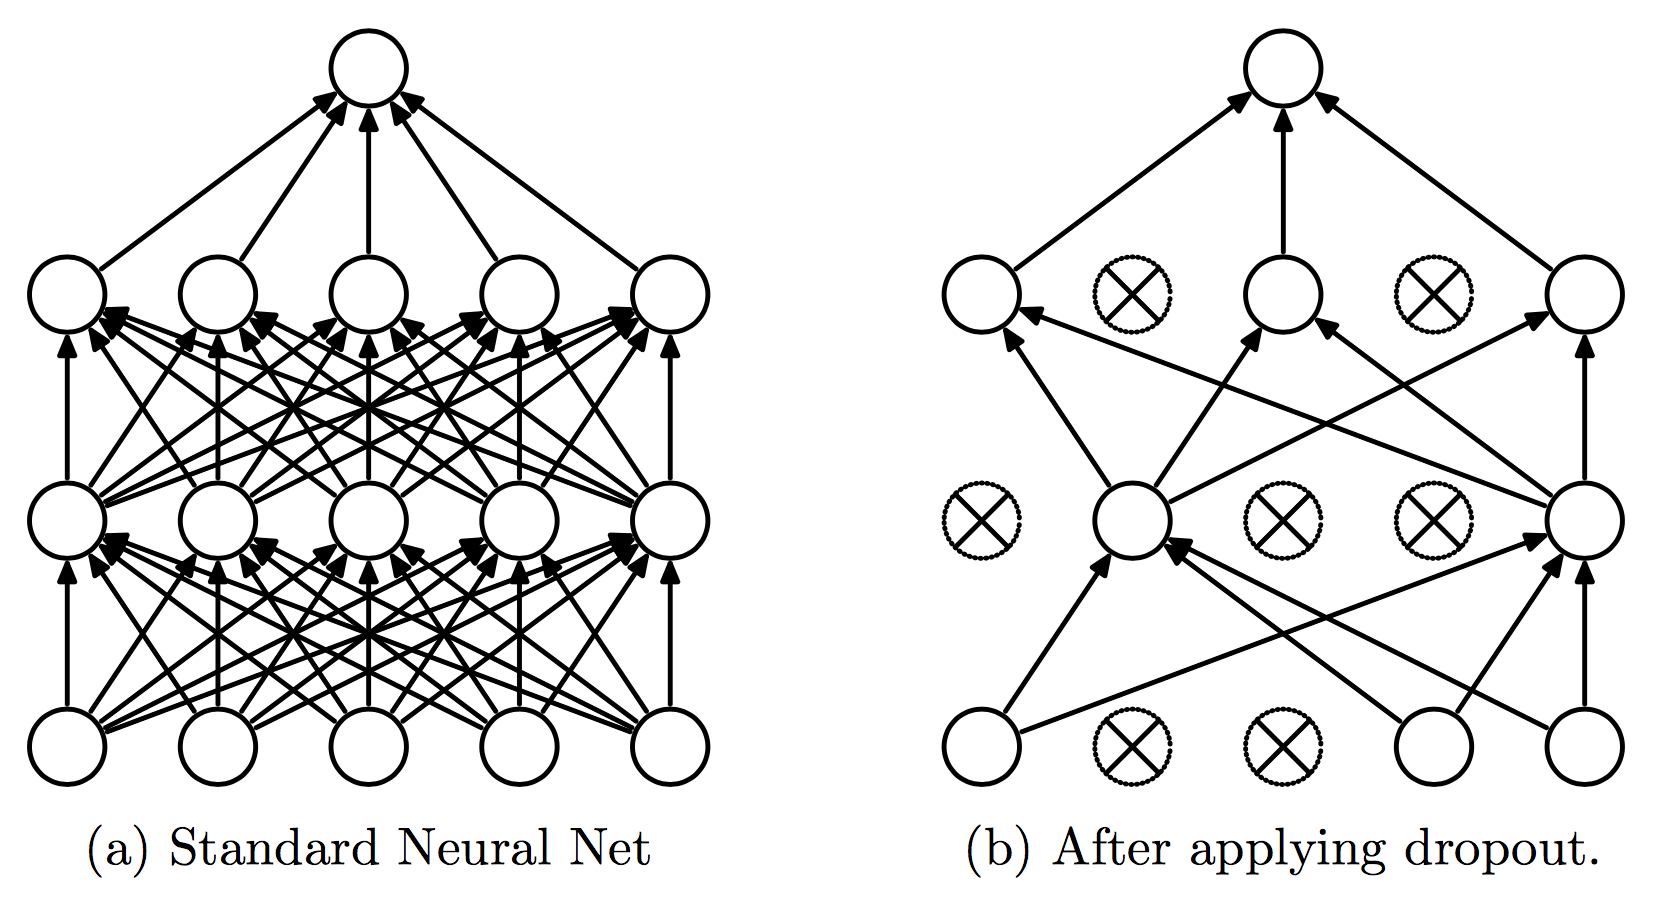
\includegraphics[width=0.8\textwidth]{figures/chapter-2/dropout.png}
		\caption{Dropout}\label{fig:dropout}
\end{figure}


Figure \ref{fig:dropout} illustrates this the concept of dropout: The original network (left side) is thinned out by the dropout resulting in the network on the right side. 

Today, dropout represents the de-facto standard for regularising neural networks and preventing them from overfitting. 


\subsection{Multi-Task Learning}
Neural networks are typically used to perform a single task that is formalised by minimising an appropriate objective function. However, sometimes it is desirable to train the network on multiple (related) tasks simultaneously. 

% GRAPH Cite Hinton % CITE Sebastian Ruder
\begin{wrapfigure}{r}{0.4\textwidth}
	\caption{Multi-Task Learning}\label{fig:multitask-learning}   
	\centering
	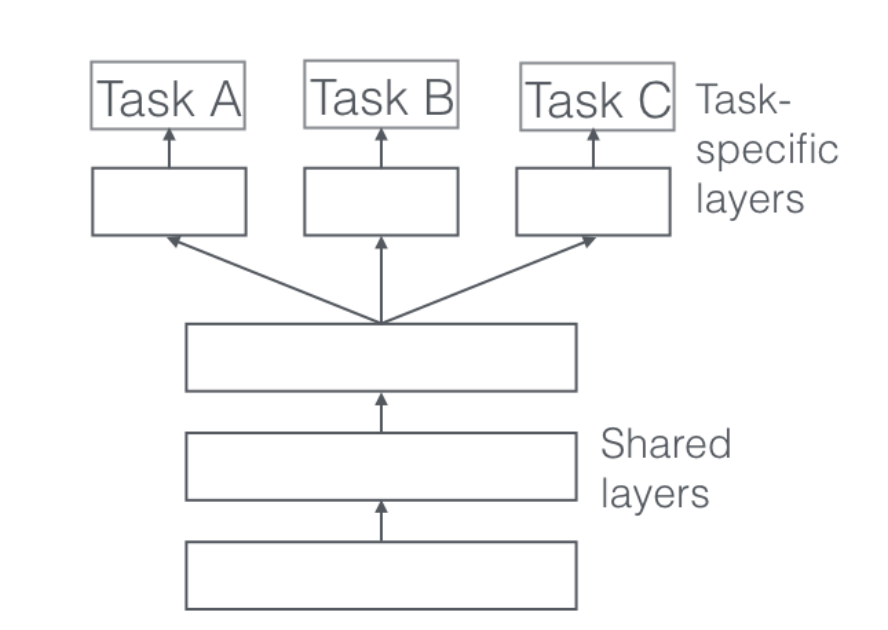
\includegraphics[width=0.4\textwidth]{figures/chapter-2/multitask-learning.png}
\end{wrapfigure}
As illustrated in figure \ref{fig:multitask-learning}, such a multi-task neural network is characterised by a number of layers that are shared between all tasks and a number of layers that are task-specific. Each task typically provides its own objective function which is optimised jointly with the objective functions of the other tasks. 

Multi-task learning can have a variety of desirable properties: Firstly, multi-task neural networks are typically less prone to overfitting as the shared layers have a regularising effect on the network forcing it to learn a shared representation among all tasks. Moreover, they allow influencing the way a task is learnt on a fine-grained level by introducing inductive biases \cite{inductive-bias} that are provided by the other tasks. This means that we can make a primary task more inclined towards considering related sub-tasks. 

As an example for multi-task learning, we consider training a spam classifier for emails. Different users might have distinct distributions over the features of emails they receive due to factors such as language, age, and their interests. Therefore, we can conceptualise the individual classifiers as a number of different tasks. Despite their differences these tasks are highly related allowing us to treat the classifier as a multitask-learning problem. Ideally, the shared layers would learn common concepts of the characteristics of spam emails whereas the individual task-specific layers would take into account the specific characteristics of the user. 

% ... "Bias-free learning is impossible; much of the power of an inductive learner follows directly from the power of its inductive bias [Mitchell 1980]."

% CITE Sebastian Ruder
% CITE http://www.cs.cornell.edu/~caruana/mlj97.pdf




\subsection{Model Selection and Architecture Learning} 
In section \ref{sec:nn-types} we introduced the main types of neural networks, each suitable for different kinds of tasks. However, even after selecting a specific type, there are still a number of architectural considerations that influence the performance of the model. These considerations represent model-level hyper-parameters that are normally defined a-priori and have to be chosen in addition to the hyper-parameters that we already discussed in the previous sections (i.e. the learning rate $\alpha$, the dropout probability $p$, and the type of activation function $\phi$). The following lists such model-level hyper-parameters and how they might affect the network. 

\subsubsection{Model Hyperparameters}
\paragraph{i) Number of layers} The number of layers (or \emph{depth}) of the network is a key design decision for the model's architecture and greatly influences its performance. In general, a greater number of layer results in a more complex model with higher variance increasing its ability to capture complex non-linear dependencies. On the flip side, % TODO Can I say this? 
it also increases the risk of  over-fitting the training data and therefore requires stronger regularisation. From a practical perspective, a higher number of layers also causes the model to be more computationally expensive and require a larger memory to store the trained parameters. 

Consequently, the number of layers corresponds to the classical trade-off between bias and variance discussed in section \ref{sec:regularisation} and thus depends on the amount of available data, the degree of regularisation, and computational considerations. 


\paragraph{ii) Number of units per layer} In addition to the number of hidden layers, we need to decide on an appropriate number of units per hidden layer (network \emph{width}). The decision follows a similar rationale to the number of layers: A high number of units per layer increases the variance of the model allowing it to accommodate more complexity while increasing the risk of over-fitting.  


\subsubsection{Hyper-Parameter Optimisation}
In contrast to ordinary parameters (i.e. weights and biases) of the model, hyper-parameters are typically not learnt during training but need to be chosen a-priori. However, there are three main techniques for deriving suitable hyper-parameters:

\paragraph{i) Grid Search} The most basic form of finding appropriate hyper-parameters is to perform a \emph{grid search}. This means iteratively trying a set of candidate values for each hyper-parameter leading to an exhausting search over the space of potential hyper-parameters. After each iteration, the model is trained and then evaluated on a dedicated \emph{cross validation set} which is a subset of the entire dataset disjoint from the training and test set. The set of hyper-parameters with the maximum performance is ultimately chosen for the model.   
While this approach is feasible for a small search space, it becomes computationally challenging if the space of potential hyper-parameters is large. 

\paragraph{ii) Random Search} An alternative to grid search that is computationally less expensive is \emph{random search}: Instead of trying every possible hyper-parameter in the search space exhaustively, this approach randomly samples hyper-parameters from the search space a fixed amount of times. 

\paragraph{iii) Bayesian Optimisation} Bayesian optimisation \cite{bayesian-optimisation} of hyper-parameters uses \emph{Gaussian processes} (GPs) to map a distribution over the hyper-parameters to an (initially unknown) objective function of our model that we want to optimise. We are trying to evaluate the search space of hyper-parameters in a way, that provides the maximum insight about the objective function and its potential minimum.  This is achieved by using concepts of Bayesian inference, i.e. obtaining a \emph{posterior probability} by updating our previous beliefs (\emph{prior}) with evidence following \emph{Bayes' Rule}. 

In practice, it has been shown that Bayesian optimisation has the potential to outperform competing approaches (such as grid search) while requiring a fewer number of iterations \cite{bayesian-optimisation-results}. Nevertheless, due to the curse of dimensionality, in most settings the process is still considered computationally expensive. 


%\subsubsection{Architecture Learning}
%Nevertheless, a number of approaches to automatically deriving suitable architectures has been proposed by a concept called 
%
%It is difficult to derive proper architecture. 
%What's the right number of hidden layers? What's the right number of hidden units per layer, etc? 
%Different approaches to architecture learning. Optimal Brain Surgeon/Damage. GridSearch, RandomSearch, Bayesian Optimisation.

%\subsection{Challenges}
%Computational complexity
%Lots of parameters (high memory)
%Lots of hyper-parameters 
%Low Understandability. Some people confuse softmax with confidence. 
%
%Lorem ipsum dolor sit amet consectetur, adipiscing elit mus neque montes, suspendisse et sociis vestibulum.

\section{Counterfactual Inference} \label{sec:counterfactual-inference}

\subsection{Motivation}
% TODO Check overlap with Introduction section
The concept of causality represents the foundation of disciplines such as reasoning and logic. To some extent, most scientific research can be considered as an attempt to investigate the causal relations within different concepts in order to understand what \emph{cause of actions} results in  what \emph{effect}.

Despite its importance, the study of causality is inherently difficult since most phenomena are governed by a complex network of interdependencies and correlations making it almost impossible to identify pure causal relations such as $A \rightarrow B$.  

In practice, causal inference is often performed in the scope of observational studies that try to investigate the effect $Y$ a certain intervention or treatment $T$ has on a given context $X$. For instance, we consider a medical setting in which such a study investigates how the blood pressure ($Y$) of a given patient ($X$) changes after being administered a medication ($T$) of interest.

When considering causal relations within the data, we are often interested in answering \emph{counterfactual questions} such as "What would have happened if a different action had been taken?”. In order to understand the importance of such counterfactual questions, we have to introduce the concept of the \emph{individualised treatment effect} or ITE.

The ITE is a quantity that is defined as the difference between the observed or \emph{factual outcome} and the unobserved or \emph{counterfactual outcome}. Intuitively, this means that the ITE tells us how the outcome would change depending on whether or not we perform % LANG is this the proper verb? 
the intervention of interest. 
As a consequence, if we had access to this quantity, we could immediately decide which outcome (treated or untreated) is closer to the desired effect. In our medical context mentioned above, having access to the ITE of a medication on a given patient would be a crucial benefit during treatment planning. 

Unfortunately, by its very definition it is infeasible to obtain the ITE for any real-world dataset: An observational study can only give us access to the observed outcome -- the counterfactual outcome is never available. 
% GRAPH Make graph pretty
\begin{table}[]
	\centering
	\caption{Counterfactual Inference Example}
	\label{tab:counterfactual-inference-motiviation}
	\begin{tabular}{@{}lllll@{}}
		\toprule
		X & T & $Y^{(1)}$ (treated) & $Y^{(0)}$ (untreated) & ITE \\ \midrule
		1 & 0 & ? & 100 & 100 - ? \\
		2 & 1 & 110 & ? & 110 - ?  \\
		3 & 1 & 98 & ? &  98 - ?  \\
		4 & 0 & ? & 101 & 101 - ? \\
		5 & 0 & ? & 107 &  107 - ? \\
		6 & 1 & 99 & ? &  99 - ?\\ \bottomrule
	\end{tabular}
\end{table}

Consider the example illustrated in table \ref{tab:counterfactual-inference-motiviation}. We are given a dataset of six subjects $X \in \{1, 2, 3, 4, 5, 6\}$ half of which received a treatment indicated by $T=1$ while the other half did not receive it (i.e. $T=0$). Depending on their treatment assignment, we can either directly observe the treated outcome $Y^{(1)}$ or the untreated outcome $Y^{(0)}$ but never both, making it impossible to calculate the ITE. 


As a consequence, the objective of counterfactual inference is to \emph{estimate} the unobserved outcome which allows us to estimate the ITE, helping us make informed decisions regarding the treatment assignment. 

% TODO Rephrase as this overlaps with the intro!
Finally, it can be said that the applications of counterfactual inference are ubiquitous and highly relevant to a variety of fields including treatment-planning in healthcare, policy-making for organisations, and even ad-placement for online platforms. 
%As a consequence, research in this field can have a significant impact on a number of disciplines and potentially affect many people’s lives by helping important institutions, governments, and industries to make more informed decisions.


\subsection{Formalisation}
We represent each subject $i$ in our population  with a $d$-dimensional feature vector $X_i \in \mathcal{X}$, and two \emph{potential outcomes} $Y_{i}^{(1)}, Y_{i}^{(0)} \in \mathbb{R}$ (following \cite{potential-outcomes}) which are drawn from a distribution
\begin{equation}
 (Y_{i}^{(1)}, Y_{i}^{(0)}) \mid X_i = x \sim \mathbb{P}(\cdot \mid X_i = x)
 \end{equation}.
This way, the \emph{individualised treatment effect} for subject $i$ can be expressed as 

\begin{equation}
T(x) = \mathbb{E}[Y_{i}^{(1)} - Y_{i}^{(0)} \mid X_i = x] . \label{eq:ite}
\end{equation}

Given this definition, the objective is to approximate the function $T(x)$ using an observational dataset $\mathcal{D}$ consisting of $n$ independent samples. 

Each sample is comprised of a tuple $ \langle X_i, W_i, Y_{i}^{(W_i)} \rangle$, where $X_i$ represents the subject's features, $W_i \in \{0,1\}$ the treatment assignment indicator, and $Y_{i}^{(W_i)}$ and $Y_{i}^{(1 - W_i)}$ the respective \emph{factual} and \emph{counterfactual} outcome. 

The treatment assignment (covered in detail in section \ref{sec:propensity-score}) is modelled as a random variable depending on the subjects' features, i.e. $W_i \not \perp X_i$. The assignment reflects a domain-specific policy which can be captured in terms of the probability $p(x) = \mathbb{P}(W_i = 1 \mid X_i = x)$ called the \emph{propensity score}.

The objective of counterfactual inference is to fit a function to the observed data $\mathcal{D}$ in order to estimate the individualised treatment effect. A variety of models and approaches has been proposed as discussed in detail in section \ref{sec:status-quo}.
% TODO What about how to estimate the ITE?  


\subsection{Counterfactual Inference vs. Supervised Learning} \label{sec:cfi-vs-supervised-learning}
When fitting a function to estimate the ITE we could technically use any kind of model fitting approach. However, it is imperative to understand how the task of estimating the ITE using counterfactual inference is fundamentally different from a standard \emph{supervised learning problem} in machine learning.

% GRAPH Create graph that illustrates the example. ALSO, see critical section below
\begin{wrapfigure}{r}{0.6\textwidth}
	\centering
	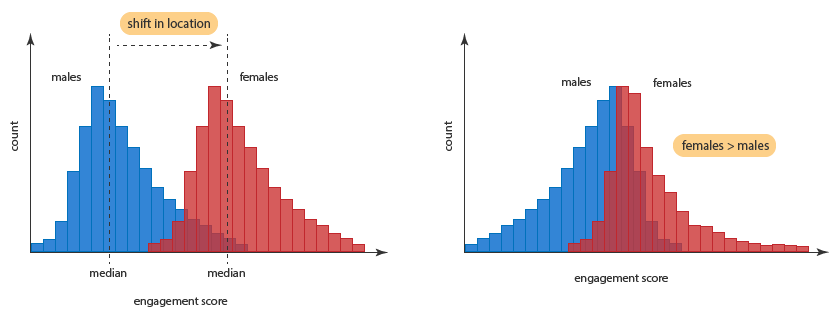
\includegraphics[width=0.6\textwidth]{figures/chapter-2/counterfactual-vs-supervised-learning.png}
	\caption{Counterfactual Inference vs. Supervised Learning}\label{fig:counterfactual-inference-vs-supervised-learning}   
\end{wrapfigure}


The problem requires making inferences on a set of counterfactual samples using a set of factual
samples. These two quantities, however, normally do not follow the same probability distribution. In fact, this would only be the case if the treatment was assigned randomly with an equal chance of $p = 0.5$ for which we could treat the problem as a supervised learning problem.  In reality, the treatment assignment is not random but reflects a particular domain-specific policy (see section \ref{sec:propensity-score}). 

%Consider the following example illustrated in figure \ref{fig:counterfactual-inference-vs-supervised-learning}: A doctor is treating patients with ... 
% CRITICAL!!! GRAPH Write proper example that corresponds with figure
%For example, one may be interested to know the consequences of smoking or the consequences of going to university. The people 'treated' are simply those—the smokers, or the university graduates—who in the course of everyday life undergo whatever it is that is being studied by the researcher. In both of these cases it is unfeasible (and perhaps unethical) to randomly assign people to smoking or a university education, so observational studies are required. The treatment effect estimated by simply comparing a particular outcome—rate of cancer or lifetime earnings—between those who smoked and did not smoke or attended university and did not attend university would be biased by any factors that predict smoking or university attendance, respectively. PSM attempts to control for these differences to make the groups receiving treatment and not-treatment more comparable. (WIKIPEDIA)

Formally, we are inferring the outcomes over a counterfactual dataset $CF = \{(x_i, 1 - t_i) \}^{n}_{i=1}$ which is distributed according to some probability distribution $CF \sim P^{CF}$ using outcomes that were estimated over a factual dataset $F = \{(x_i, t_i) \}^{n}_{i=1}$ with $F \sim P^{F}$ where $P^{CF} \neq P^F$. We are a dealing with a \emph{covariate shift} which is often encountered in domain adaptation problems (\cite{domain-adaptation}).

Consequently, if we simply treated the treatment assignment as an ordinary input feature in our dataset, we might be introducing significant biases caused by the covariate shift.  Therefore, it can be said that when performing counterfactual inference, we have to take specific measures in order to ensure a meaningful estimation of the ITE that overcomes the covariate shift problem caused by the selection bias of the treatment assignment. 


\subsection{Treatment Assignment and Propensity Score} \label{sec:propensity-score}
Whether or not a context receives the intervention typically depends on an underlying domain-specific policy. Such policies can be well-defined in  a rule-based setting like 
\begin{equation}
\text{age}(x) < 45 \wedge \text{HIV}(x) = \text{negative} \rightarrow T_x = 0
\end{equation} 
or less rigorous and simply reflect a decision maker's informal intuition. In both cases, it is important to understand that -- even though we might not be able to comprehend the policy -- the decision is not made randomly but depending on the concrete features of the context or subject. 

In the scope of counterfactual inference, we typically do not assume any kind of control or knowledge of the policy. Instead, we model a subject's inclination to receive the treatment as a random variable called \emph{propensity score} defined as 

\begin{equation}
p(x) = \mathbb{P}(W_i = 1 \mid X_i = x)
\end{equation}
where $X_i$ denotes the subject's features and $W_i$ the treatment assignment with $W_i \not \perp X_i$ (the treatment assignment is not independent from the features). 

While the propensity score is defined for each subject individually, we are sometimes also interested in the \emph{average propensity score} 

% TODO Is this the same as average treatment assignment? 
\begin{equation}
	\mathbf{B} = \frac{1}{n} \cdot \sum \limits_{{i=1}}^{n}  \mathbb{P}(W_i = 1 \mid X_i)
\end{equation}

for a given dataset yielding an estimate of the selection bias of the policy. 

\subsection{Estimating Treatment Effects} \label{sec:status-quo}
% TODO Check out Ahmed's related work sections
A number of different methods and models has been proposed in order to estimate treatment effects. 

\paragraph{Propensity Score Matching} Early works were not able to estimate the ITE directly but focuses on the \emph{average treatment effect} or ATE instead, defined as the expected value of all individualised treatment effects

\begin{equation}
\text{ATE} = \mathbb{E}[T(x)]
\end{equation}
over a population of interest using a method called \emph{propensity matching}. % CITE propensity matching (Rubin, 2011; Austin, 2011; Abadie & Imbens, 2016; Rosenbaum & Rubin, 1983; Rubin, 1973).

Propensity score matching  can be summarised as follows: First, we estimate the propensity scores of each subject in the dataset. This is achieved by training a classifier, typically logistic regression or random forests, on the dataset using the treatment assignment as target value that we want to predict. Secondly, we match each subject in the control group (i.e. the subset of untreated patients in the dataset) to one or more (e.g. by using k-nearest-neighbour) corresponding subjects in the treatment group that most closely resemble the untreated subject. Finally, we are able to estimate  the average treatment effect by computing the average of the differences between the matched subjects. 

However, it has been pointed out (\cite{propensity-score-matching-sucks}) that there are a number of limitations and challenges for this approach. For instance, in a randomised trial (i.e. $p =0.5$) the propensity scores of any two subjects will roughly be equal while their features can be significantly different resulting in misleading predictions. (\cite{propensity-score-matching-sucks}) goes as far as saying that propensity scores should not be used for matching at all. 

In addition, propensity score matching is limited to estimating the \emph{average }treatment affect and does not allow us to compute the more fine-grained ITE. 


% Classical works have focused on estimating “aver- age” treatment effects through variants of propensity score matching (Rubin, 2011; Austin, 2011; Abadie & Imbens, 2016; Rosenbaum & Rubin, 1983; Rubin, 1973). More recent works tackled the problem of estimating “indi- vidualized” treatment effects using representation learn- ing (Johansson et al., 2016; Shalit et al., 2017), Bayesian inference (Hill, 2012), and standard supervised learning (Wager & Athey, 2015).
%

\paragraph{Direct Modelling}
Despite the differences of counterfactual inference to supervised learning, it has been attempted model the ITE directly for instance using K-nearest-neighbour matching, or more recently using random forests (\cite{random-forests}) and neural networks (\cite{sontag-direct-modelling}) that are treating the treatment assignment as a feature.

One way to address the problem of covariate shift caused by the selection bias described in section \ref{sec:cfi-vs-supervised-learning}, is to introduce a dedicated term in the objective function that penalises the imbalance between the factual and counterfactual distributions.  


\paragraph{Representation Learning} \label{sec:representation-learning}
Most recently, deep neural networks have been applied to the problem of counterfactual inference resulting in promising first results. 

One of the current state-of-the-art methods called \emph{balancing neural network} (BNN) treats the task as a problem in \emph{representation learning} (\cite{sontag-paper}).

The approach is based on the concept of learning balanced representations for the treated and untreated subjects in the dataset such that the discrepancy between the distributions of the factual and counterfactual outcomes is reduced. 

\begin{figure}[h]
	\centering
	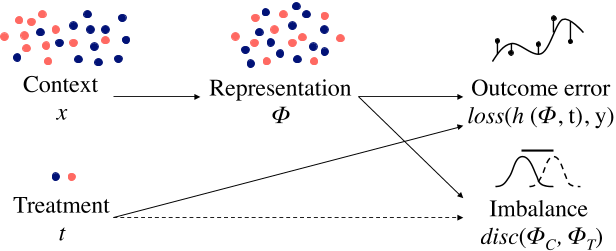
\includegraphics[width=0.8\textwidth]{figures/chapter-2/balanced-representations.png}
	\caption{Learning Balanced Representation for Counterfactual Inference}\label{fig:balanced-representations}
\end{figure}

Concretely, they propose an architecture for feed-forward neural networks (illustrated in figure \ref{fig:balanced-representations-architecture}) in which the first $d_r$ hidden layers are responsible for learning a balanced representation $\Phi$ which is then processed in the remaining $d_o$ hidden outcome layers. 
The imbalance of the representation is minimised in terms of a function \emph{disc} whereas the outcome is optimised using the objective function 

\begin{equation}
	\text{loss}(h(\Phi, t), y) = \frac{1}{n}\sum_{i=1}^{n} \mid h(\Phi(x_i)), t_i), - y_i^{F} \mid
\end{equation}

that computes the absolute error between the prediction of the learnt hypothesis function $h$ on the inputs $x_i$ represented in terms of the learnt representation $\Phi$ and the actual (factual) outcome $y_i^F$. 

\begin{figure}[h]
	\centering
	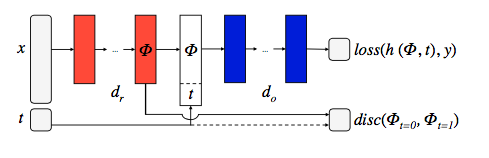
\includegraphics[width=0.8\textwidth]{figures/chapter-2/sontag-architecture.png}
	\caption{Architecture for Balanced Representations}\label{fig:balanced-representations-architecture}
\end{figure}

Their method consistently outperformed competing approaches and can be considered state-of-the-art. 


\paragraph{Deep Neural Networks} 
Despite the recent successes of deep neural networks in many problem areas, only limited research has been done on using them for the task of causal inference. However, the previous example of representation learning \cite{sontag-paper}, indicates promising first results and demonstrates that neural networks can be highly suitable for the task. 
 
This thesis deals with the questions of how to improve the state-of-the-art in counterfactual inference using deep neural networks. In the following chapters, we propose a novel architecture for neural networks that conceptualises the problem as a multi-task learning problem, we introduce a propensity-based dropout scheme for regularisation and overcoming the selection bias, and present an efficient way to infer suitable hyper-parameters for the model. 


%\subsection{Challenges}
%How to improve accuracy? 
%What are good architectures? 
%How to train them? 
%Dropout? 



\part{Methodology}
%\begin{savequote}[8cm]
%\textlatin{Jedem Anfang wohnt ein Zauber innne.}
%
%In the core of every beginning lives magic.
%  \qauthor{--- Hermann Hesse's \textit{Stufen}}
%\end{savequote}

\chapter{\label{ch:3-DCNs}Deep Counterfactual Networks} 

%\minitoc

\section{Motivation}
Deep neural networks represent one of the key areas of research in machine learning. They are responsible for a multitude of recent success in various fields such as computer vision and natural language processing. 

Despite their success, only limited research has been done on how to use deep neural networks for the task of counterfactual inference. However, recent results % CITE Sontag
have shown that neural networks can not only provide a valid option worth considering but is actually able to outperform the state-of-the-art. 

Nevertheless, there is a number of open questions when it comes to applying deep neural networks to counterfactual inference. Firstly, we have to deal with the problem of \emph{covariate shift}, i.e. the different distribution of the feature in the factual and counterfactual datasets respectively. Secondly, deep neural networks typically act as a black-box, lacking any kind of understandability or statistical interpretation. % LANG Does the words interpretablity exist? 
In particular, we are not able to provide confidence intervals with the respect to the quality of our prediction. While confidence intervals are a desired feature to have in almost every kind of task, they could be considered of crucial importance for the task of counterfactual inference: We just need to think of a doctor in a hospital who is using our model to generate actionable insights on whether or not to administer a certain treatment to a patient in need. Here, understandability is of key importance since the doctor needs to be able to trust the algorithm and potentially justify her decision that were based on the algorithm. 

In the following, we propose a model that we call \emph{deep counterfactual network} or (DCN) that conceptualises the counterfactual inference as a multi-task learning problem. In addition, we introduce novel dropout scheme that is based on the propensity score and allows a probabilistic interpretation of the model. 
\section{Model Description}
Previous models often followed the approach of \emph{direct modelling} in which a single-output regression model 
\begin{equation}
f: \mathcal{X} \times \{0,1\} \rightarrow \mathbb{R}
\end{equation}
is used to estimate the individualised treatment effect $T(x)$, with $\mathcal{X}$ being the population of contexts. In other words, the treatment assignment $W_i \in \{0,1\}$ for each subject is used as a bivariate input feature of the model. 

  The model is \emph{statistically efficient} in the sense that it makes use of the commonalities between the different response surfaces of the treated and untreated subjects. On the flip side, it sacrifices accuracy as it limits the interaction between the treatment assignment and the other features of the subject, in particular when dealing with  high-dimensional input data where the treatment assignment might simply get lost among the other features. Moreover, if the \emph{response surfaces} of the treated and untreated subjects differ significantly (e.g. features that are relevant to one outcome are are significant for the other outcome and vice versa), the model performs poorly and the consequences can be severe. 

A competing previous approach called \emph{virtual twin} uses two completely separate models to fit the treated and untreated population. % CITE Lu at al. 
While this approach has a high modelling flexibility and expressiveness for both outcomes, it sacrifices its \emph{statistical efficiency} as both outcome models are completely separated and therefore not able to reuse any of the correlations observed in the model for the respective other outcome. 




\begin{figure}[h]
	\centering
	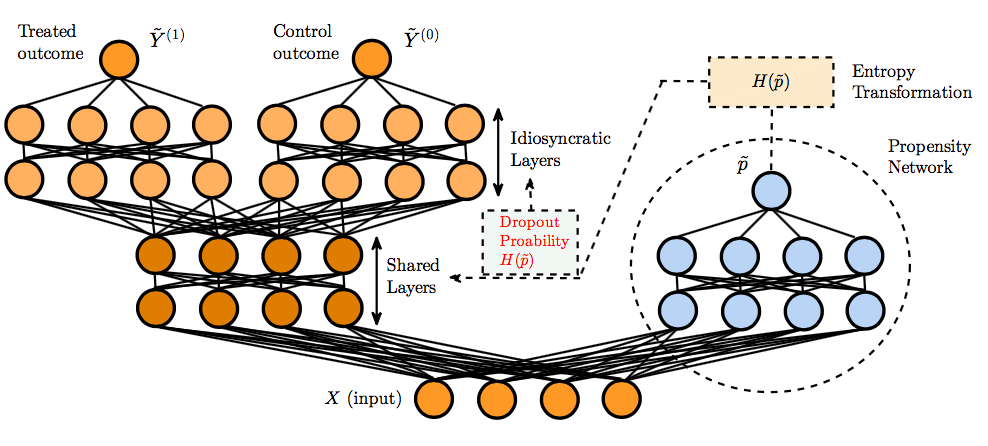
\includegraphics[width=1.0\textwidth]{figures/chapter-3/pbd-architecture.png}
	\caption{Architecture of Deep Counterfactual Networks}\label{fig:dcn-architecture}
\end{figure}

We introduce \emph{deep counterfactual networks} a novel approach to using deep neural networks for the task of counterfactual inference. Our model -- illustrated in figure \ref{fig:dcn-architecture} and described in detail in the following -- conceptualises counterfatual inference as a multi-task learning problem (see section \ref{sec:multi-task-learning}). This way, we achieve  statistical efficiency while at the same time ensuring a high degree of modelling flexibility. 

In addition, we address the  problem of the covariate shift between the factual and counterfactual dataset by utilising a novel propensity-based dropout scheme (see section \ref{sec:propensity-based-dropout}). This way, we are also able to provide confidence intervals for our predictions increasing. 

\subsection{Multi-Task Learning} \label{sec:multi-task-learning}
\emph{Deep counterfactual networks} (DPNs) make use of multi-task learning to learn a \emph{shared representation} for the potential outcomes (treated and untreated) in order to predict the individualised treatment effect $T(x)$. 

Our model, illustrated in figure \ref{fig:dcn-architecture}, consists of two separate networks: A \emph{propensity-network} on the right and a \emph{potential outcomes network} on the left.

The propensity-network represents a standard feed-forward neural network consisting of $L_p$ hidden layers and $h_p^{(l)}$ hidden units for the $l^{th}$ layer. It is trained separately and used to estimate the propensity scores for each sample $(X_i, W_i) \in \mathcal{D}$, thus treating the problem as a binary classification problem with the treatment assignment as target label. 

The \emph{outcome network} uses a multi-task architecture % CITE Collobert & Weston
with $L_s$ \emph{shared layers} (with $h_s^{(l)}$ hidden units in the $l^{th}$ layer) and $L_{i,j}$ \emph{outcome-specific layers} (with $h_{i,j}^{(l)}$ hidden units in the $l^{th}$ layer) for each outcome $j \in \{0,1\}$. This way, we treat the learning of the two outcome response surfaces $\mathbb{E}[Y_i^{(1)} \mid X_i = x]$ and $\mathbb{E}[Y_i^{(0)} \mid X_i = x]$ as two separate but related tasks that are learnt jointly in terms of a multi-task learning problem.

As a consequence, the training data $\mathcal{D}$ obtained from an observational study is separated into two task-specific subsets: a \emph{treated set} $\mathcal{D}^{(1)} = \{i \in \mathcal{D} : W_i = 1\}$ containing all treated subjects, and a \emph{control set} $\mathcal{D}^{(0)} = \{i \in \mathcal{D} : W_i = 0\}$ comprised of all untreated subjects. 

It is the purpose of the shared layers to capture any commonalities between the two outcome surfaces of both tasks. The shared layers also ensure a high level of statistical efficiency as they are able to make use of both datasets $\mathcal{D}^{(0)}$ and $\mathcal{D}^{(1)}$. 

In contrast, the outcome-specific layers allow the model to capture any individual complexity for each response surface. This is achieved by only using the subset $\mathcal{D}^{(j)}$ to learn the response surface $\mathbb{E}[Y_i^{(j)} \mid X_i = x]$, giving us a high level modelling flexibility that ensures accurate predictions even when the response surfaces differ significantly. 

Concluding, treating the problem of counterfactual inference as a multi-task learning problem enables us to train a flexible model that is able to capture potential individual for each response surface while at the same time ensuring an statistically efficient use the entire dataset for any shared complexity. 
	
\subsection{Propensity-based Dropout} \label{sec:propensity-based-dropout}
One of the key challenges of counterfactual inference is the problem of the \emph{covariate shift} (different distribution of the features) between the factual and counterfactual dataset which is caused by the selection bias of the treatment assignment policy.

In our model, we address this issue by applying a special regularisation technique that we will refer to as \emph{propensity-dropout} or PD. Propensity-dropout is based on regular dropout % CITE Hinton
that utilises the individual propensity score of a subject when training the model. In other words, for each individual sample we use a different dropout probability for the nodes in the network calculated as
\begin{equation}
P_{\text{dropout}}(x) = 1 - \frac{\lambda}{2} - \frac{1}{2} \mathbb{H}(\tilde{p}(x))
\end{equation}
where $\tilde{p}$ is the propensity score of subject $x$ as estimated by our \emph{propensity network}, $0 \leq \gamma \leq 1$ is an adjustable parameter (we typically use $\gamma = 1$), and $\mathbb{H}$ with
\begin{equation}
\mathbb{H} = -p \log (p) - (1-p)\log (1-p)
\end{equation}
refers to the entropy % CITE SHANNON
known from information theory. 

Consequently, a sample $x$ with an extreme propensity score ($\tilde{p}(x) = 0$ or $hat{p}(x) = 1$) receives a high dropout probability of $P_{\text{dropout}}(x) = 1 - \frac{\lambda}{2}$ (i.e. typically $0.5$), whereas samples with a balanced propensity score $\hat{p}(x) = 0.5$ receive a low dropout probability $P_{\text{dropout}}(x) = \frac{1}{2} - \frac{\lambda}{2}$ (typically 0).

Intuitively, we want our dropout scheme to mask out hidden units in a way that assigns "simple models" to subjects with very high ($p(x)$ close to $1$) or low  ($p(x)$ close to $1$) propensity scores, whereas we want to assign more "complex models" to subjects that have a balanced propensity score ($p(x)$ close to $0.5$). In other words, the dropout probability will be higher for subjects with potentially unreliable features that belong to an area of small treatment assignment overlap in the feature space. This way, we penalise training sample with extreme propensity scores in order to prevent the network from co-adapting with potentially unreliable samples, allowing the model to generalise better to the actual distribution of features.

%Propensity-dropout represents a conceptual equivalent to propensity-weighting % CITE Abadie and Ibens
%that is applied on regular dropout. % CITE Srivstava et al 
 
Besides its regularising and balancing effect towards the covariate shift introduced by the selection bias, propensity dropout enables us to associate the estimated individualised treatment effects $\tilde{T}(x)$ with a corresponding measure of confidence. This can be achieved by utilising a Monte Carlo propensity-dropout scheme where we draw samples of $\tilde{T}(x)$  for our model. % CITE GAL & Ghahramani
In our model, a sample of $\tilde{T}(x)$  for a subject with features $x$ can be drawn as defined by:
\begin{flalign} % TODO DOUBLE CHECK THESE EQUATIONS!!!!!
	\tilde{p}(x) = f(...f((w_p^{(1)})^Tx)...) \\
	\mathbf{r}_s^{(l)}, \mathbf{r}_{i,0}^{(l)}, \mathbf{r}_{i,1}^{(l)} \sim Bernoulli(1-\frac{\lambda}{2} - \frac{1}{2}\mathbb{H}(\tilde{p}(x))) \\
	\tilde{s}(x) = f(...f(\mathbf{r}_s^{(1)}  \odot (\mathbf{w}_s^{(1)})^T x)...) \\
	\tilde{Y}^{(1)} = f(...f(\mathbf{r}_{i,1}^{(1)}  \odot (\mathbf{w}_{i,1}^{(1)})^T \tilde{s}(x))...) \\
	\tilde{Y}^{(0)} = f(...f(\mathbf{r}_{i,0}^{(1)}  \odot (\mathbf{w}_{i,0}^{(1)})^T \tilde{s}(x))...) \\			
	\tilde{T} = \tilde{Y}^{(1)} - \tilde{Y}^{(0)},
\end{flalign}
where $\mathbf{w}_p^{(l)}, \mathbf{w}_s^{(l)}, \mathbf{w}_{i,0}^{(l)},$ and $\mathbf{w}_{i,1}^{(l)}$ refer to the weight matrices for the $l^{th}$ respective propensity, shared, or outcome-specific layer; $\mathbf{r}_s^{(l)}, \mathbf{r}_{i,0}^{(l)},$ and $\mathbf{r}_{i,1}^{(l)}$ correspond to the dropout masks, and $f: \mathbb{R} \rightarrow \mathbb{R}$ is an arbitrary activation function (e.g. a ReLU or the logistic function). 

\section{Training the Model} \label{sec:dcn-training}
The network is trained in two alternating phases. In each phase, we use either the untreated samples $\mathcal{D}^{(0)}$ or the treated samples $\mathcal{D}^{(1)}$ as our training set to update the weights. 
% TODO Replace with actual algorithm!!!
\begin{figure}[h]
	\centering
	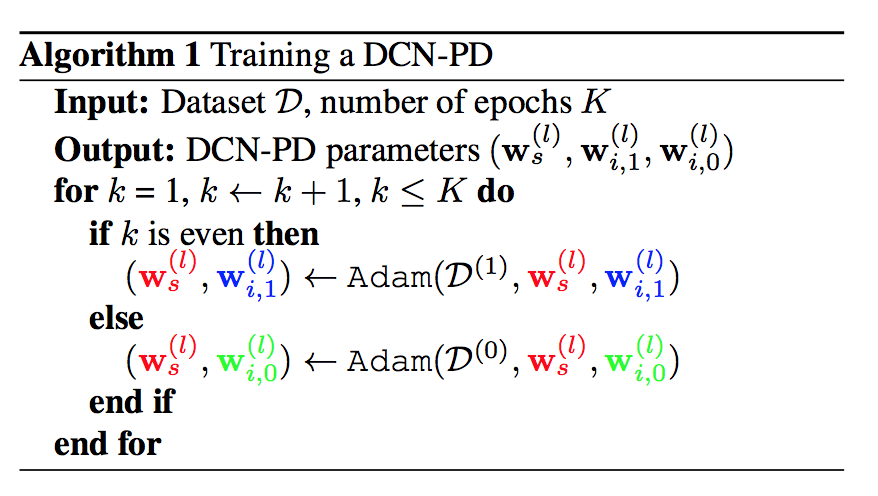
\includegraphics[width=0.6\textwidth]{figures/chapter-3/training-algorithm.png}
	\caption{Training Algorithm}\label{fig:training-algorithm}
\end{figure}
The algorithm is outlined in listing \ref{fig:training-algorithm} and can be described as follows: We train the model by iterating over a total $K$ epochs. In the even epochs ($k \mod 2 = 0$), we use $\mathcal{D}^{(1)}$ to update the weights of the outcome-specific layers of the treated subjects, in the odd epochs ($k \mod 2 \neq 0$) we update the outcome-specific layers of the control subjects. 

\begin{figure}[h]
	\centering
	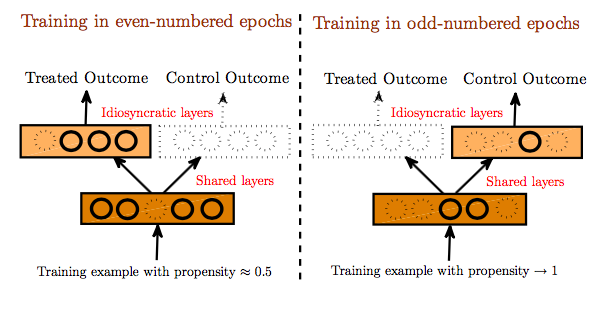
\includegraphics[width=0.8\textwidth]{figures/chapter-3/pbd-training.png}
	\caption{Visualisation of Training Algorithm}\label{fig:dcn-training}
\end{figure}


Note, how the weights of the shared layers are updated in every iteration. In order to update the weights, we are using the \emph{Adam optimiser} with \emph{Xavier initialisation}. % CITE Kingma & Ba
% TODO Consider if I should make it more general (why Adama?)

The deep counterfactual network is trained using the propensity-dropout (DP) described in the previous section and illustrated in figure \ref{fig:dcn-training} with $\lambda = 1$: The left-hand side depicts the training of a treated sample with a balanced propensity score, leading to only a few (if any) masked units, whereas the right-hand side illustrates the training of an untreated sample with a high propensity score which is highly regularised in order to ensure a balanced representation and effective generalisation of the model. The alternating training can be conceptualised as an application of a deterministic dropout masking out every unit of the outcome-specific layers of the currently untrained outcome.




%\begin{savequote}[8cm]
%\textlatin{Jedem Anfang wohnt ein Zauber innne.}
%
%In the core of every beginning lives magic.
%  \qauthor{--- Hermann Hesse's \textit{Stufen}}
%\end{savequote}

\chapter{\label{ch:4-DCN-LAs}Architecture Learning for Deep Counterfactual Networks} 

%\minitoc

\section{Motivation}

In the previous chapter we proposed \emph{deep counterfactual network} for the task of counterfactual inference, treating the problem as a multi-task learning problem. The network has a set of layers that are shared among both the treated and untreated outcomes and a number of outcome-specific layers. 

Nevertheless, the questions of how to select an appropriate architecture (i.e. the number of shared layers, and the number of outcome-specific layers) is of great importance and remains an open challenge. For instance, a highly unbalanced dataset with significantly different response surfaces might require an architecture that utilises a greater number of outcome-specific layers as opposed to a dataset with similar response surfaces that might perform best in an architecture where most layers are shared since the outcome surfaces have more commonalities. 

Classical approaches involve hyper-parameter optimisation algorithms (such as \emph{grid search}, \emph{random search}, and \emph{bayesian inference}) that can be computationally expensive (see section \ref{sec:hyper-param-optimisation}). 

% GRAPH Redo this one with big questions marks next to the hyper paramets. 
\begin{figure}[h]
	\centering
	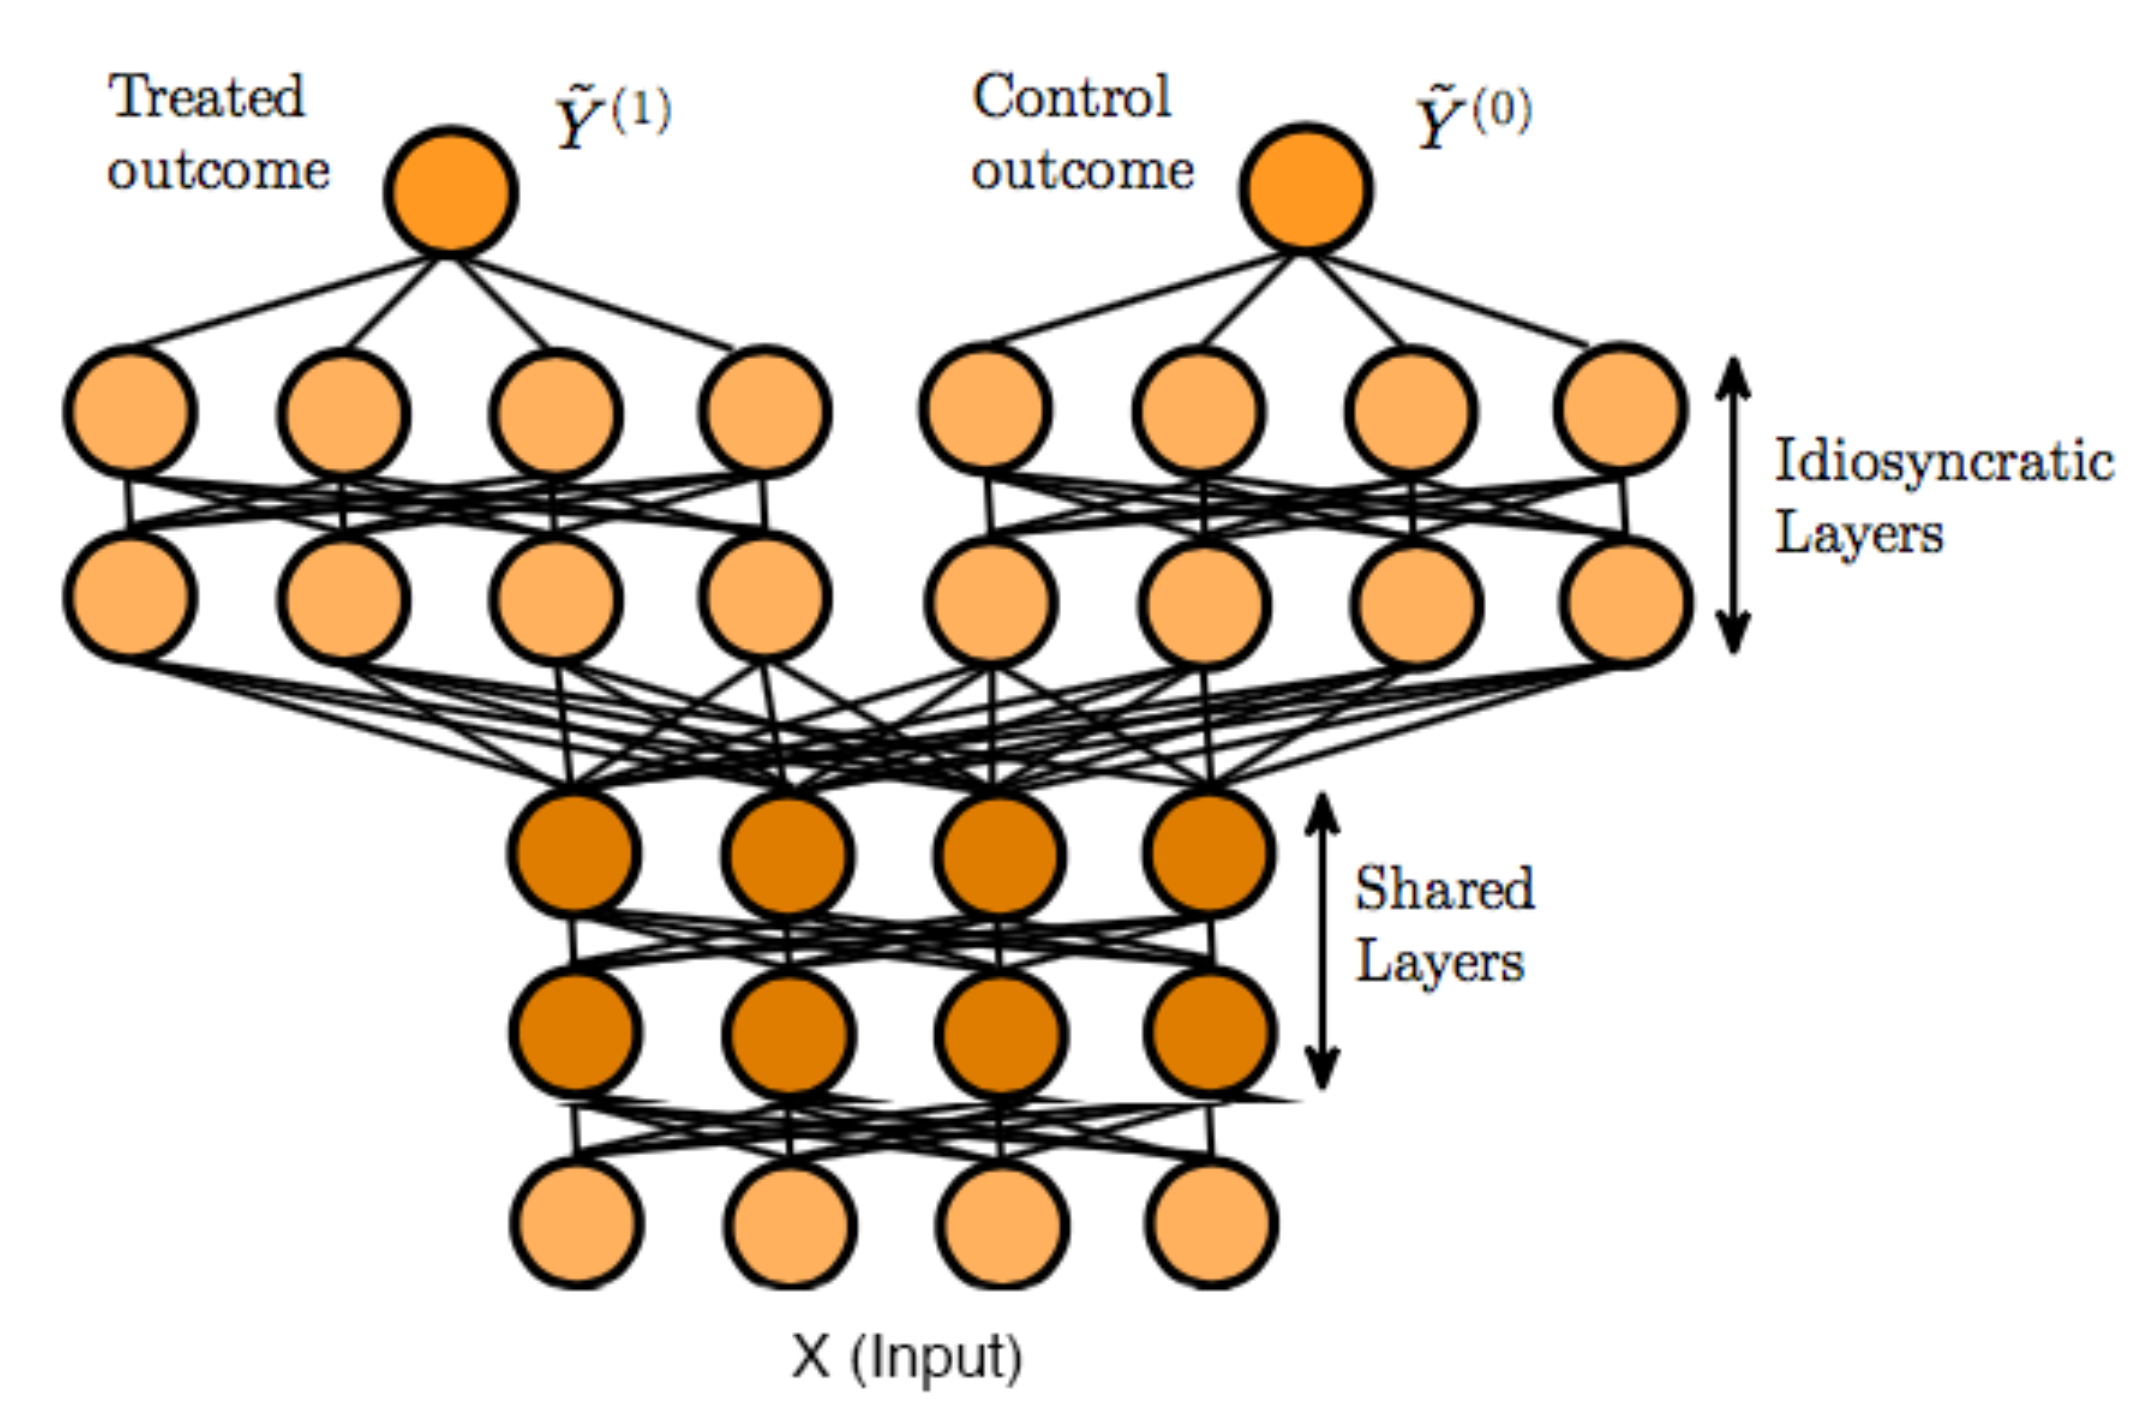
\includegraphics[width=0.8\textwidth]{figures/chapter-4/architecture-learning-motivation.png}
	\caption{Architecture Learning}\label{fig:architecture-learning-motivation}
\end{figure}

In this chapter we propose an efficient approach for automatically learning appropriate architectures of deep neural networks for the task of counterfactual inference over observational data by exploiting inferred characteristics of the dataset. For instance, if one of the outcomes in the data is estimated to follow a more complex function than the other, this should be reflected in a potentially asymmetric architecture which utilises a greater number of outcome-specific layers for the more complex outcome.


%The approach does not rely on expensive hyper-parameter search and is achieved by exploiting inferred characteristics of the dataset such as the propensity score, the similarity between the different outcome surfaces and the individual outcome-based complexity. 


\section{Architecture Learning}
Our model is able to automatically learn a suitable architecture for the DCN by exploiting relevant characteristics of the dataset which are specific to the problem of causal inference. These characteristics such as the \emph{selection bias}, the \emph{shared complexity} of the response surfaces, and the \emph{individual complexity} of each outcome function, can be inferred from the data to inspire a suitable architecture. This way, we achieve an efficient method of model-selection while avoiding computationally expensive hyper-parameter optimisations over the search space of possible architectures. 

The approach is based on the observation that certain architectures are more suitable than others for the task of counterfactual inference. Concretely, it can be shown empirically using traditional hyper-parameter optimisation that the best-performing architectures consistently follow specific \emph{ empiric ratios} between the number of shared and total layers, and the number of respective outcome-specific and total layers.

The optimal ratios are not static, however, but depend on specific characteristics of the dataset. Once these characteristics are known, we can use our empirical model to automatically infer the desired number of layers. This way, we obtain a suitable DCN architecture without the need to perform a hyper-parameter search.

In the following, we will discuss each characteristic in detail, including its intuition and formalisation. We present how the characteristic can be inferred from the data and how they might inform the architecture of the DCN.


\subsection{Relevant Characteristics} \label{sec:relevant-characteristics}
For the problem of counterfactual inference, we have identified the following main characteristics of the data. 

\subsubsection{(a) Selection Bias}
Each dataset can be considered a partition  of subjects into treated and untreated (control) subjects depending on their treatment assignment indicator $W_i$. Governed by the underlying treatment policy the dataset might be heavily imbalanced and skewed towards a specific treatment. 
Intuitively, this potential imbalance is relevant for our model because we might profit from a corresponding asymmetric architecture, i.e. a model where the number of outcome-specific layers differ from each other. 

Formally, the selection bias $\mathbf{B}$ can be quantified in terms of the average propensity score 
$$
\mathbf{B} = \frac{1}{n} \cdot \sum \limits_{{i=0}}^{n-1}  \mathbb{P}(W_i = 1 \mid X_i).
$$

The individual propensity scores can be estimated from the dataset using a neural network for which we treat the prediction of the treatment assignment as a binary classification problem in supervised learning. 



\subsubsection{(b) Similarity of  Outcome Response Surfaces}
The different outcome functions of the treated and untreated subjects can be conceptualised in terms of a shared part governed by features and their correlations that are mostly the same for both outcomes and an outcome-specific part that is inherently different. 

Intuitively, if the outcome functions are potentially complex but rather similar to each other, this should be reflected in a high number of shared layers in the network in contrast to a relatively low number of outcome-specific layers. 

Formally, we can model the different outcomes as functions
\begin{align}
\label{eqn:outcome-functions}
\begin{split}
f_1(X_i) =  \underbrace{g(X_i, \lambda^{(1)})}_{\text{shared}} +   \beta_1 \cdot \underbrace{ exp(h_1(X_i, \mu^{(1)}))}_{\text{outcome-specific}}
\\
f_0(X_i) = \overbrace{g(X_i, \lambda^{(0)})} +  \beta_0 \cdot \underbrace{exp(h_0(X_i, \mu^{(0)}))}_{\text{outcome-specific}}
\end{split}
\end{align}


where $g$ represents a common function and $h_0, h_1$ are outcome-specific (e.g. polynomial functions of different degrees). The relative weight of the common part in comparison to the outcome-specific part is captured by $\beta_0, \beta_1 \in \mathbb{R}$ (see below). In this model, the vectors $\lambda^{(1)}, \mu^{(1)}$ represent the coefficients of a specific response surface for the factual outcome whereas we model their counterfactual counterparts as
\begin{equation}
\label{eqn:mu_and_sigma}
\lambda^{(0)}_i \sim \mathcal{N}(\lambda^{(1)}_i, \sigma)  \hspace{1cm} \mu^{(0)}_i \sim \mathcal{N}(\mu^{(1)}_i, \sigma).
\end{equation}


This way, we can use the parameter $\sigma \in \mathbb{R}_{\geq0}$ to introduce a measure of similarity $\mathbf{S} \propto \sigma$ between the two outcome surfaces. A low sigma corresponds to a high similarity which should be reflected in a large amount of shared layers, whereas a large sigma should result in a smaller proportion of shared layers. 

There are multiple ways to estimate $\mathbf{S}$ for a new dataset. In our approach, we train two separate feed-forward neural networks -- one exclusively for the treated subjects and one exclusively for the untreated subjects. After training, we compare the coefficients according to equation $\ref{eqn:mu_and_sigma}$ to get an empirical estimate for $\mathbf{S}$. 
% CRITICAL This is not clear at all. How exactly do we 'compare' the coefficients? 
%TODO More precisely. What is the architecture of the networks? How do they relate to the metric above? How do we compare the coefficients. 

\subsubsection{(c) Individual Complexity of each Response Surface}
In addition to the complexity that is shared across both response surfaces, the outcomes typically possess an individual outcome-specific part that follows a completely different type of function. For instance, one of the outcomes might be linear whereas the other outcome might be a high-degree  polynomial function. 
Intuitively, the outcome with the more complex function should have a higher number of outcome-specific layers in our model in order to capture the more complex correlations between the features, leading to an overall asymmetric architecture. 

In order to formalise the outcome-specific complexity, we use the same model for the outcome functions as defined in equation \ref{eqn:outcome-functions}. This time we focus on the parameters $\beta_0, \beta_1 \in \mathbb{R}$ which can be used to model the relative weight that is put on the outcome-specific part in comparison to the shared part. A low value for $\beta_0$ or $\beta_1$ corresponds to a simpler individual response surface whereas higher values lead to more complex functions.  

This way, we achieve a measurement of the individual outcome-complexities $\mathbf{C_0} \propto \beta_0$ and $\mathbf{C_1} \propto \beta_1$.
% CRITICAL How do I learn this? 

\subsection{Empirical Model} \label{sec:empirical-model}
Our heuristic approach is based on the observation that --- depending on the characteristics defined above --- the best-performing architectures consistently express certain empirical ratios for the different numbers of layers. This way, we can create a model $\mathcal{F}$ with 

\begin{equation}
\mathcal{F}(\mathbf{B}, \mathbf{S}, \mathbf{C_0}, \mathbf{C_1}) = \tilde{\mathbf{R}} = \begin{bmatrix}
\tilde{R_{s}} \\
\tilde{R_{i,0}} \\
\tilde{R_{i,1}}
\end{bmatrix} 
\end{equation}

that takes as input the different characteristics and outputs a vector $\tilde{\mathbf{R}}$ that contains the estimated appropriate ratios 

\begin{align} 
\tilde{R_{s}} = \frac{L_{s}}{L_{\text{total}}} && \tilde{R_{i,0}} = \frac{R_{i,0}}{L_{\text{total}}} && \tilde{R_{i,1}} =\frac{R_{i,1}}{L_{\text{total}}}
\end{align} 
between the respective layers and the total number of layers $L_{\text{total}}$. 

We train the model using  synthetically-generated datasets (see section \ref{sec:data-generation}) for which we have full control over the different characteristics and use hyper-parameter optimisation such as grid-search over the set of different distributions of a fixed amount of layers to find the best-performing ratios. These ratios are then used as our target label in a supervised learning setting to train our empirical model $\mathcal{F}$. 


\subsection{Architecture Learning Algorithm}
Having defined and formalised the relevant characteristics of the dataset we can derive a suitable DCN architecture for a new dataset using the empirical model as outlined in algorithm \ref{fig:algorithm}. 

First, we estimate the characteristics $\mathbf{B}$, $\mathbf{S}$, $\mathbf{C_0}, \mathbf{C_1}$ of the dataset, as described in section  \ref{sec:relevant-characteristics} (i.e. by training separate neural networks to estimate the average propensity score and the respective shared and individual complexity measures of the two response surfaces). 

The estimated characteristics $\tilde{\mathbf{B}}$, $\tilde{\mathbf{S}}$, $\tilde{\mathbf{C_0}}, \tilde{\mathbf{C_1}}$ are then used as input features for our empirical model $\mathcal{F}$. Since we cannot be sure that the ratios provided by $\mathcal{F}$ have the property $\tilde{R_{s}} + \tilde{R_{i,0}} + \tilde{R_{i,1}} = 1 $, we are running a \emph{softmax function} $\sigma$ defined as  

\begin{equation}
\sigma(\mathbf{x})_i = \frac{e^{\mathbf{x}_i}}{\sum_{k=1}^{K}e^{\mathbf{x}_k}}
\end{equation}

where $\mathbf{x}$ is a $K$-dimensional vector and $i = 1, 2, \dots, K$ on the output vector $\tilde{\mathbf{R}}$ to normalise the estimated ratios making sure they add up to $1$. 
%We will refer to the \emph{deep counterfactual network} whose architecture we learned using our approach as \emph{DCN-LA}. It is trained  analogously to a traditional DCN as described in section \ref{sec:dcn-training}. 


% GRAPH Update the algorithm accordingly to reflect empirial model and vector R
\begin{algorithm}
	\caption{Architecture Learning}\label{fig:algorithm}
	\begin{algorithmic}[1]
		
		\Procedure{Architecture Learning for DCN}{} \\
		\textbf{Input:} Dataset $\mathcal{D}$, $L_{\text{total}}$  
		\State \emph{\# Learn Characteristics from dataset}
		\State $\ \tilde{\mathbf{B}} \gets \textit{estimate selection bias (a)}$
		\State $\ \tilde{\mathbf{S}} \gets \textit{estimate response surface similarity (b)}$
		\State $\ \tilde{\mathbf{C_0}}, \tilde{\mathbf{C_1}} \gets \textit{estimate individual complexity (c)}$\\
		\State \emph{\# Derive Architecture}
		\State $\ {L_s} \gets \tilde{L_s}(\tilde{\mathbf{B}}, \tilde{\mathbf{S}}, \tilde{\mathbf{C_0}}, L_{\text{total}})$
		\State $\ {L_{i,0}}\gets \tilde{L_{i,0}}(\tilde{\mathbf{B}}, \tilde{\mathbf{S}}, \tilde{\mathbf{C_0}}, L_{\text{total}})$
		\State $\ {L_{i,1}}\gets \tilde{L_{i,1}}(\tilde{\mathbf{B}}, \tilde{\mathbf{S}}, \tilde{\mathbf{C_1}}, L_{\text{total}})$ \\
		\textbf{Return:} $L_s, L_{i,0}, L_{i,1}$ 
		
		\EndProcedure
	\end{algorithmic}
\end{algorithm}


Concluding, it can be said that by using our approach we can profit from the best-performing ratios of the pre-trained empirical model, allowing us to directly estimate an appropriate architecture for any new dataset $\mathcal{D}$ without the need for computationally expensive hyper-parameter optimisation.  
	

\part{Experiments and Results}
%\begin{savequote}[8cm]
%\textlatin{Jedem Anfang wohnt ein Zauber innne.}
%
%In the core of every beginning lives magic.
%  \qauthor{--- Hermann Hesse's \textit{Stufen}}
%\end{savequote}

\chapter{\label{ch:5-experiments}Experiments} 

%\minitoc

\section{Deep Counterfactual Networks}
In chapter \ref{ch:3-DCNs} we introduced \emph{deep counterfactual networks} (DCN) with a propensity-based dropout scheme (PD) for the task of counterfactual inference. In the following, we will run a number of experiments on the model to evaluate its performance and compare it to a variety of baseline methods and existing competing approaches. 

Firstly, we introduce the dataset that we are running the experiments on before describing the experimental setup in detail including the used hyper-parameters and relevant implementation details. Finally, we show the results of the experiments provide a discussion of the outcomes and its implications.  

\subsection{Dataset}
As described in section \ref{sec:counterfactual-inference}, due to the very nature of counterfactual inference we are never able to access the ground truth for the counterfactual outcomes for any observational dataset. This poses an enormous challenge when it comes to evaluating the performance of any model used for causal inference on real-world data. In order to deal with this issue, we follow (Hill) % CITE Hill, Johansson..
and adopt a \emph{semi-synthetic} experimental setup for which we use the actual covariates and treatment assignments from the dataset but simulate the outcomes in order to have access to both the factual and the counterfactual outcomes. Nonetheless, it is important to note that the counterfactual outcome is only used for evaluation purposes and considered as unavailable during training time. 

The experiments are conducted on the Infant Health and Development Program (IHDP) dataset that was introduced in (Hill, 2012). % CITE Hill
 program that was carried out in the second half of the 1980s tried to aid premature infants at an early age to enhance their cognitive abilities measured in terms of the IQ score. The dataset consists of a total of 747 subjects out of which 139 were treated and 608 controlled. Each subject has 6 continuous and 19 binary features representing attributes of the child such as birth weight, sex, and weeks born pre-term, and relevant attributes of the mother measured around the time of giving birth (e.g. age, educational status, etc.). The outcome are simulated based on a functions that are described as "Response Surface B" setting in (Hill, 2012). % CITE HILL 2012
 

\subsection{Experiment Setup} \label{sec:pbd-experiment-setup}
We are evaluating the performance of a \emph{deep counterfactual network} with \emph{propensity-dropout} which we will refer to as DCN-PD. In our experiment we are using an architecture with $L_s = 2, L_{i,0} =2 , L_{i,1} = 2$, thus $L_{\text{total}} = 4$ total layers, % IMPORTANT Do we consider the depth or the sum of layes as total? Shouldn't it be 6 instead?
and utilise a fixed number of $h_s^{(l)} = h_{i,0}^{(l)} = h_{i,1}^{(l)} = 200$ hidden units for the $l^{th}$ layer in the network. We are using a ReLU activation function for our network and we evaluate the performance of the model in terms of the mean squared error (MSE)
% EQUATION Make sure this is correct!
\begin{equation} \label{eq:mse-ite}
\text{MSE} = \frac{1}{n}\sum_{i=1}^{n} (T_i(x) - \tilde{T}_i(x))^2 = \frac{1}{n}\sum_{i=1}^{n} ((Y_i^{(1)} - Y_i^{(0)}) - (\tilde{Y}_i^{(1)} - \tilde{Y}_i^{(0)}))^2
\end{equation}
 of the estimated treatment effect and the true treatment effect (as defined in equation \ref{eq:ite}).  

The IHDP dataset is split into a training set comprising 80\% of the data and a test set with the remaining 20\%. We run a total of $N_E = 100$ experiments, each time drawing new outcomes according to the data generation model described in (Hill, 2012), % CITE Hill
and report the average MSE across all experiments, each time evaluated exclusively on the out-of-sample test set. 

For the \emph{propensity network} (see \ref{sec:multi-task-learning}) that is used to estimate the propensity scores for each subject, we used $L_p = 2$ layers with $h_p^{(l)}) = 25$ hidden units per layer, trained using an Adam optimiser % CITE ADAM 
and Xavier initialisation. % CITE XAVIER
The propensity-dropout is applied as described in section \ref{sec:propensity-based-dropout} and uses $\lambda = 1$. 

% TODO Should I mention Tensorflow? 
%The neural network is implemented in Tensorflow %CITE TEnsorflow
\subsection{Results and Discussion}
Firstly, we investigate the impact of our propensity-dropout scheme by comparing a DCN-PD to other deep counterfactual networks with regular dropout schemes (that is the dropout probability is fixed throughout all samples and for the hidden units in all layers). Figure \ref{fig:propensity-dropout-boxplot} shows the marginal gains in terms of the MSE achieved by the DCN-PD (right) over a DCN with a dropout probability $p=0.2$ (middle), and a DCN with dropout probability $p=0.5$ (left) in form of a box plot. 



%As we can see in Fig. 3, the DCN- PD model offers a significant improvement over the two DCN models for which the dropout probabilities are uni- form over all the training examples. This result implies that the DCN-PD model generalizes better to the true fea-
%Figure 3. Performance gain achieved by propensity-dropout.
%ture distribution when trained with a biased dataset as com- pared to DCN with regular dropout, which suggests that propensity-dropout is a good regularizer for causal infer- ence.


\begin{figure}[h]
	\centering
	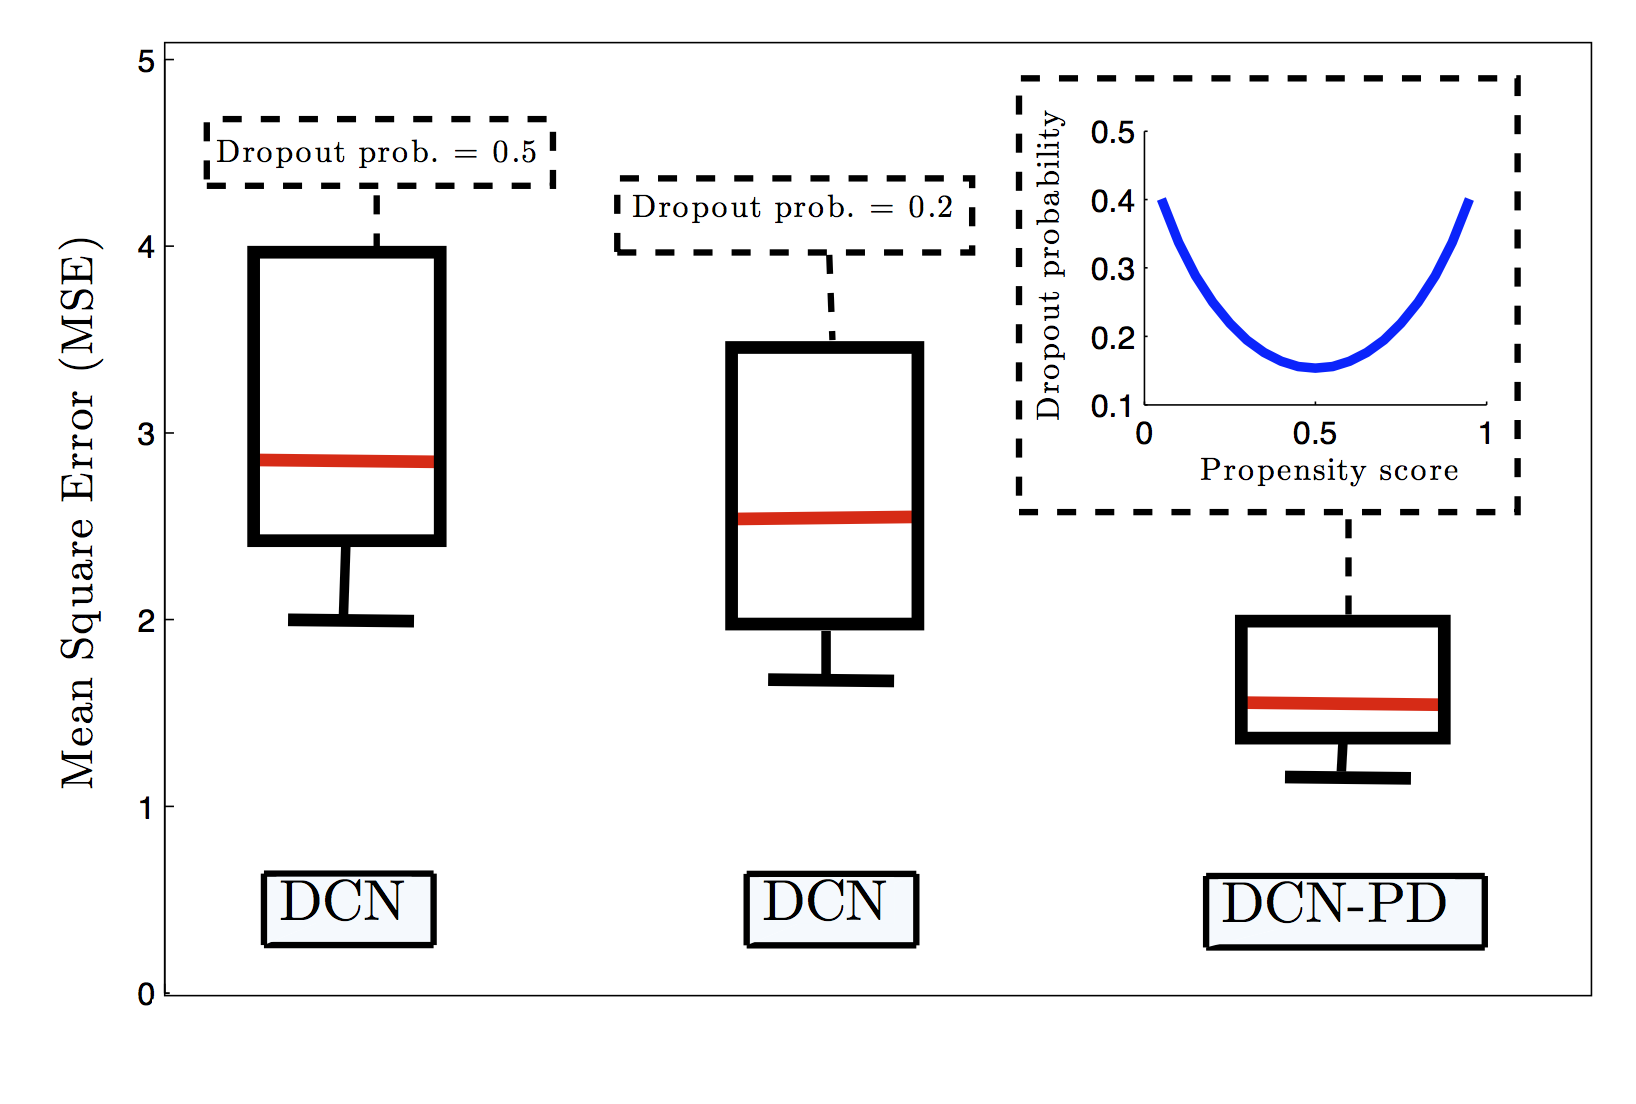
\includegraphics[width=0.9\textwidth]{figures/chapter-5/pd-boxplot.png}
	\caption{Comparison between the performance of a DCN with propensity-based dropout (right) and DCNs with regular dropout schemes (middle, left) in terms of the mean squared error (lower is better). The propensity-dropout has a regularising effect towards the selection bias and provides the model a higher degree of generalisation. }\label{fig:propensity-dropout-boxplot}
\end{figure}

As we can observe in the figure, our propensity-based dropout scheme provides a significant improvement over the alternative DCNs for which the  dropout probabilities are uniform throughout all samples in the training set. The result implies that the propensity-based dropout helps the DCN to generalise better to the true feature distribution when trained with an biased dataset such as IHDP (139 treated vs. 608 controlled subjects). Consequently, this suggest that propensity-dropout can be an effective regulariser for the task of counterfactual inference. 

In the following, we will look at the performance of a DCN and DCN-PD in comparison to competing state-of-the-art methods shown in table \ref{tab:dcn-pd-results}. Concretely, we compare the mean MSE (aggregated over $N_E = 100$ experiments) that is achieved by our models to the MSE of k-Nearest-Neighbour matching (k-NN), Causal Forests with double-sample tree (WagerAthey, 2015), % CITE Wager Athey
a classical feed-forward neural network with the treatment assignemnt as input feature (NN-4),
Bayesian Additive Regression Trees (BART) (Chipman) % CITE CHipman, Hill
and balancing neural networks (BNN) (Johanson) % CITE JOhannson
that we discussed in detail in section \ref{sec:representation-learning} and which represent the state-of-the-art for counterfactual inference. 
In order to ensure a fair comparison, for the BNN and the NN-4 we are also using $4$ layers, each with $200$ hidden units trying to hold as many hyper-parameters as possible constant. The DCN uses regular dropout scheme with a dropout probability of $p=0.2$ and the DCN-PD is regularised using our propensity-based dropout.

As we can see in table \ref{tab:dcn-pd-results}, the DCN-PD achieves the lowest MSE and outperforms the other methods. The BNN, representing  a strong benchmark as it effectively handles the selection bias by learning a balanced representation for the input features, represents the most competitive alternative. Lastly, the performance gains that our DCN-PD achieves over a the NN-4 model suggest that the multi-task learning framework is an effective conception of counterfactual inference that outperforms direct modelling approaches which consider the treatment assignment as a regular input feature.   %TODO Should I mention that DCNs don't perform too wel? 

Concluding, it can be said that our proposed model of deep counterfactual networks using propensity-dropout (DCN-PDs) represents a promising approach to using deep neural networks for counterfactual inference that it is able to compete with and potentially even outperform existing methods. 

% TODO Mention criticm ? 

\begin{table}[]
	\centering
	\begin{tabular}{@{}cc@{}}
		\toprule
		\textbf{Algorithm} & \textbf{MSE}                \\ \midrule
		k-NN               &   $5.30 \pm 0.30$           \\
		Causal Forest      &   $3.86 \pm 0.20$           \\
		BART               &   $3.50 \pm 0.20$           \\ 
		BNN                &   $2.45 \pm 0.10$           \\
		NN-4                &  $2.88 \pm 0.10$           \\
		DCN                &   $2.58 \pm 0.06$           \\
		DCN-PD             &   $2.05 \pm 0.03$          \\\bottomrule
	\end{tabular}
	\caption{Performance of Deep Counterfactual Networks (DCN) and Deep Counterfactual Networks with Propensity-Dropout (DCN-DP) in comparison with baseline methods and existing competing approaches}\label{tab:dcn-pd-results}
\end{table}


\section{Architecture Learning for DCN}
In chapter \ref{ch:4-DCN-LAs} we introduced an efficient approach to automatically infer an appropriate architecture for \emph{deep counterfactual networks} (DCN) without the need for computationally expensive hyper-parameter optimisation (e.g. grid search, random search, or bayesian optimisation). 

In the following, we will run a number of experiments to investigate the performance of the model with the inferred architecture. In particular, we investigate how the different characteristics (selection bias, shared complexity, and outcome-specific complexity) that we defined in section \ref{sec:relevant-characteristics} influence the learnt architecture and the performance of the model. 

Firstly, we introduce a purely synthetic dataset that gives us full control over the relevant characteristics, and a real-world dataset for which the characteristics have to be inferred according to our approach. Thereafter, we describe the experimental setup in detail including the used hyper-parameters and relevant implementation details before showing the results of the experiments and concluding with a discussion of the outcomes and its implications.  


\subsection{Datasets}
\subsubsection{Synthetic Model} \label{sec:synthetic-model}
For the synthetic model, we draw $n = 1000$ samples in the form of a tuple $\langle X_i, W_i, Y_i \rangle$ for each subject $i$. Each $X_i = (x_{i,0}, x_{i,1}, \ldots, x_{i,24})$ consists of $d = 25$ covariates for each subject which are independently drawn from a uniform distribution, i.e.  

\begin{equation}
x_{i,0}, x_{i,1}, \ldots, x_{i,24} \overset{iid}{\sim} \mathcal{U}(0, 1)
\end{equation}
keeping each covariate strictly non-negative. For the treatment assignment indicator $W_i \in \{0,1\}$, we define

\begin{equation}
\tilde{p}(X_i) =  \frac{1}{1 + exp(- \alpha\sum \limits_{{x_{j} \in X_i}} x_j)} % \mathbb{P}(W_i = 1 \mid X_i = x) =
\end{equation}
\begin{equation}
W_i \sim Bernoulli(\tilde{p}(X_i))
\end{equation}
where $\tilde{p}(X_i)$ represents the subject's propensity score and the parameter $\alpha \in \mathbb{R}_{\geq0}$ gives us a way to control the imbalance between the treated and untreated subjects. For $\alpha = 0$, we get $\tilde{p}(X_i) = 0.5$ corresponding to a maximum balance between the number of treated and untreated subjects whereas an increasing alpha shifts the distribution towards a higher proportion of treated subjects.
% TOTO Which quantity does it correspond to
We compute both outcomes $Y^{(0)}, Y^{(1)} \in \mathbb{R}$ as
\begin{equation}
Y^{(0)}_i = f_0(X_i) + \mathcal{N}(0, 1)
\end{equation}
\begin{equation}
Y^{(1)}_i = f_1(X_i) + \mathcal{N}(0, 1)
\end{equation}
which are governed by their corresponding outcome functions $f_0$ and $f_1$ defined as


\begin{equation}
f_1(X_i) = \sum \limits_{{x_{j} \in X_i}} \lambda^{(1)}_j x_j +  \beta^{(1)} \cdot exp(\sum \limits_{{x_{j} \in X_i}} \mu^{(1)}_j x_j^2)
\end{equation}

\begin{equation}
f_0(X_i) = \sum \limits_{{x_{j} \in X_i}} \lambda^{(0)}_j x_j +  \beta^{(0)} \cdot exp(\sum \limits_{{x_{j} \in X_i}} \mu^{(0)}_j x_j).
\end{equation}

Each outcome function consists of a linear part governed by the coefficients in the vectors $\lambda^{(0)}$ and $\lambda^{(1)}$ respectively, and an outcome-specific polynomial part inside the exponential function governed by the coefficients in the vectors $\mu^{(0)}$ and $\mu^{(1)}$. In the case of $f_1$ this is a quadratic function whereas for $f_0$ we are using a linear function. The parameters $\beta^{(0)}, \beta^{(1)} \in \mathbb{R}^0$ let us control the weight of the outcome-specific polynomial part in comparison to the common linear part. \\
% TODO Add A, B annotation for the different parts in the equation
% TODO Continue here. In the worst case, don't spend too much time thinking about the meaning. Come back to this later but for now just write the formula for drawing lambda and kappa. 

The vectors $\lambda^{(1)}, \mu^{(1)}$ for the treated outcome function $f_1$ are drawn based on the data generation process designated as the "Response Surface B" setting in (Hill, 2012). For the outcome function $f_0$ of untreated subjects, we draw the vectors $\lambda^{(0)}, \mu^{(0)}$ from a normal distribution centred around their corresponding treated counterpart, i.e.    
%TODO Cite Hill


\begin{equation}
\lambda^{(0)}_i \sim \mathcal{N}(\lambda^{(1)}_i, \sigma)  \hspace{1cm} \mu^{(0)}_i \sim \mathcal{N}(\mu^{(1)}_i, \sigma),
\end{equation}
with a standard deviation $\sigma$. This way, we can use the parameter $\sigma \in \mathbb{R}^0$ to control the similarity between the two outcome surfaces. 
Finally, we can set $Y_i = W_i \cdot Y^{(1)}_i + (1 - W_i) \cdot Y^{(0)}_i$ representing our \emph{factual outcome} for subject $i$. The other (i.e. counterfactual) outcome is not used in the training set but needed later for evaluation purposes. \\

In summary, we receive a synthetic model which is parametrised by $\alpha$, $\beta^{(0)}$, $\beta^{(1)}$, and $\sigma$ each corresponding directly to a different characteristic we are interested in. The parameter $\alpha$ defines the skewness of the treatment assignment (i.e. the portion of treated vs. untreated subjects) and corresponds to $\mathbf{B}$,  $\beta^{(0)}$ and $\beta^{(1)}$ define the emphasis of the outcome-specific parts of the equation in relation to their common linear part and correlate with $\mathbf{C_0}, \mathbf{C_1}$, and $\sigma$ determines the overall similarity between the two outcome surfaces directly corresponding to $\mathbf{S}$. 

% TODO Mention the similarities between the synthetic model and the empirical model

% TODO Add UNOS
\subsubsection{UNOS}
Lorem ipsum dolor sit amet consectetur adipiscing elit, sagittis id ultrices neque iaculis. Posuere vitae turpis tristique viverra himenaeos commodo euismod maecenas, magnis est urna placerat purus dolor arcu class mauris, eros metus adipiscing convallis lobortis ullamcorper justo. Tellus sem fringilla tristique elementum aliquet diam ac vestibulum nullam, volutpat nam lacinia ullamcorper turpis etiam nulla parturient ornare, sed magna egestas lorem sapien sodales imperdiet libero. Ipsum augue hac fusce ac semper feugiat proin aptent duis, consequat at leo facilisis posuere suscipit himenaeos gravida. Tempus nostra non lacus vivamus nunc mattis, nascetur semper platea cursus est.

\subsection{Experiment Setup}
The experiments are conducted in a setting similar to the ones described in section \ref{sec:pbd-experiment-setup}. For instance, this means using ReLU activation functions, utilising 200 hidden units per layer, and considering the MSE over estimated treatment effect (see equation \ref{eq:mse-ite})as our evaluation metric. 

The main difference is that we are not assuming any specific values for the numbers of layers $L_s, L_{i,0},$ and $L_{i,1}$ as it is our very objective to automatically learn an appropriate architecture for our model by exploiting inferred characteristics of the dataset. For the sake of fairness and  comparability with the competing models, we limit the total number of layers in the network to $L_{\text{total}} = 4$. 

The synthetic and the UNOS dataset are each split into a training set comprising 80\% of the data and a test set with the remaining 20\%. We run a total of $N_E = 100$ experiments, each time drawing new outcomes according to the data generation models in the previous sections
and report the average MSE across all experiments, each time evaluated exclusively on the out-of-sample test set. 

%For the \emph{propensity network} (see \ref{sec:multi-task-learning}) that is used to estimate the propensity scores for each subject, we used $L_p = 2$ layers with $h_p^{(l)}) = 25$ hidden units per layer, trained using an Adam optimiser % CITE ADAM 
%and Xavier initialisation. % CITE XAVIER
%The propensity-dropout is applied as described in section \ref{sec:propensity-based-dropout} and uses $\lambda = 1$. 

\subsection{Results}

\subsubsection{Synthetic Model}
Normally, we would first need to estimate the relevant characteristics from the data (see algorithm \ref{fig:algorithm}) in order to use them to infer an appropriate architecture for the DCN-LA. For the synthetic dataset, however, we can skip the estimation as we have access to the parameters $\mathbf{B}, \mathbf{S}, \mathbf{C_0}, \mathbf{C_1}$ directly as a part of our generation process described in  section \ref{sec:synthetic-model}. 

In the following, we investigate how the inferred architecture of the DCN-LA is influenced by the characteristics of the synthetic dataset.  \\

\textbf{i) Influence of similarity measure S:} 
Figure \ref{fig:syn-sigma} shows the effect of the similarity measure \textbf{S} of a dataset on the DCN-LA in terms of the learnt architecture (\ref{fig:syn-sigma-ratios}) and its performance (\ref{fig:syn-sigma-mse}) in comparison with competing approaches. 

Looking at the architecture, we can see that for synthetic datasets with a high level of similarity ($\mathbf{S} \approx 0$), the DCN-LA learns an architecture with a high number of shared layers in relation to the total number of layers. In contrast, for datasets with a decreasing similarity ($\mathbf{S} \rightarrow 2$) % MATH Is this an appropriate notation? 
the number of shared layers drops in favour of more outcome-specific layers. 

Figure \ref{fig:syn-sigma-mse} shows the MSE of the individualised treatment effect (ITE) for our evaluation of the learnt architecture (DCN-LA) in comparison with other existing methods. As can be seen in the graph, unlike a standard feed-forward neural network (NN4), the DCN-LA is able to adapt well even in cases where the response surface are very different from each other. This is explained by the fact that the DCN-LA accommodates different response surfaces by learning an architecture with few numbers of shared layers and a high number of individual layers. \\
% GRAPHS Redo graphs. S instead of sigma. Make axis labels bigger. Re-label legend to reflect Rx etc...
\begin{figure}[h]
	\centering
		\caption{A caption for both images}\label{fig:syn-sigma}
	\begin{subfigure}{\linewidth}
		\centering
		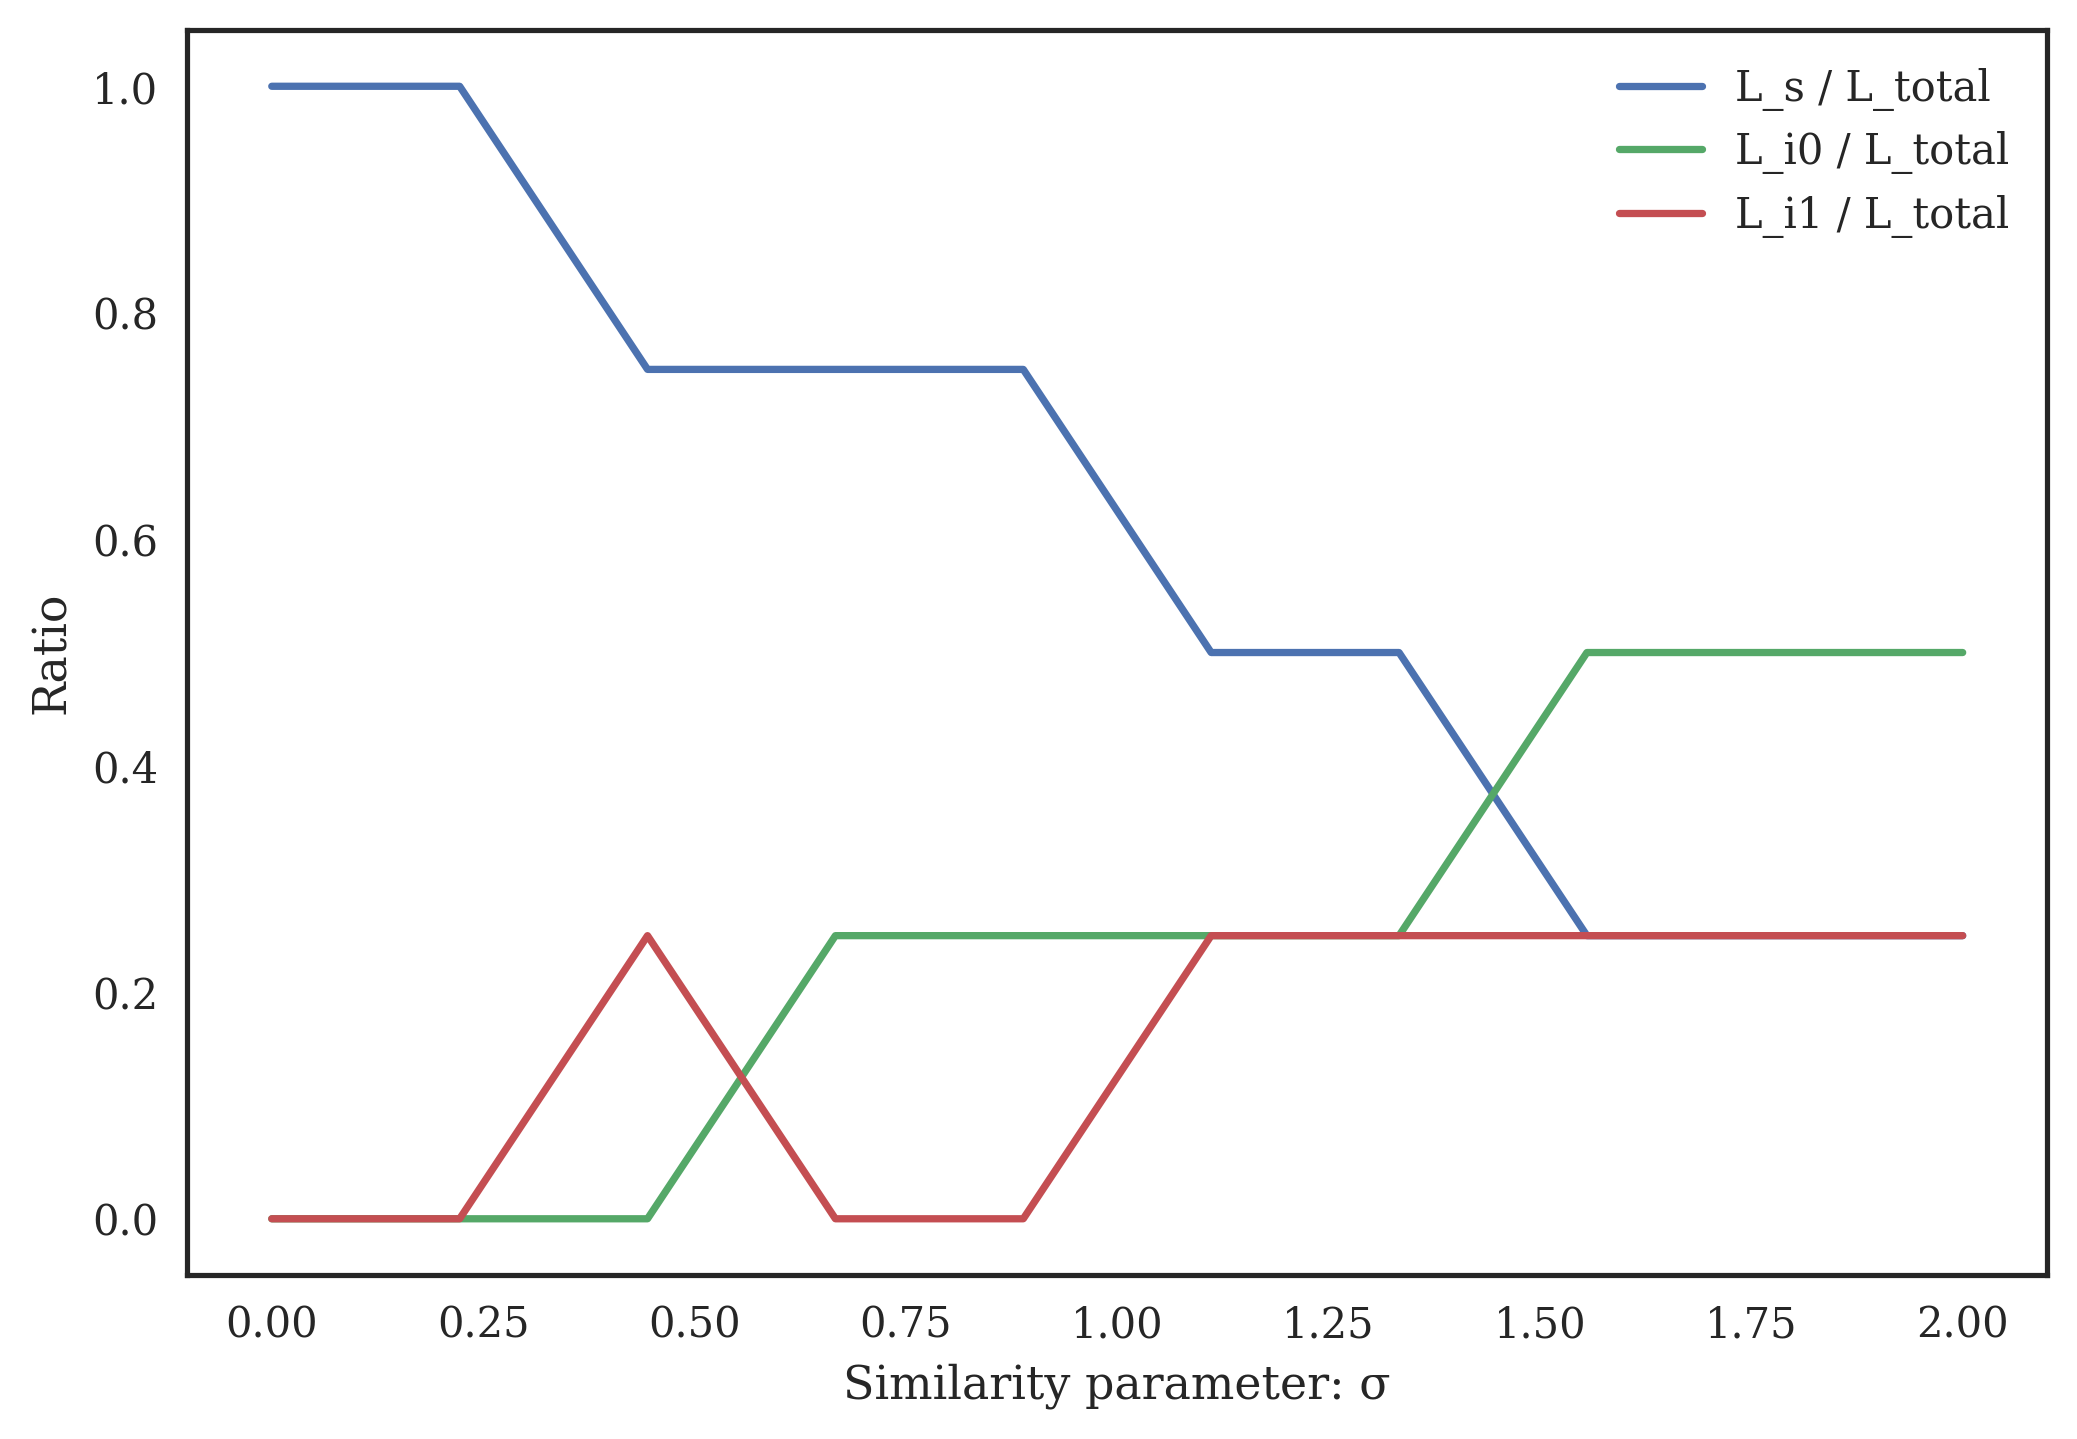
\includegraphics[width=.8\linewidth]{figures/chapter-5/syn-ratio-sigma.png}
		\caption{Learnt architecture (in terms of the ratios \textbf{R}) of the DCN-LA depending on the similarity parameter \textbf{S} of the input dataset. With decreasing similarity (higher sigma), the number of shared layers drops in favour of the outcome specific layers.}\label{fig:syn-sigma-ratios}
	\end{subfigure}
	\begin{subfigure}{\linewidth}
		\centering
		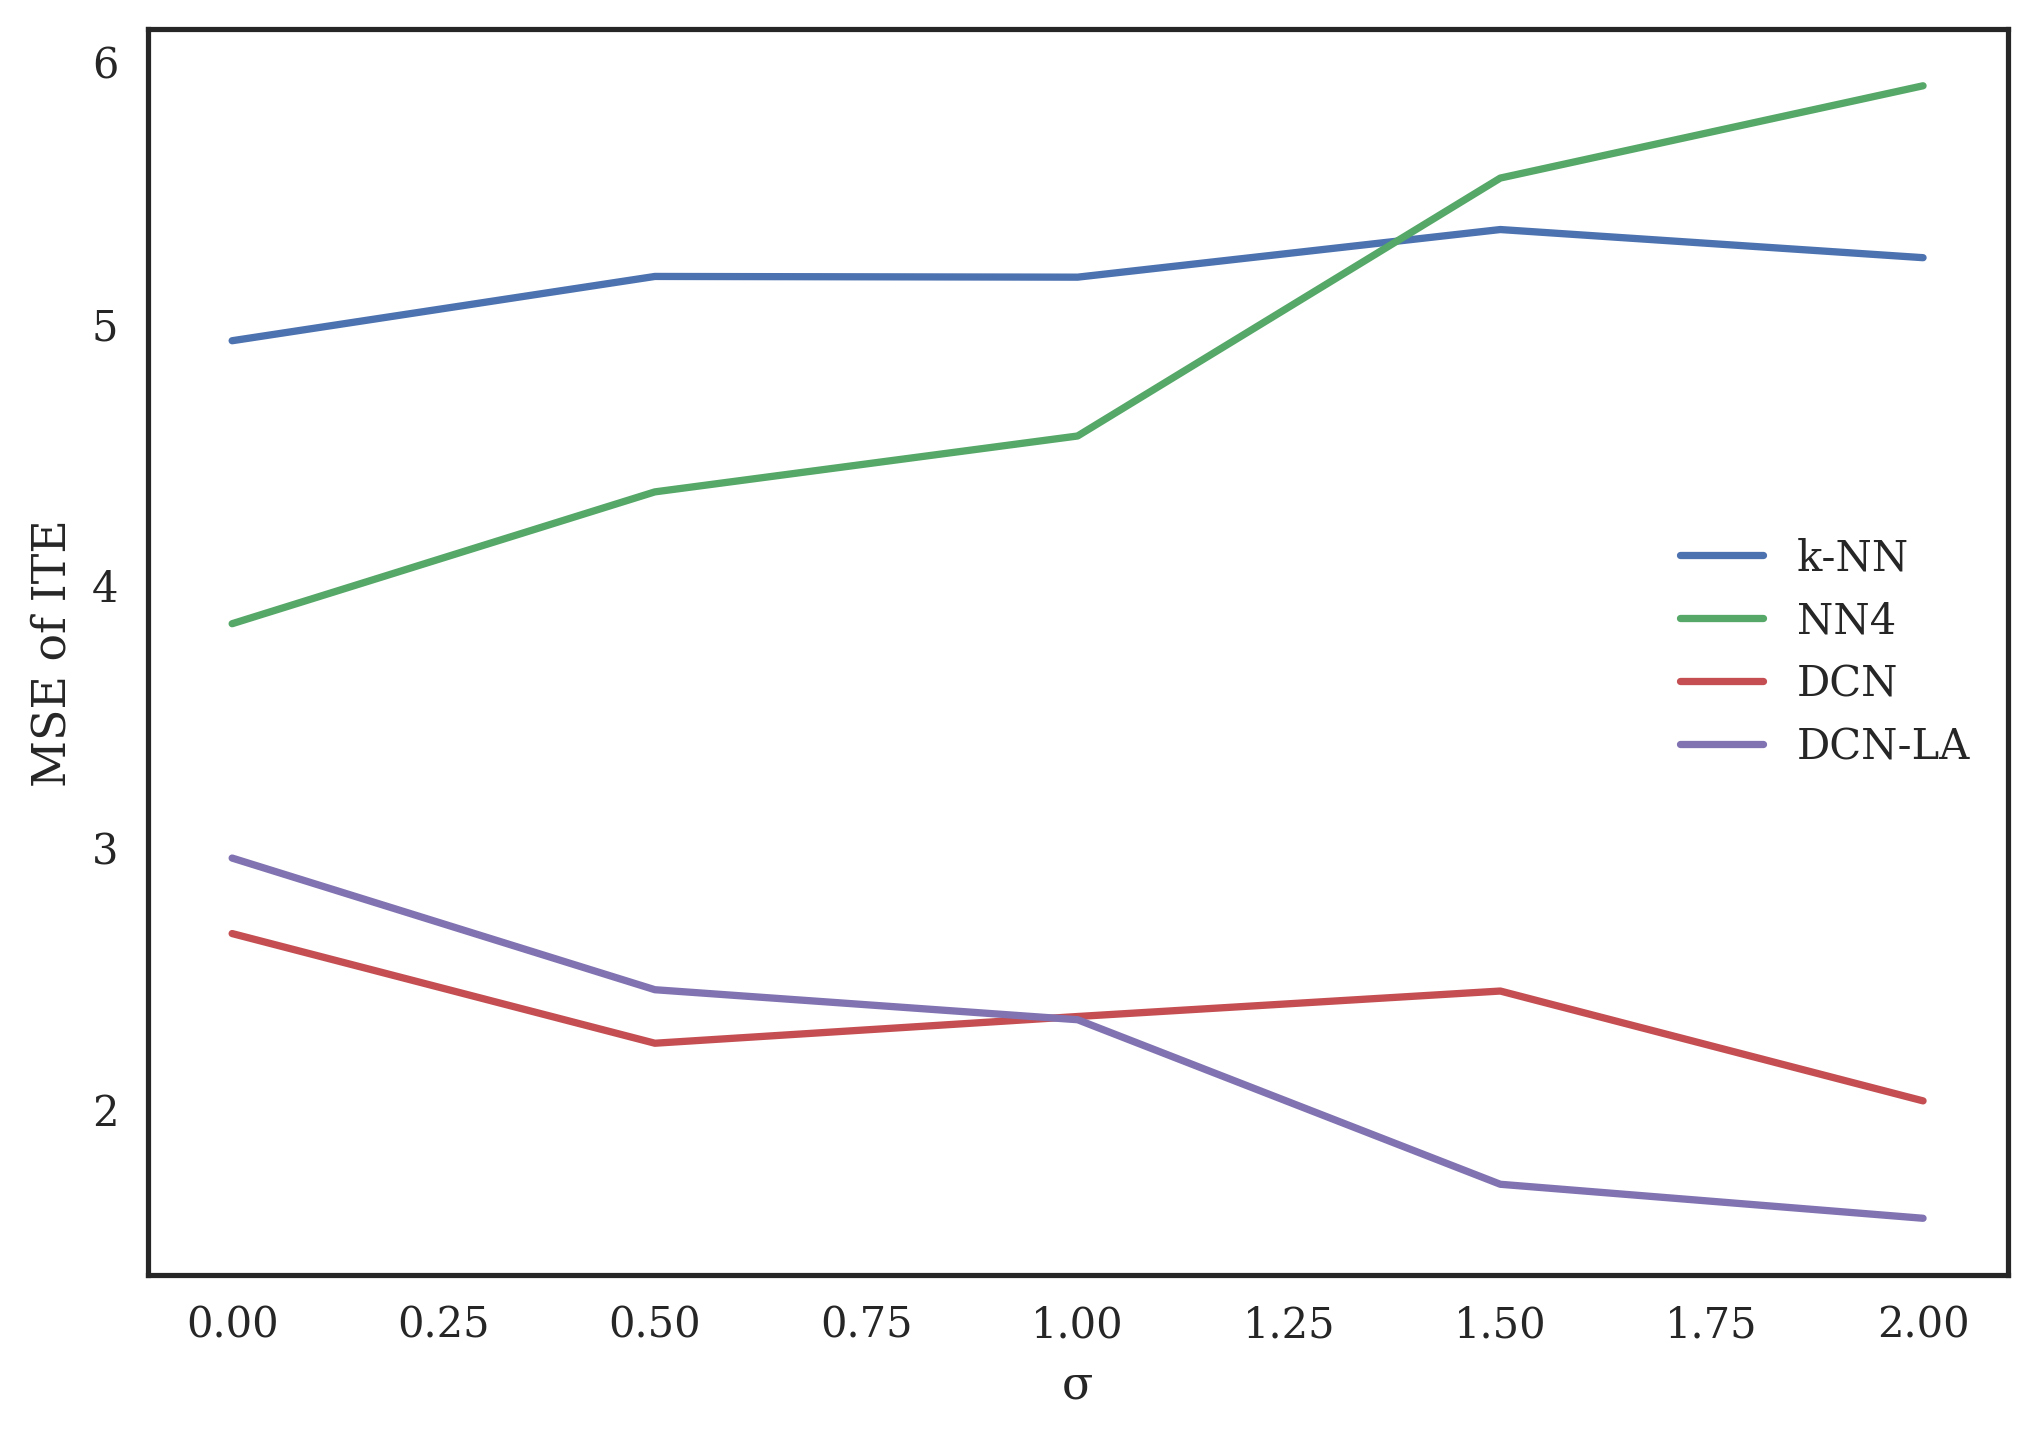
\includegraphics[width=.8\linewidth]{figures/chapter-5/syn-mse-sigma.png}
		\caption{Performances of DCN-LA, DCN, NN4, and k-NN for input datasets with different similarities. The DCN-LA is able to adapt well different response surfaces by utilising a higher number of outcome-specific layers. }\label{fig:syn-sigma-mse}
	\end{subfigure}  
 
\end{figure}  

\textbf{ii) Influence of the selection bias and response surface complexity:}
Figure \ref{fig:syn-beta} illustrates how the learnt architecture of the DCN-LA changes depending on the parameters $\mathbf{C}_0$ and $\mathbf{C}_1$ which measure the individual complexity of the respective outcome surface. As can be observed in the graph, the more complex the response surface of $Y^{(j)}$, the higher is the number of outcome-specific layers $L_{j,0}$ in the learnt model in relation to the shared layers and the outcome-specific layers of $Y^{(1-j)}$ leading to an asymmetric architecture. 

 \begin{figure}[h]
	\centering
	\caption[ The average and standard deviation of critical parameters ]
	{\small The average and standard deviation of critical parameters: Region R4} 
	\label{fig:syn-beta}
	\begin{subfigure}[b]{0.475\textwidth}
		\centering
		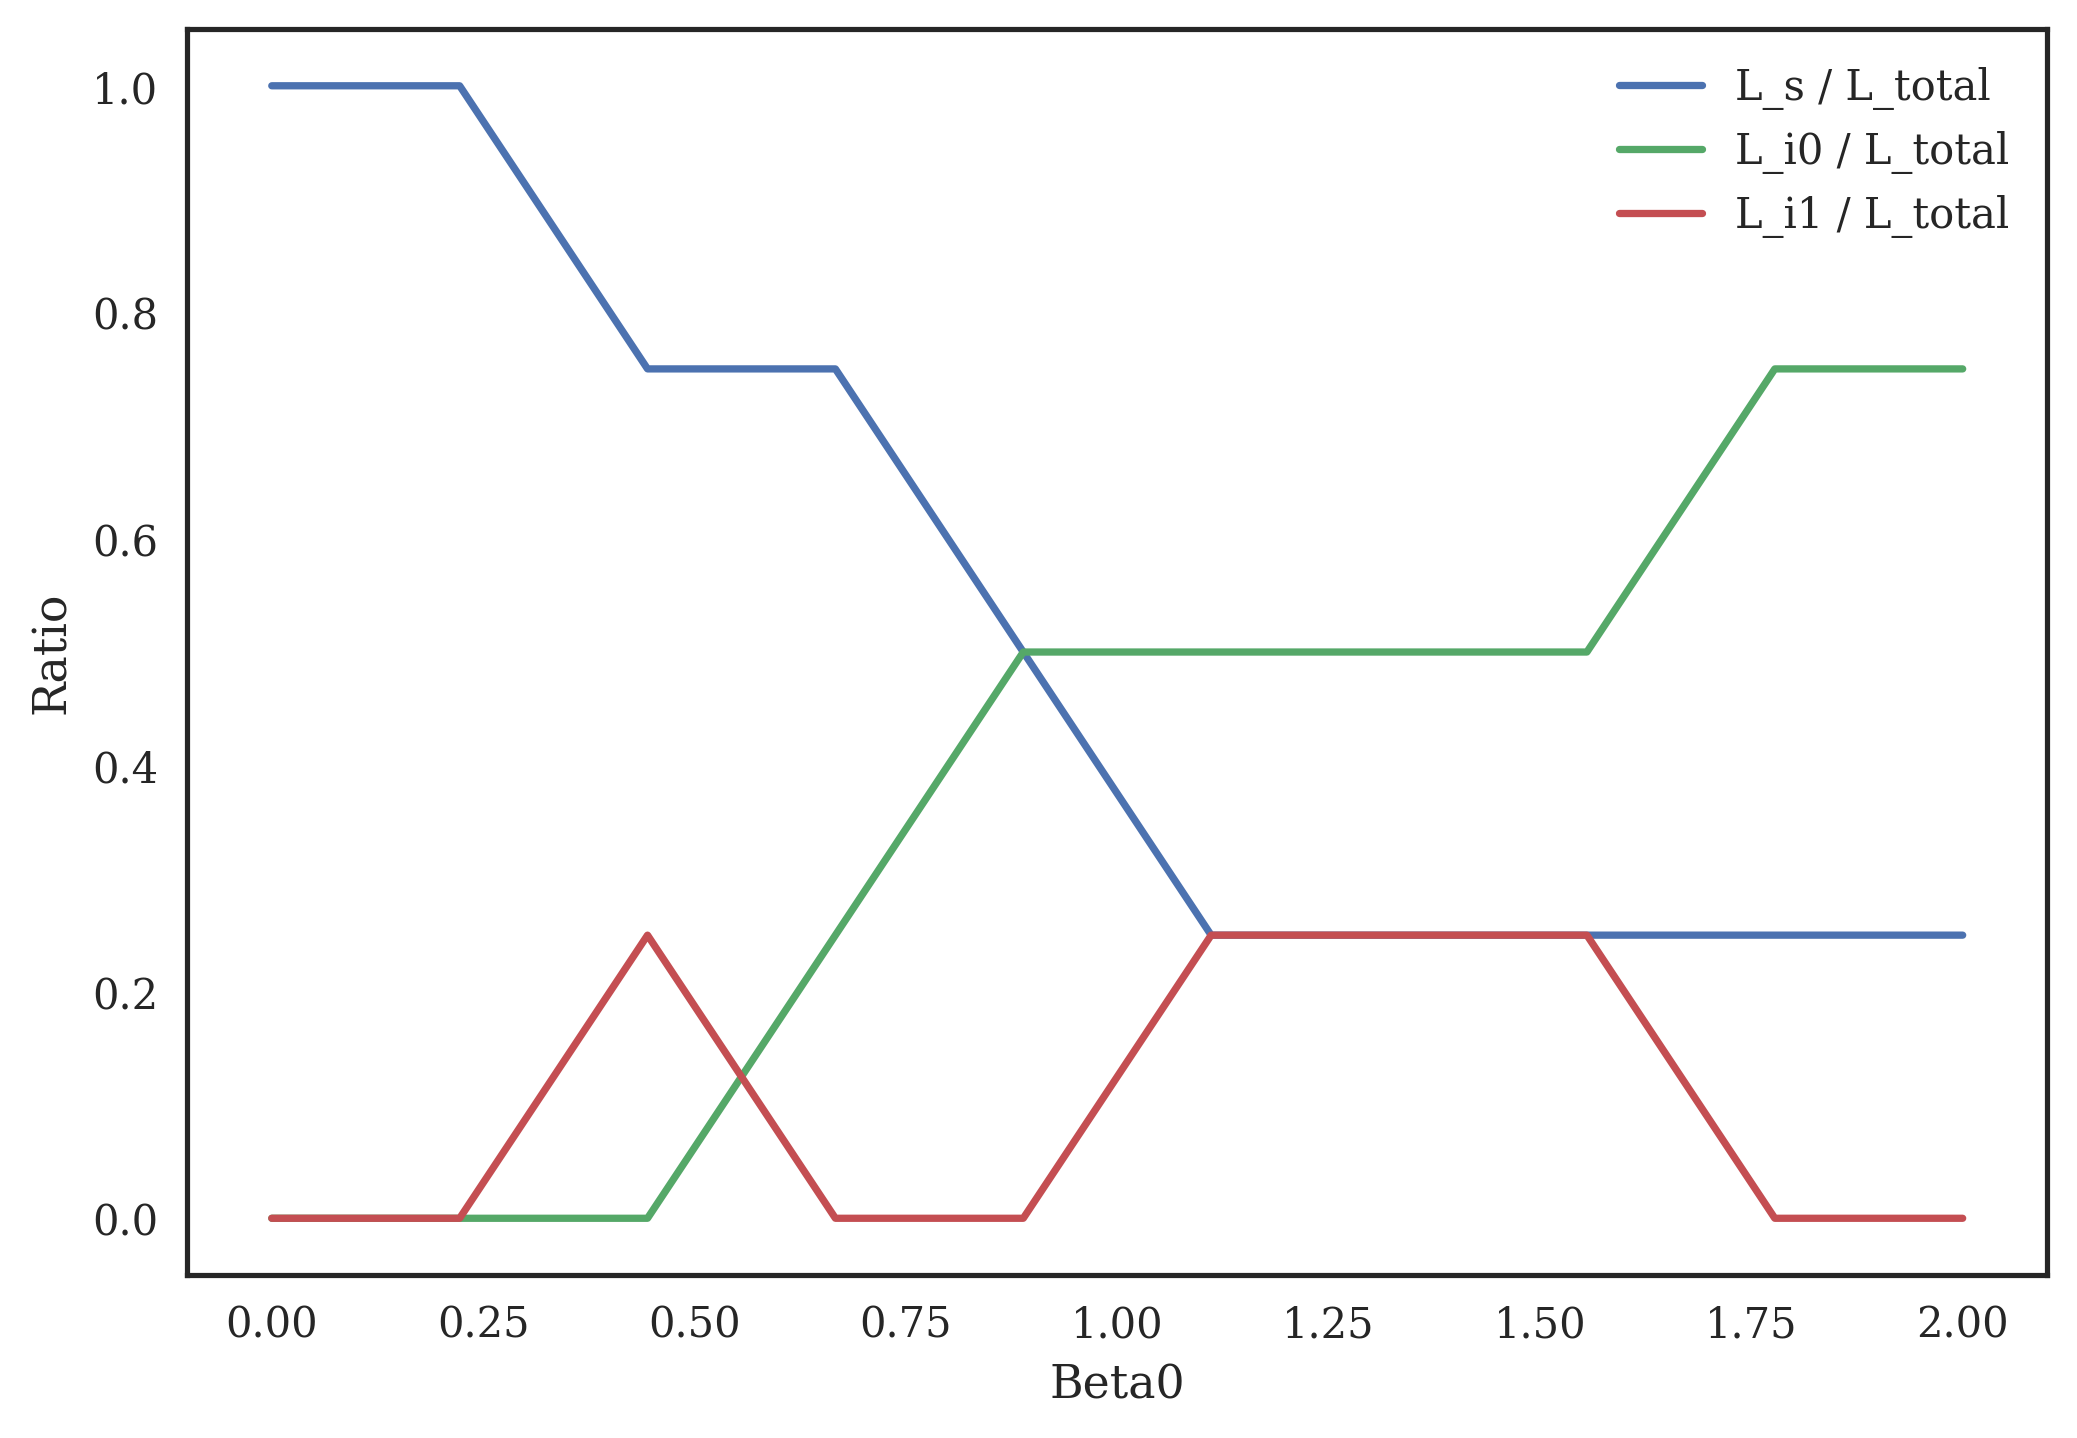
\includegraphics[width=\textwidth]{figures/chapter-5/syn-ratio-beta0.png}
		\caption[Network2]%
		{{Learnt architecture of DCN-LA depending on $\mathbf{C}_0$}}    
		\label{fig:mean and std of net14}
	\end{subfigure}
	\hfill
	\begin{subfigure}[b]{0.475\textwidth}  
		\centering 
		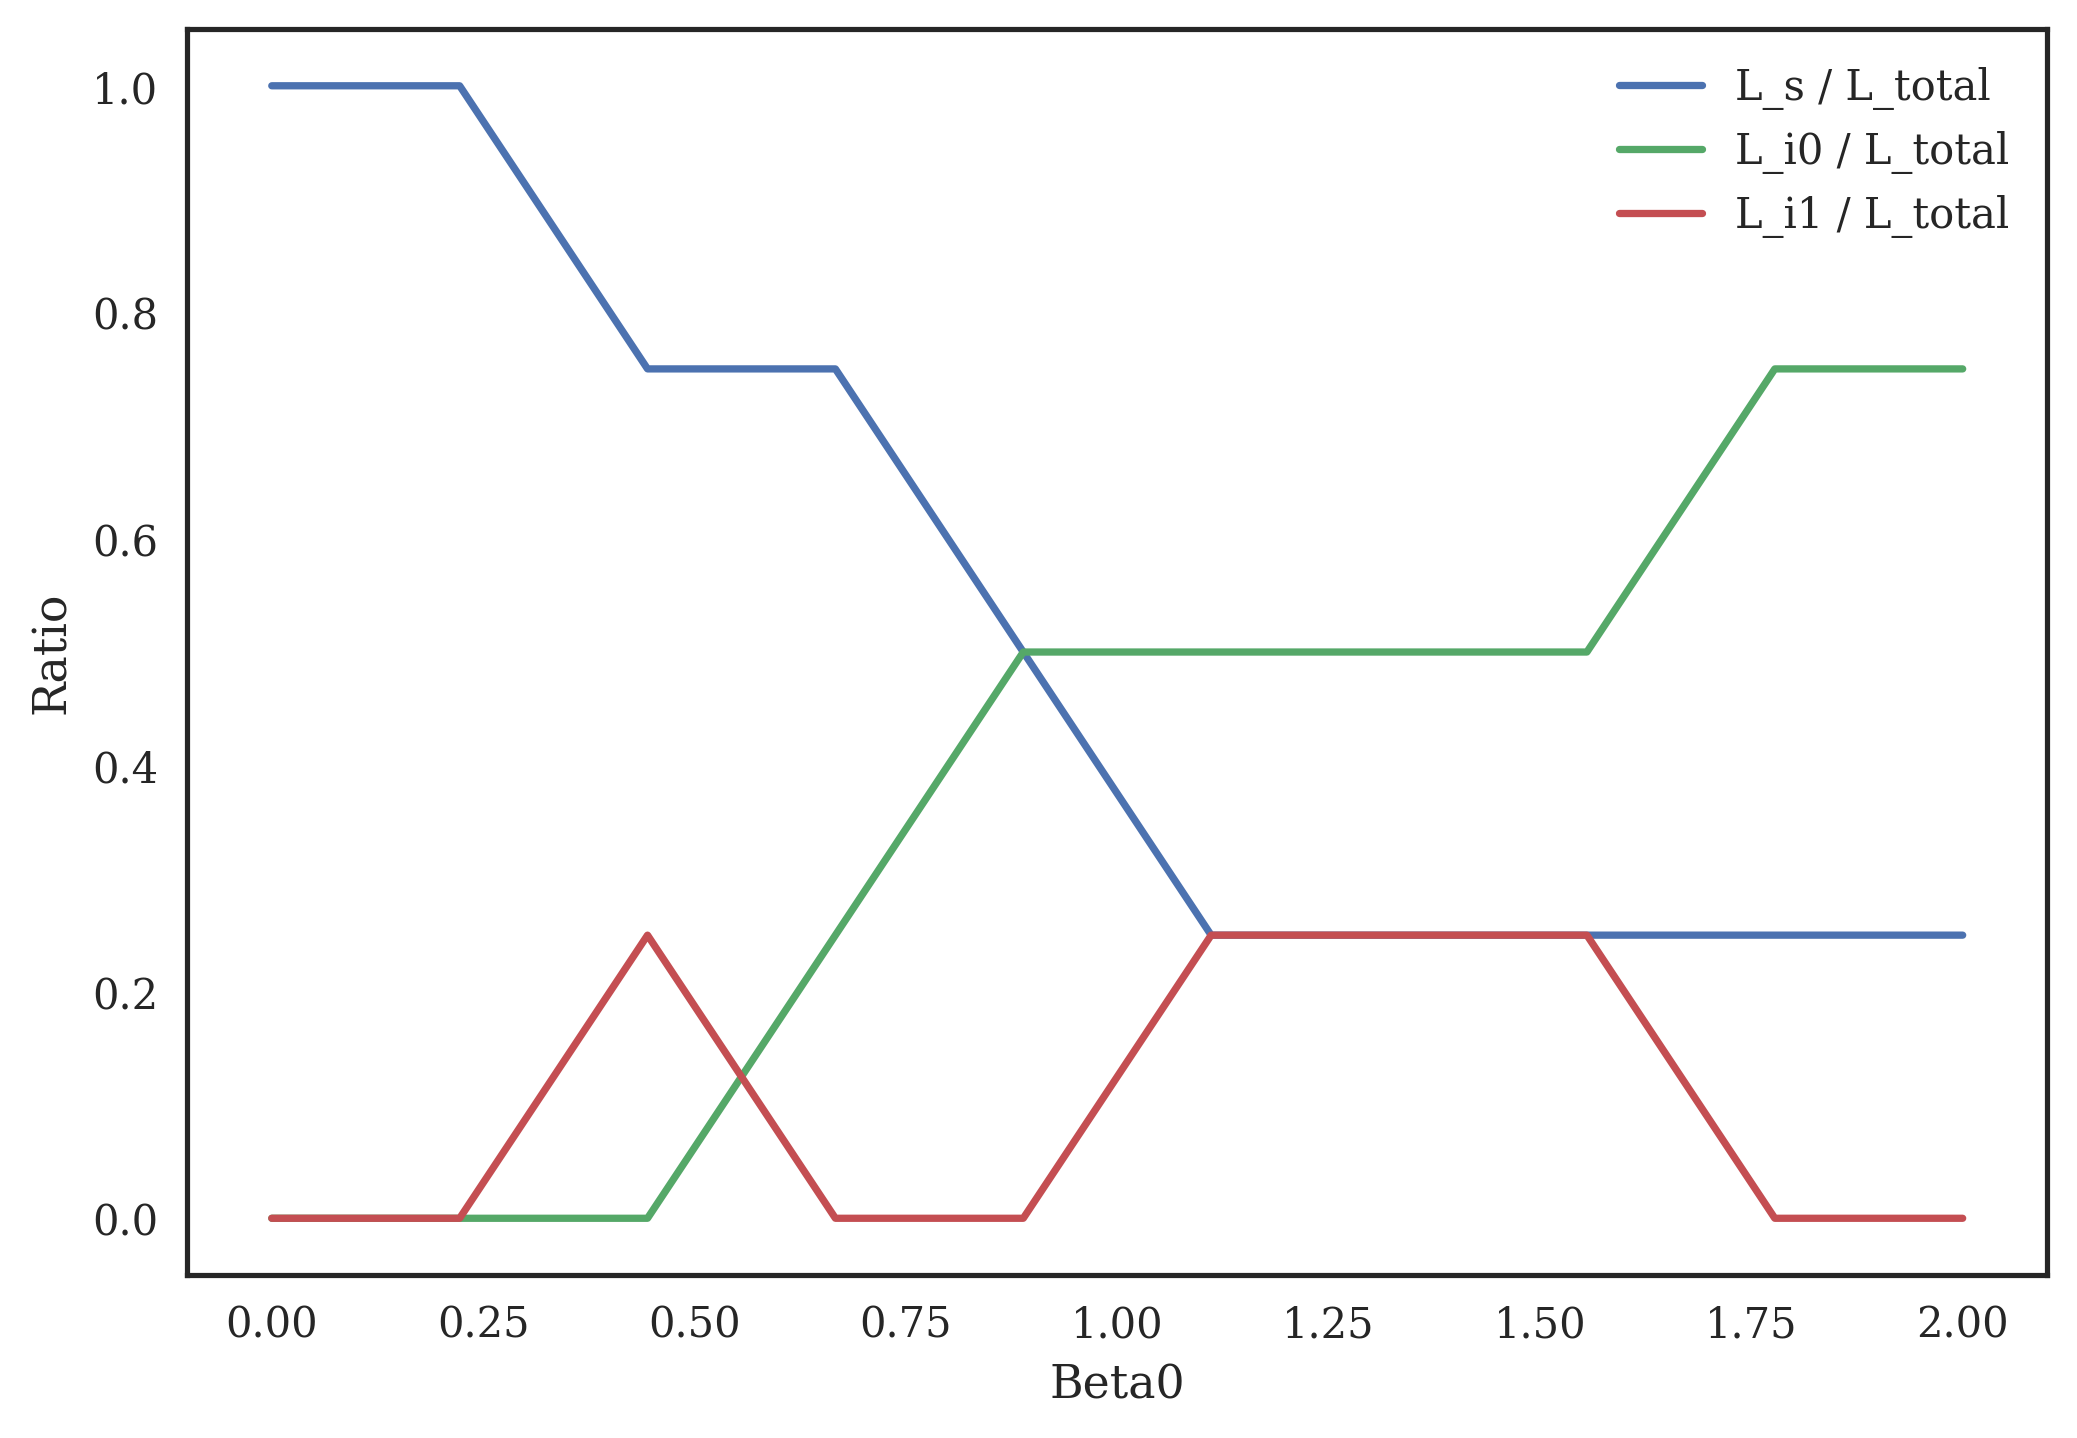
\includegraphics[width=\textwidth]{figures/chapter-5/syn-ratio-beta0.png}
		\caption[]%
		{Learnt architecture of DCN-LA depending on $\mathbf{C}_1$}    
		\label{fig:mean and std of net24}
	\end{subfigure}
	\vskip\baselineskip
	\begin{subfigure}[b]{0.475\textwidth}   
		\centering 
		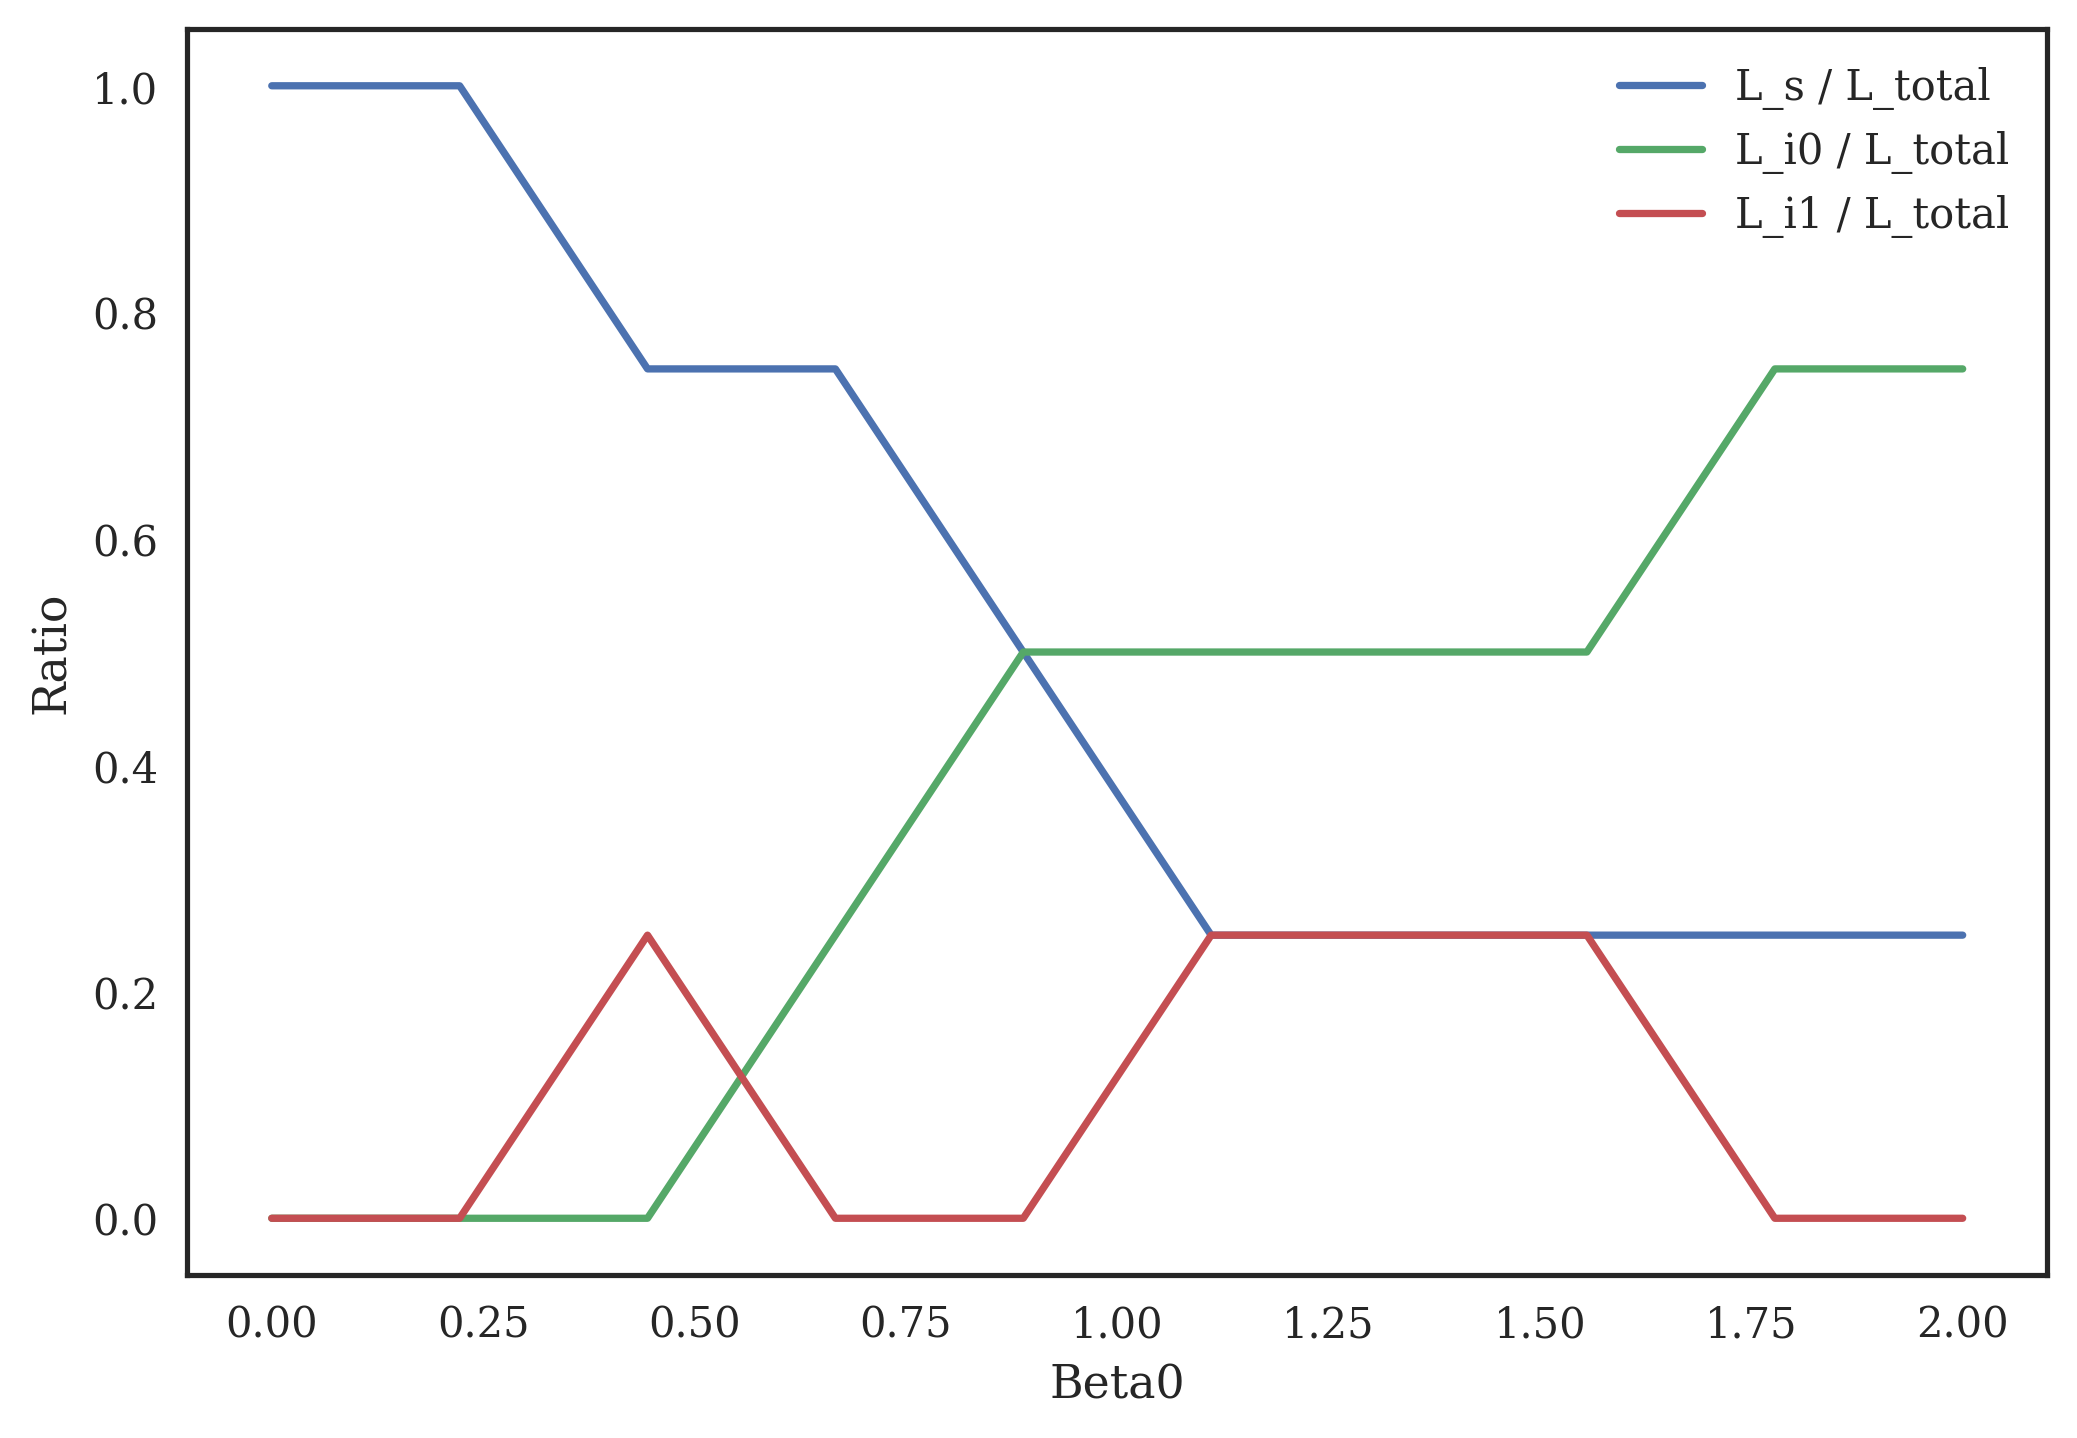
\includegraphics[width=\textwidth]{figures/chapter-5/syn-ratio-beta0.png}
		\caption[]%
		{Performance of DCN-LA depending on $\mathbf{C}_0$}    
		\label{fig:mean and std of net34}
	\end{subfigure}
	\quad
	\begin{subfigure}[b]{0.475\textwidth}   
		\centering 
		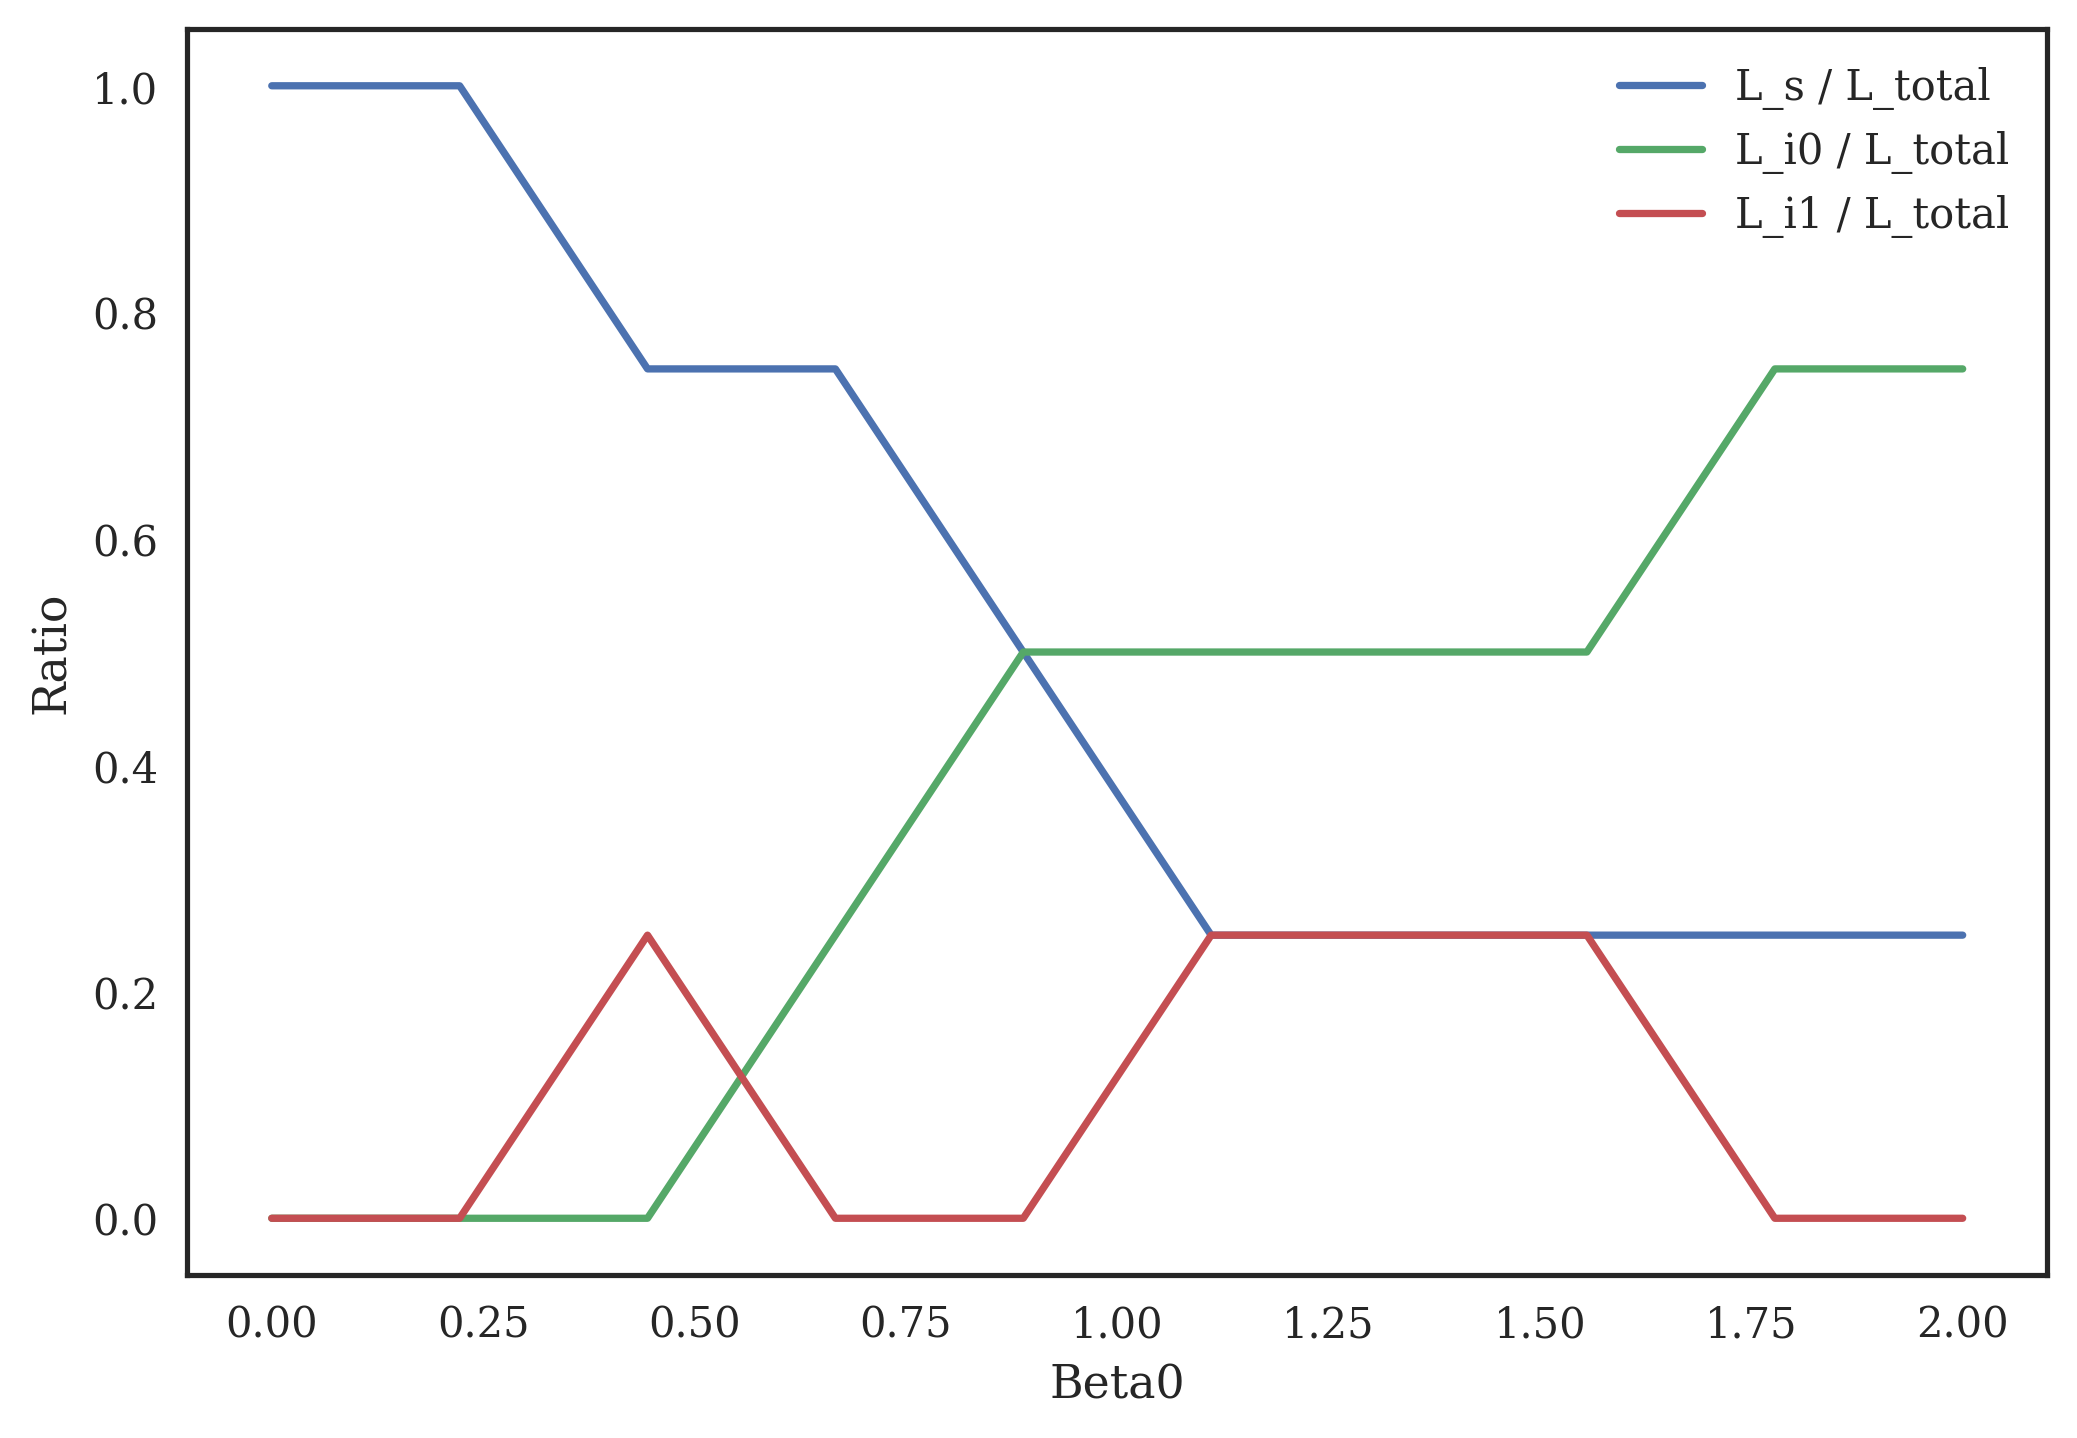
\includegraphics[width=\textwidth]{figures/chapter-5/syn-ratio-beta0.png}
		\caption[]%
		{Performance of DCN-LA depending on $\mathbf{C}_1$}    
		\label{fig:mean and std of net44}
	\end{subfigure}
	
\end{figure}

This observation corresponds well with our intuition that a more complex outcome requires a higher variance of the model reflected in a higher number of layers for the respective outcome. 


The differences between the learnt architectures for $\mathbf{C}_0$ and $\mathbf{C}_1$ can be explained in terms of the selection bias $\mathbf{B}$. The datasets used for the models on the right-hand side were generated with a selection bias of $\mathbf{B} = 0.75$ leading to a higher proportion of the subjects being treated than for the dataset shown on the left-hand side ($\mathbf{B} = 0.5$). As a consequence, the datasets with an strong selection bias are more imbalanced and have a higher number of subjects for the respective outcome, allowing the model to utilise a higher variance for the outcome with the larger population. 


\subsubsection{UNOS}
As we can see in table \ref{tab:dcn-la-results}, the DCN-PD achieves the lowest MSE and outperforms the other methods. The BNN, representing  a strong benchmark as it effectively handles the selection bias by learning a balanced representation for the input features, represents the most competitive alternative. Lastly, the performance gains that our DCN-PD achieves over a the NN-4 model suggest that the multi-task learning framework is an effective conception of counterfactual inference that outperforms direct modelling approaches which consider the treatment assignment as a regular input feature.


\begin{table}[h]
	\centering
	\begin{tabular}{@{}cc@{}}
		\toprule
		\textbf{Algorithm} & \textbf{MSE}                \\ \midrule
		k-NN               &   $5.30 \pm 0.30$           \\
		NN-4                &  $2.88 \pm 0.10$           \\
		DCN                &   $2.58 \pm 0.06$           \\
		DCN-LA             &   $2.05 \pm 0.03$          \\\bottomrule
	\end{tabular}
	\caption{Performance of Deep Counterfactual Networks (DCN) and Deep Counterfactual Networks with Propensity-Dropout (DCN-DP) in comparison with baseline methods and existing competing approaches}\label{tab:dcn-la-results}
\end{table}

\subsection{Discussion}
The results above suggest that our proposed approach of automatically inferring an appropriate DCN architecture based on learnt characteristics of the dataset has the potential to significantly improve the performance of the model by reducing the MSE of the individualised treatment effect. 

As we have seen in the synthetic model, the DCN-LA performs particularly well when dealing with highly-imbalanced data (e.g. high propensity score, little shared complexity, and significantly different outcome surfaces). In these cases the DCN-LA is able to adapt an asymmetric architecture that significantly outperforms symmetric DCNs and other methods. 

However, the results on the UNOS dataset imply that our approach faces difficulties when dealing with real-world data that only expresses subtle imbalances that could be exploited. In these cases, a potential limitation may lie in the fact that the empirical model we use to infer appropriate ratios was pre-trained on \emph{synthetic} datasets that might display different properties and feature distributions than our real-world dataset. 

Nevertheless, even though the performance gain of the DCN-LA on the real-world dataset is marginal, the learnt architecture was derived without the need for computationally expensive hyper-parameter optimisation. So while our model might not always improve the solution quality, it has the potential to drastically reduce the computational costs of the training. 

Concluding, it can be said that our proposed approach of inferring architectures for DCNs by exploiting learnt characteristics of the dataset represents a promising approach that is able to compete with and -- depending on the properties of the dataset -- potentially outperform existing methods. 


\part{Conclusion and Future Work}
%\begin{savequote}[8cm]
%\textlatin{Jedem Anfang wohnt ein Zauber innne.}
%
%In the core of every beginning lives magic.
%  \qauthor{--- Hermann Hesse's \textit{Stufen}}
%\end{savequote}

\chapter{\label{ch:6-conclusion}Conclusion} 

\section{Summary and Contributions}
In the scope of this thesis we have investigated the task of counterfactual inference using deep neural networks. 

In particular, we have introduced the concept of \emph{deep counterfactual networks} (DCNs) that represent a novel approach to causal inference by conceptualising it as a multi-task learning problem. Furthermore, we have proposed \emph{propensity-dropout} (PD), a novel variation of conventional dropout that utilises the individual propensity scores during regularisation. This approach allows us to effectively counteract the problem of classical problem of \emph{covariate shift} between the factual and counterfactual feature distribution caused by the selection bias of the treatment assignment policy. 

Experiments conducted on the \emph{IHDP dataset} in a semi-synthetic setting (typically required for the evaluation of any counterfactual inference task) show that our model of \emph{deep counterfactual networks} with \emph{propensity-dropout} (DCN-PD) outperform the existing methods and provide a significant improvements for the task of counterfactual inference and the prediction of individualised treatment effects. 


In addition, we have introduced an efficient way of automatically learning an appropriate architecture for DCNs by exploiting relevant characteristics of the specific dataset. This is achieved by training an empirical model a-priori on a large number of synthetic datasets for which we can fully control the relevant characteristics.

Concluding, it can be said that our proposed models -- in particular the DCN-PDs -- show promising first results and have the potential of competing and even outperforming the state-of-the-art.

Due to the wide-spread applicability of counterfactual inference, the implications of such an  improvement in this task are highly relevant to a variety of domains such as healthcare, education, economics, and politics -- helping decision-makers in these fields towards more informed and ultimately better interventions. 
%\section{Contributions} %TODO How does it relate to contributions in intro? 

\section{Limitations}
Despite the successes implied by the results of the experiments, it is important to point out limitations and potential shortcomings of our model which might be considered the foundation for future work (see next chapter) in the field of counterfactual inference. 

Firstly, like most existing methods for causal inference our models focus on a \emph{binary} setting in which we are only interested in the outcome or effect of a single treatment which is either present or not. However, the complex governing mechanics that can be found in many real-world problems might require a more general setting in which we are interested in \emph{multiple treatments} and their potential correlations simultaneously.

Secondly, we are currently treating the input features of the context or subject as static, not taking into account any \emph{temporal} dependencies. In many problem areas such as healthcare, however, data typically consists of time-series data (e.g. blood pressure values measured at multiple times during a period of time) which our model is currently not able to accommodate in a way that preserves the temporal information. 

Thirdly, our proposed approach of automatically inferred an appropriate DCN architecture for a given dataset is currently based on an empirical model that was trained on a fully-synthetic dataset. This might be considered a limiting factor for the model to generalise to real-world in cases where the dataset expresses significantly different properties than our empirical model.  

Nevertheless, considering the progress that has been made in the relatively short time frame of the project we are positive that these challenges can be addressed and ultimately overcome in future research.


%
%## DCN-PD:
%- Only works for binary case with a single treatment
%- does not support time series


%\minitoc

%\begin{savequote}[8cm]
%\textlatin{Jedem Anfang wohnt ein Zauber innne.}
%
%In the core of every beginning lives magic.
%  \qauthor{--- Hermann Hesse's \textit{Stufen}}
%\end{savequote}

\chapter{\label{ch:7-future-work}Future Work} 
In the previous chapter we have discussed the findings of the project, the contributions of our models, and their potential limitations. Consequently, we provide a list of open research questions that can be considered the subject of future work in the field of counterfactual inference. 

\paragraph{Multiple Treatments} In order to address more complex real-world problems, it would be of great interest to investigate how our models can be generalised towards a multi-variate setting in which we are dealing with multiple feature assignments simultaneously. The multi-task learning framework that we are using for DCNs should in theory be able to accommodate non-binary setting with more than two separate but related tasks. However, additional challenges such as the interdependence and joint effects of the treatments have to be taken into account as well posing a variety of open research questions. 

\paragraph{Time-Series Data} It would be of great relevance to investigate how our models can be extended to time-series input data that contains temporal dependencies between the features. Future work in this field might examine the effectiveness of a multi-task framework with propensity-dropout to a recurrent neural network. 

\paragraph{Extensions of Propensity-Dropout} While our proposed propensity-based dropout scheme provides promising first results in the experiments, it would be interesting to investigate how the propensity score could also be used in competing regularising approaches such as DropConnect. % CITE Dropconnect

\paragraph{Empirical Model for Architecture Learning} Our approach of automatically inferring an appropriated DCN architecture is based on an empirical model that is trained in a supervised setting on synthetically-generated datasets. Due to the very nature of such a heuristic approach, the empirical model should be subject to ongoing research and improvements. In particular, it could be beneficial to analyse how we can ensure that the synthetically-generated have similar properties to real-world datasets in order to allow a maximum level of generalisation.  


%## DCN-PD:
%- Multiple treatments?
%- Time series data? 
%- Can we adapt our multi-class learning to an RNN? 
%- Propensity-based DropConnect?
%
%## DCN-LA:
%- Run data on other datasets
%- Improve empirical model (more training data, other heuristics to infer the charactistics, etc.)
%- More experiments, 
%- Other features? 


%\minitoc


%\begin{savequote}[8cm]
Alles Gescheite ist schon gedacht worden.\\
Man muss nur versuchen, es noch einmal zu denken.

All intelligent thoughts have already been thought;\\
what is necessary is only to try to think them again.
  \qauthor{--- Johann Wolfgang von Goethe \cite{von_goethe_wilhelm_1829}}
\end{savequote}

\chapter{\label{ch:2-litreview}Background}

\minitoc

\section{Introduction}

This document introduction won't serve as a complete primer on \LaTeX.  There are plenty of those online, and googling your questions will often get you answers, especially from \url{http://tex.stackexchange.com}.

Instead, let's talk a little about a few of the features and packages lumped into this template situation.  The \verb|savequote| environment at the beginning of chapters can add some wittiness to your thesis.  If you don't like the quotes, just remove that block.

For when it comes time to do corrections, there are two useful commands here.  First, the \verb|mccorrect| command allows you to highlight a short correction \mccorrect{like this one}.  When the thesis is typeset normally, the correction will just appear as part of the text.  However, when you declare \verb|\correctionstrue| in the main \verb|Oxford_Thesis.tex| file, that correction will be highlighted in blue.  That might be useful for submitting a post-viva, corrected copy to your examiners so they can quickly verify you've completed the task.

\begin{mccorrection}
For larger chunks, like this paragraph or indeed entire figures, you can use the \verb|mccorrection| environment.  This environment highlights paragraph-sized and larger blocks with the same blue colour.
\end{mccorrection}

Read through the \verb|Oxford_Thesis.tex| file to see the various options for one- and two-sided printing, including or excluding the separate abstract page, and turning corrections and draft footer on or off, and the separate option to centre your text on the page (for PDF submission) or offset it (for binding).  There is also a separate option for master's degree submissions, which changes identifying information to candidate number and includes a word count.  (Unfortunately, \LaTeX has a hard time doing word counts automatically, so you'll have to enter the count manually if you require this.)

\section{Cardiac Imaging}\label{app:imaging}

Within months of Röntgen's discovery of the X-ray in \mccorrect{1895}\cite{gagliardi_rontgen_1996}, cardiac pathology was being investigated via non-invasive imaging \cite{gagliardi_cardiac_1996}.  Over the intervening years, cardiac imaging modalities and techniques have advanced significantly.  Clinically, cardiac imaging is used for two broad purposes: diagnosis of pathophysiology and guidance of interventional procedures.  These applications impose different requirements on imaging equipment, image acquisition time, computational complexity, spatial and temporal resolution, and tissue discrimination.  The common diagnostic and interventional cardiac imaging techniques in current clinical practice are reviewed below.  An accessible introduction to the physics of medical imaging can be found in Webb's \textit{Introduction to Biomedical Imaging} \cite{webb_introduction_2002}.  A comprehensive overview of the use of imaging in clinical cardiology is presented in Leeson's \textit{Cardiovascular Imaging} \cite{leeson_cardiovascular_2011}.

\subsection{Diagnostic Imaging}
\label{sub:diagnostic}

Beyond the chest X-ray (`plain film'), the key non-invasive imaging modalities in diagnostic cardiology are echocardiography, magnetic resonance imaging, and X-ray computed tomography, which are reviewed below.  Nuclear medicine, including positron emission tomography (PET) and single-photon emission computed tomography (SPECT), are not discussed here, as they do not play a role in the chapters to follow.

\subsubsection{Echocardiography}

\begin{figure}
\centering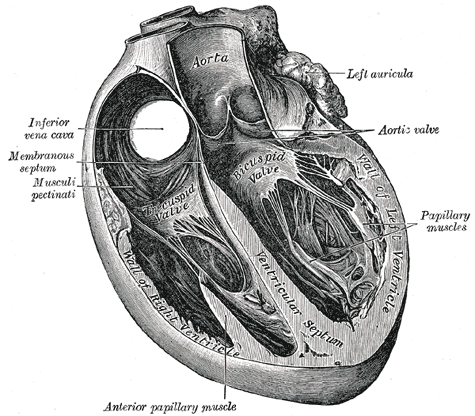
\includegraphics[width=0.7\textwidth]{figures/sample/Gray498.png} 
\caption[Four-chamber illustration of the human heart.]{Four-chamber illustration of the human heart.  Clockwise from upper-left: right atrium, left atrium, left ventricle, right ventricle.}
\label{fig:fourchamber}\end{figure}

The use of acoustic waves for medical diagnosis, inspired by naval sonar, was initially developed in the 1940s \cite{gagliardi_ultrasonography_1996}.  By 1954, the first clinically useful cardiac ultrasound -- examining motion of the mitral valve in stenosis -- was reported \cite{edler_ultrasonic_1957}.  These early scans were one-dimensional images (`A-mode'), sometimes repeated to generate a time axis (`M-mode').   The sector-scanning probe was developed in the 1970s \cite{bom_ultrasonic_1971,griffith_sector_1974}, leading to the `B-mode' that a modern cardiologist would recognise as an echocardiogram.



%% APPENDICES %% 
% Starts lettered appendices, adds a heading in table of contents, and adds a
%    page that just says "Appendices" to signal the end of your main text.
% META Check if I need an appendix
%\startappendices
% Add or remove any appendices you'd like here:
%\begin{savequote}[8cm]
\textlatin{Cor animalium, fundamentum e\longs t vitæ, princeps omnium, Microco\longs mi Sol, a quo omnis vegetatio dependet, vigor omnis \& robur emanat.}

The heart of animals is the foundation of their life, the sovereign of everything within them, the sun of their microcosm, that upon which all growth depends, from which all power proceeds.
  \qauthor{--- William Harvey \cite{harvey_exercitatio_1628}}
\end{savequote}

\chapter{\label{app:1-cardiophys}Review of Cardiac Physiology and Electrophysiology}

\minitoc

Appendices are just like chapters.  Their sections and subsections get numbered and included in the table of contents; figures and equations and tables added up, etc.  Lorem ipsum dolor sit amet, consectetur adipiscing elit. Sed et dui sem. Aliquam dictum et ante ut semper. Donec sollicitudin sed quam at aliquet. Sed maximus diam elementum justo auctor, eget volutpat elit eleifend. Curabitur hendrerit ligula in erat feugiat, at rutrum risus suscipit. Pellentesque habitant morbi tristique senectus et netus et malesuada fames ac turpis egestas. Integer risus nulla, facilisis eget lacinia a, pretium mattis metus. Vestibulum aliquam varius ligula nec consectetur. Maecenas ac ipsum odio. Cras ac elit consequat, eleifend ipsum sodales, euismod nunc. Nam vitae tempor enim, sit amet eleifend nisi. Etiam at erat vel neque consequat.

\section{Anatomy}
\label{sec:anatomy}

Lorem ipsum dolor sit amet, consectetur adipiscing elit. Donec accumsan cursus neque. Pellentesque eget tempor turpis, quis malesuada dui. Proin egestas, sapien sit amet feugiat vulputate, nunc nibh mollis nunc, nec auctor turpis purus sed metus. Aenean consequat leo congue volutpat euismod. Vestibulum et vulputate nisl, at ultrices ligula. Cras pulvinar lacinia ipsum at bibendum. In ac augue ut ante mollis molestie in a arcu.

Etiam vitae quam sollicitudin, luctus tortor eu, efficitur nunc. Vestibulum maximus, ante quis consequat sagittis, augue velit luctus odio, in scelerisque arcu magna id diam. Proin et mauris congue magna auctor pretium id sit amet felis. Maecenas sit amet lorem ipsum. Proin a risus diam. Integer tempus eget est condimentum faucibus. Suspendisse sem metus, consequat vel ante eget, porttitor maximus dui. Nunc dapibus tincidunt enim, non aliquam diam vehicula sed. Proin vel felis ut quam porta tempor. Vestibulum elit mi, dictum eget augue non, volutpat imperdiet eros. Praesent ac egestas neque, et vehicula felis.

Pellentesque malesuada volutpat justo, id eleifend leo pharetra at. Pellentesque feugiat rutrum lobortis. Curabitur hendrerit erat porta massa tincidunt rutrum. Donec tincidunt facilisis luctus. Aliquam dapibus sodales consectetur. Suspendisse lacinia, ipsum sit amet elementum fermentum, nulla urna mattis erat, eu porta metus ipsum vel purus. Fusce eget sem nisl. Pellentesque dapibus, urna vitae tristique aliquam, purus leo gravida nunc, id faucibus ipsum magna aliquet ligula. Lorem ipsum dolor sit amet, consectetur adipiscing elit. Proin sem lacus, rutrum eget efficitur sed, aliquam vel augue. Aliquam ut eros vitae sem cursus ultrices ut ornare urna. Nullam tempor porta enim, in pellentesque arcu commodo quis. Interdum et malesuada fames ac ante ipsum primis in faucibus. Curabitur maximus orci purus, ut molestie turpis pellentesque ut.

Donec lacinia tristique ultricies. Proin dignissim risus ut dolor pulvinar mollis. Proin ac turpis vitae nibh finibus ullamcorper viverra quis felis. Mauris pellentesque neque diam, id feugiat diam vestibulum vitae. In suscipit dui eu libero ultrices, et sagittis nunc blandit. Aliquam at aliquet ex. Nullam molestie pulvinar ex vitae interdum. Praesent purus nunc, gravida id est consectetur, convallis elementum nulla. Praesent ex dolor, maximus eu facilisis at, viverra eget nulla. Donec ullamcorper ante nisi. Sed volutpat diam eros. Nullam egestas neque non tortor aliquet, sed pretium velit tincidunt. Aenean condimentum, est ac vestibulum mattis, quam augue congue augue, mattis ultrices nibh libero non ante. Lorem ipsum dolor sit amet, consectetur adipiscing elit.

Aenean volutpat eros tortor, non convallis sapien blandit et. Maecenas faucibus nulla a magna posuere commodo. Nullam laoreet ante a turpis laoreet malesuada. Phasellus in varius sem. Vestibulum sagittis nibh sed tincidunt blandit. Donec aliquam accumsan odio sit amet lacinia. Integer in tellus diam. Vivamus varius massa leo, vitae ullamcorper metus pulvinar sed. Maecenas nec lorem ornare, elementum est quis, gravida massa. Suspendisse volutpat odio ex, ac ultrices leo ultrices vel. Sed sed convallis ipsum. Pellentesque euismod a nulla sed rhoncus. Sed vehicula urna vitae mi aliquet, non sodales lacus ullamcorper. Duis mattis justo turpis, id tempus est tempus eu. Curabitur vitae hendrerit ligula.

Curabitur non pretium enim, in commodo ligula. Etiam commodo eget ligula a lacinia. Vestibulum laoreet ante tellus, vel congue sapien ornare in. Donec venenatis cursus velit vitae pulvinar. Pellentesque habitant morbi tristique senectus et netus et malesuada fames ac turpis egestas. Suspendisse in metus lectus. Pellentesque gravida dolor eget finibus imperdiet. Duis id molestie tortor. Mauris laoreet faucibus facilisis. Aliquam vitae dictum massa, sit amet dignissim lacus.

Fusce eleifend tellus id ex consequat maximus. Donec ultrices ex ut turpis ornare, non molestie mi placerat. Nulla sit amet auctor nunc, sit amet euismod elit. Phasellus risus tellus, condimentum a metus et, venenatis tristique urna. Cras mattis felis eget ipsum fermentum egestas. Ut augue odio, venenatis id convallis vel, congue quis augue. Maecenas sed maximus est, posuere aliquet tortor. Ut condimentum egestas nisi eu porttitor. Ut mi turpis, posuere id lorem vel, elementum tempor arcu.

Morbi nisl arcu, venenatis non metus ac, ullamcorper scelerisque justo. Nulla et accumsan lorem. Mauris aliquet dui sit amet libero aliquet, in ornare metus porttitor. Integer ultricies urna eu consequat ultrices. Maecenas a justo id purus ultricies posuere sed et quam. Cum sociis natoque penatibus et magnis dis parturient montes, nascetur ridiculus mus. Sed eleifend risus quis aliquet gravida. Nullam ac erat porta est bibendum dictum in a dolor. Nam eget turpis viverra, vulputate lectus eget, mattis ligula. Nam at tellus eget dui lobortis sodales et ut augue. In vestibulum diam eget mi cursus, ut tincidunt nulla pellentesque.

Aliquam erat volutpat. Sed ultrices massa id ex mattis bibendum. Nunc augue magna, ornare at aliquet gravida, vehicula sed lorem. Quisque lobortis ipsum eu posuere eleifend. Duis bibendum cursus viverra. Nam venenatis elit leo, vitae feugiat quam aliquet sed. Cras velit est, tempus ac lorem sed, pharetra lobortis ipsum. Donec suscipit gravida interdum. Nunc non finibus est. Nullam turpis elit, tempus non ante.

\section{Mechanical Cycle}

Lorem ipsum dolor sit amet, consectetur adipiscing elit. Aenean tellus est, suscipit sed facilisis quis, malesuada at ipsum. Nam tristique urna quis quam iaculis, et mattis orci pretium. Praesent euismod elit vel metus commodo ultrices. Vestibulum et tincidunt ex, in molestie ex. Donec ullamcorper sollicitudin accumsan. Etiam ac leo turpis. Duis a tortor felis. Nullam sollicitudin eu purus ac hendrerit. Nam hendrerit ligula libero, eget finibus orci bibendum a. Aenean ut ipsum magna.

Ut viverra, sapien sed accumsan blandit, nisi sem tempus tellus, at suscipit magna erat ornare nunc. Proin lacinia, nisi ut rutrum malesuada, nibh quam pellentesque nunc, sit amet consectetur purus felis ac tortor. Suspendisse lacinia ipsum eu sapien pellentesque mattis. Mauris ipsum nunc, placerat non diam vel, efficitur laoreet nunc. Sed lobortis, ipsum eget gravida facilisis, sem nulla viverra mi, in placerat eros sem viverra lacus. Aliquam porta aliquet diam vel commodo. Nulla facilisi. Duis erat libero, lobortis vel hendrerit vitae, sagittis id dui. Nulla pretium eros nec quam tincidunt, vel luctus mi aliquam. Integer imperdiet purus in est tristique venenatis. Ut pellentesque, nunc vitae iaculis ultricies, urna turpis dignissim risus, a laoreet felis magna nec erat.

Quisque sollicitudin faucibus ligula, et egestas nibh dictum sit amet. Proin eu mi a lectus congue pretium eu quis arcu. Suspendisse vehicula libero eu ipsum aliquam, vel elementum nibh mattis. Sed sed sapien vitae turpis tristique pulvinar a ut metus. Etiam semper gravida est, mollis gravida est porta ac. Proin eget tincidunt erat. Maecenas ultrices erat eget purus ultricies, ut lacinia arcu dictum. Nam et nisi sit amet ex congue mattis vel eget lorem. Aliquam erat volutpat. Pellentesque porttitor nibh vitae elementum consectetur. Aenean et est lobortis, congue sapien non, ullamcorper sapien. Ut facilisis sem non dapibus vehicula.

Mauris euismod odio dolor, sit amet gravida mauris placerat et. Curabitur nec dolor non nibh molestie lobortis dignissim non ante. Nullam rutrum lobortis ultrices. Aenean ex erat, elementum sed maximus id, posuere id quam. Proin rutrum ex elit, pretium aliquam risus finibus at. Aenean egestas orci velit, sed aliquet sapien condimentum a. Duis consequat, arcu eu viverra venenatis, dolor lorem gravida lectus, non aliquet nisi sem at augue. Donec laoreet blandit luctus. Aenean vehicula nisl vel faucibus luctus. Sed ut semper velit, vitae laoreet magna. Sed at interdum magna.

Sed iaculis faucibus odio, eu aliquam purus efficitur vel. Cras at nulla ac enim congue varius ut et nulla. Integer blandit mattis augue.

\section{Electrical Cycle}
\label{sec:electcycle}

Lorem ipsum dolor sit amet, consectetur adipiscing elit. In faucibus condimentum rhoncus. Ut dictum nisl id risus gravida lobortis. Sed vehicula mollis tellus ut varius. Fusce eget egestas dui, et commodo dui. Proin sollicitudin interdum tempus. Nullam in elit a enim fringilla bibendum. Vestibulum sodales pellentesque condimentum. Nulla facilisi. Nunc et dolor in nulla eleifend dictum at vel ligula. Aliquam ut velit non elit ullamcorper porta ac et ex. Fusce ornare magna non nunc vestibulum, eget molestie quam dictum. In interdum aliquam odio, in posuere tellus convallis quis. Curabitur non diam elit. Proin vulputate orci diam, a tincidunt ante luctus eu. Ut a viverra ligula. Curabitur pulvinar tempus tellus eget suscipit.

Aliquam posuere massa at ante dapibus congue. Curabitur ullamcorper tortor eget consectetur aliquet. Mauris tempor magna id mauris fringilla, a varius erat blandit. Nam eleifend ullamcorper placerat. Phasellus augue tortor, volutpat bibendum lorem nec, fringilla volutpat nisl. Mauris cursus urna metus, vel eleifend orci iaculis ut. Sed sit amet scelerisque massa, quis consequat dui. Donec semper sem dui, ac placerat velit egestas vel. Nulla facilisi. Quisque tellus eros, sagittis malesuada augue ut, faucibus dictum nulla. Vestibulum non dapibus erat, ut consequat libero. Ut turpis mi, dapibus commodo libero lobortis, maximus vestibulum lectus. Vestibulum sit amet sapien dapibus, tincidunt leo in, suscipit arcu. Sed in erat bibendum, laoreet eros eu, pellentesque justo. Nulla sodales purus neque, eget maximus ipsum consequat at. Maecenas a nisl sagittis, tempus ipsum sed, dictum mauris.

Suspendisse posuere odio lacus, at auctor tortor vehicula sed. Phasellus suscipit ornare enim vitae placerat. Sed viverra purus vel sapien tempor, quis iaculis erat laoreet. Aenean vel nunc vestibulum, ornare nunc ac, mollis urna. Aenean ultrices felis ipsum, ac semper est ullamcorper in. Donec in justo varius, egestas tortor ut, venenatis augue. Duis mattis, ligula quis lacinia fringilla, tellus neque accumsan ipsum, vitae tempor metus elit vel nibh. Curabitur porttitor urna nec sapien tempor, et porttitor velit malesuada.

Suspendisse aliquam nisl quis placerat vulputate. Proin dapibus ipsum ac ante sagittis, volutpat auctor sem dapibus. Nam in facilisis odio. Integer ante mauris, eleifend et pulvinar in, venenatis quis ligula. Phasellus posuere sollicitudin tortor eget euismod. Maecenas mollis tortor eget justo vulputate sagittis. Etiam hendrerit massa quis ex molestie sodales. Quisque facilisis erat lacus, id convallis sem suscipit bibendum. Integer dui urna, pharetra sed porta sed, bibendum ut odio. Donec placerat at lectus egestas consequat. Sed id rhoncus est, vitae vulputate sapien. Fusce tempus quam lorem, id ornare turpis sodales sed. Integer aliquet urna eget condimentum consequat. Vestibulum quis dui vel ligula posuere luctus id nec turpis.

Nam vitae placerat lacus. Mauris scelerisque interdum volutpat. Nunc aliquet tristique enim, sit amet molestie felis ullamcorper vitae. Nullam sollicitudin orci orci, in condimentum tellus consectetur in. Nam id justo justo. Fusce eget finibus est. Proin id tortor nec quam cursus vehicula. Aliquam ultrices eros eros, a tincidunt elit eleifend auctor.

Nullam consectetur dapibus ligula sit amet efficitur. Nunc non posuere sapien. Vivamus dui nisl, aliquam id ipsum non, pulvinar ornare neque. Nunc rhoncus pretium congue. Fusce id laoreet enim. Cras sed massa in eros bibendum auctor in nec sem. Nam commodo, velit id porta consequat, mi arcu gravida lorem, ut aliquam elit ante quis dui. Quisque in massa sed nibh blandit dictum.

Vestibulum molestie consectetur porttitor. Donec tincidunt vel orci at pharetra. Nullam id felis sit amet nulla tempus lacinia. Integer egestas ullamcorper massa, ut ultricies diam congue sit amet. Cras sit amet velit at nibh vehicula finibus a et lorem. Cras odio metus, venenatis ut ultrices non, ornare ac orci. Morbi et nulla dui. Mauris dictum molestie nibh, eu efficitur lorem accumsan quis.

\section{Cellular Electromechanical Coupling}
\label{sec:electromech}

Lorem ipsum dolor sit amet, consectetur adipiscing elit. Nullam vitae consectetur metus, ac maximus ex. Quisque vitae ex eu lectus ultricies consequat vel non lorem. Etiam odio ipsum, tempus ut lobortis in, molestie ac leo. Vivamus mollis feugiat bibendum. Vestibulum eget venenatis quam. Aenean faucibus, massa sed ullamcorper porta, arcu nunc iaculis velit, quis consectetur purus neque placerat nibh. Vestibulum elit nunc, dignissim vulputate venenatis et, sodales non massa. Proin leo ligula, vehicula eu aliquam varius, posuere a dolor. Donec iaculis auctor neque, sit amet gravida libero porta vel. Vivamus consequat elementum lacus, at bibendum mauris egestas nec. Fusce fermentum diam eu dolor ornare, vitae vestibulum leo interdum. Morbi luctus libero quis dictum laoreet. Etiam semper porta ante, vel ullamcorper enim sodales quis.

Nullam eu nisi faucibus, fermentum ex auctor, tempor arcu. Phasellus condimentum erat mi, condimentum malesuada ligula congue venenatis. Nullam gravida imperdiet urna quis cursus. Ut tempus nec purus eget posuere. Cras non nulla sit amet justo aliquet pellentesque nec sed eros. Nam aliquam nisl urna, in placerat magna gravida venenatis. Donec interdum vel magna ullamcorper molestie. Nunc felis neque, rhoncus fringilla faucibus sit amet, ultrices sed magna. Maecenas malesuada hendrerit diam in ultrices. Nam libero urna, volutpat ut auctor eget, interdum sed odio. Vestibulum suscipit mauris nec augue ornare, ut eleifend nulla gravida. Proin imperdiet, mauris quis consectetur porta, leo dui convallis leo, id lobortis massa diam eu libero. Aenean hendrerit vel ante aliquam venenatis. Pellentesque bibendum pretium odio, ut sagittis lectus feugiat a. Donec porttitor vulputate lacus.

Nunc volutpat efficitur lacus in aliquet. Nullam non iaculis diam, at ultrices diam. Proin vehicula vulputate cursus. Morbi tempus sapien id urna lobortis interdum. Maecenas elementum sagittis elementum. Donec at sodales velit, a posuere tortor. Nulla id hendrerit tortor. Sed semper velit in magna sagittis pulvinar. Nulla nec arcu molestie, ultricies sapien sit amet, sollicitudin nisi. Donec nisi massa, suscipit ut dignissim quis, lacinia id leo.

Suspendisse ut mi metus. Morbi tincidunt ligula in porttitor consectetur. Integer eu urna urna. Suspendisse potenti. Mauris sit amet felis eu diam auctor ullamcorper. Morbi in porta nisi. Nam ante tortor, venenatis vitae tempor sed, sagittis vitae velit. In semper orci sit amet nisi ullamcorper varius. Aenean dignissim ultrices imperdiet. Maecenas lacinia enim id neque porttitor iaculis. Curabitur laoreet ante ut urna dignissim, id sollicitudin metus consectetur. Aenean massa ipsum, auctor vel ante vel, blandit dignissim libero. Fusce interdum ac magna et interdum.


% FINAL Remove this:
\nocite{dummy-source}

%%%%% REFERENCES

% Quote for the top of references (just like a chapter quote if you're using them).  Comment to skip.
%\begin{savequote}[8cm]
%The first kind of intellectual and artistic personality belongs to the hedgehogs, the second to the foxes \dots
%  \qauthor{--- Sir Isaiah Berlin \cite{berlin_hedgehog_2013}}
%\end{savequote}

\setlength{\baselineskip}{0pt} % Single-space References

{\renewcommand*\MakeUppercase[1]{#1}%
\printbibliography[heading=bibintoc,title={\bibtitle}]}


\end{document}
